%% 
%DIF LATEXDIFF DIFFERENCE FILE


%% Copyright 2019-2020 Elsevier Ltd
%% 
%% This file is part of the 'CAS Bundle'.
%% --------------------------------------
%% 
%% It may be distributed under the conditions of the LaTeX Project Public
%% License, either version 1.2 of this license or (at your option) any
%% later version.  The latest version of this license is in
%%    http://www.latex-project.org/lppl.txt
%% and version 1.2 or later is part of all distributions of LaTeX
%% version 1999/12/01 or later.
%% 
%% The list of all files belonging to the 'CAS Bundle' is
%% given in the file `manifest.txt'.
%% 
%% Template article for cas-dc documentclass for 
%% double column output.

%\documentclass[a4paper,fleqn,longmktitle]{cas-dc}
% \documentclass[a4paper,fleqn]{cas-dc}
\documentclass{singlecol-new}

%\usepackage[authoryear,longnamesfirst]{natbib}
%\usepackage[authoryear]{natbib}
\usepackage[numbers]{natbib}

\usepackage{amsmath,amssymb}
\usepackage{longtable}
%%%
\usepackage{mathtools}
\allowdisplaybreaks
\usepackage{algorithm,algorithmic}
\DeclarePairedDelimiter{\ceil}{\lceil}{\rceil}		
\DeclarePairedDelimiter{\floor}{\lfloor}{\rfloor}
\usepackage{url}
%DIF PREAMBLE EXTENSION ADDED BY LATEXDIFF
%DIF UNDERLINE PREAMBLE %DIF PREAMBLE
\RequirePackage[normalem]{ulem} %DIF PREAMBLE
\RequirePackage{color}\definecolor{RED}{rgb}{1,0,0}\definecolor{BLUE}{rgb}{0,0,1} %DIF PREAMBLE
\providecommand{\DIFadd}[1]{{\protect\color{blue}\uwave{#1}}} %DIF PREAMBLE
\providecommand{\DIFdel}[1]{{\protect\color{red}\sout{#1}}}                      %DIF PREAMBLE
%DIF SAFE PREAMBLE %DIF PREAMBLE
\providecommand{\DIFaddbegin}{} %DIF PREAMBLE
\providecommand{\DIFaddend}{} %DIF PREAMBLE
\providecommand{\DIFdelbegin}{} %DIF PREAMBLE
\providecommand{\DIFdelend}{} %DIF PREAMBLE
\providecommand{\DIFmodbegin}{} %DIF PREAMBLE
\providecommand{\DIFmodend}{} %DIF PREAMBLE
%DIF FLOATSAFE PREAMBLE %DIF PREAMBLE
\providecommand{\DIFaddFL}[1]{\DIFadd{#1}} %DIF PREAMBLE
\providecommand{\DIFdelFL}[1]{\DIFdel{#1}} %DIF PREAMBLE
\providecommand{\DIFaddbeginFL}{} %DIF PREAMBLE
\providecommand{\DIFaddendFL}{} %DIF PREAMBLE
\providecommand{\DIFdelbeginFL}{} %DIF PREAMBLE
\providecommand{\DIFdelendFL}{} %DIF PREAMBLE
%DIF END PREAMBLE EXTENSION ADDED BY LATEXDIFF

\begin{document}
%\let\WriteBookmarks\relax

\JOURNALNAME{\TEN{\it Int. J. of Data Mining and Bioinformatics, Vol. \theVOL, No. \theISSUE, \thePUBYEAR}\hfill\thepage}%


\VOL{x}

\ISSUE{x}

\PUBYEAR{202X}

\BottomCatch

\CLline


\def\floatpagepagefraction{1}
\def\textpagefraction{.001}


\title{GRASP-based Heuristic with Data Mining for the Prize Collecting Covering Tour problem}                      
%\tnotemark[1,2]

%\tnotetext[1]{This document is the results of the research
%   project funded by the National Science Foundation.}
%
%\tnotetext[2]{The second title footnote which is a longer text matter
%   to fill through the whole text width and overflow into
%   another line in the footnotes area of the first page.}





%\credit{Conceptualization of this study, Methodology, Software}



%\author[2,4]{Han Theh Thanh}[style=chinese]

%\author[2,3]{CV Rajagopal}[%
%   role=Co-ordinator,
%   suffix=Jr,
%   ]
%\fnmark[2]
%\ead{cvr3@sayahna.org}
%\ead[URL]{www.sayahna.org}

%\credit{Data curation, Writing - Original draft preparation}

%\address[2]{Sayahna Foundation, Jagathy, Trivandrum 695014, India}

%\author%
%[1,3]
%{Rishi T.}
%\cormark[2]
%\fnmark[1,3]
%\ead{rishi@stmdocs.in}
%\ead[URL]{www.stmdocs.in}

%\address[3]{STM Document Engineering Pvt Ltd., Mepukada,
%    Malayinkil, Trivandrum 695571, India}

%\cortext[cor2]{Principal corresponding author}
%\fntext[fn1]{This is the first author footnote. but is common to third
%  author as well.}
%\fntext[fn2]{Another author footnote, this is a very long footnote and
%  it should be a really long footnote. But this footnote is not yet
%  sufficiently long enough to make two lines of footnote text.}

%\nonumnote{This note has no numbers. In this work we demonstrate $a_b$
%  the formation Y\_1 of a new type of polariton on the interface
%  between a cuprous oxide slab and a polystyrene micro-sphere placed
%  on the slab.
%  }

\begin{abstract}

\DIFdelbegin \DIFdel{The investigation of hybrid heuristicsis very present in recent researches related to combinatorial optimisation. Hybridisation with Greedy Randomized }\DIFdelend \DIFaddbegin \DIFadd{Recent research has shown that hybrid heuristics, combining Greedy Randomised }\DIFaddend Adaptive Search Procedures (GRASP) \DIFdelbegin \DIFdel{and data miningis a successful example in the literature, where }\DIFdelend \DIFaddbegin \DIFadd{with data mining, are an effective approach to solving combinatorial optimisation problems. This paper presents a novel hybrid heuristic for the prize-collecting covering tour problem, which employs data mining techniques to enhance the GRASP algorithm. By leveraging }\DIFaddend patterns observed in \DIFdelbegin \DIFdel{a }\DIFdelend high-quality \DIFdelbegin \DIFdel{solution can lead to effective exploration of }\DIFdelend \DIFaddbegin \DIFadd{solutions, our approach is able to explore }\DIFaddend the search space \DIFdelbegin \DIFdel{and a large decrease in }\DIFdelend \DIFaddbegin \DIFadd{more efficiently, leading to improved results and reduced }\DIFaddend computational time. \DIFdelbegin \DIFdel{In this work, data mining techniques are used to enhance a GRASP state-of-the-art heuristic for the prize-collecting covering tour problem.
Computational results revealed that the data mining proposals were able to match or enhance solution quality for a wide number of instances while also reducing execution time significantly. Statistical }\DIFdelend \DIFaddbegin \DIFadd{Our experimental results demonstrate the effectiveness of the proposed approach, which consistently outperforms existing methods across a wide range of problem instances. We present statistical }\DIFaddend significance tests, \DIFdelbegin \DIFdel{evaluations of the influence of mining patterns, }\DIFdelend \DIFaddbegin \DIFadd{as well as an analysis of the impact of pattern mining }\DIFaddend and time-to-target plots\DIFdelbegin \DIFdel{are presented to back up }\DIFdelend \DIFaddbegin \DIFadd{, to support }\DIFaddend our findings.

\end{abstract}



\DIFdelbegin %DIFDELCMD < \KEYWORD{Data mining; hybrid heuristic; GRASP;  prize-collecting covering tour problem.}
%DIFDELCMD < %%%
\DIFdelend \DIFaddbegin \KEYWORD{Data mining; Hybrid heuristics; Greedy Randomised Adaptive Search Procedures (GRASP);  Prize-collecting covering tour problem.}
\DIFaddend 


\maketitle

\section{Introduction}
\label{sec:intro}

\DIFdelbegin \DIFdel{Metaheuristics are commonly employed to tackle combinatorial optimisation problems , providing approximate solutions in }\DIFdelend \DIFaddbegin \DIFadd{Combinatorial optimization problems can be challenging to solve exactly, but metaheuristics offer a way to obtain good approximate solutions within }\DIFaddend a reasonable amount of time. \DIFdelbegin \DIFdel{Greedy Randomized }\DIFdelend \DIFaddbegin \DIFadd{One well-known metaheuristic is Greedy Randomised }\DIFaddend Adaptive Search Procedures (GRASP)\DIFdelbegin \DIFdel{is a well-known metaheuristic that has been effectively }\DIFdelend \DIFaddbegin \DIFadd{, which has been successfully }\DIFaddend applied to a \DIFdelbegin \DIFdel{variety of combinatorial optimisation }\DIFdelend \DIFaddbegin \DIFadd{wide range of combinatorial optimization }\DIFaddend problems \cite{resende2019greedy}.

\DIFdelbegin \DIFdel{The investigation of hybrid heuristicshas been shown to be very present in recent researches related to combinatorial optimisation. Such heuristics often }\DIFdelend \DIFaddbegin \DIFadd{Recent research on combinatorial optimization has increasingly focused on hybrid heuristics, which }\DIFaddend combine different heuristics \DIFdelbegin \DIFdel{, even from different aspects and paradigms \mbox{%DIFAUXCMD
\cite{talbi2009metaheuristics}}\hskip0pt%DIFAUXCMD
.
Hybrid metaheuristics can also include principles from other fieldsof study}\DIFdelend \DIFaddbegin \DIFadd{from multiple paradigms and domains \mbox{%DIFAUXCMD
\cite{talbi2009metaheuristics}}\hskip0pt%DIFAUXCMD
. These hybrid metaheuristics can draw upon principles from diverse fields}\DIFaddend , such as data mining (DM), to \DIFdelbegin \DIFdel{increase its }\DIFdelend \DIFaddbegin \DIFadd{improve their }\DIFaddend efficiency and adaptability. \DIFdelbegin \DIFdel{According to \mbox{%DIFAUXCMD
\citet{han2011data}}\hskip0pt%DIFAUXCMD
, DM can be referred as the automatic extraction of knowledge from data-sets}\DIFdelend \DIFaddbegin \DIFadd{DM involves automatically extracting knowledge from data sets}\DIFaddend , which can \DIFaddbegin \DIFadd{then }\DIFaddend be represented by rules or patterns \DIFaddbegin \DIFadd{\mbox{%DIFAUXCMD
\cite{han2011data}}\hskip0pt%DIFAUXCMD
}\DIFaddend .

\DIFdelbegin \DIFdel{The objective behind using DMmethods }\DIFdelend \DIFaddbegin \DIFadd{One motivation for applying data mining (DM) techniques }\DIFaddend in heuristics is to extract patterns from \DIFdelbegin \DIFdel{good quality solutions }\DIFdelend \DIFaddbegin \DIFadd{high-quality solutions and use those patterns }\DIFaddend to guide the search \DIFdelbegin \DIFdel{procedures. For the set packing problem, for example, \mbox{%DIFAUXCMD
\citet{ribeiro06} }\hskip0pt%DIFAUXCMD
developed the }\DIFdelend \DIFaddbegin \DIFadd{process. For instance, \mbox{%DIFAUXCMD
\citet{ribeiro06} }\hskip0pt%DIFAUXCMD
proposed }\DIFaddend DM-GRASP, a hybrid heuristic \DIFdelbegin \DIFdel{combining the GRASP metaheuristic }\DIFdelend \DIFaddbegin \DIFadd{that combines GRASP }\DIFaddend with DM techniques \DIFdelbegin \DIFdel{. The main idea of }\DIFdelend \DIFaddbegin \DIFadd{to solve the set packing problem. }\DIFaddend DM-GRASP \DIFdelbegin \DIFdel{is to extract }\DIFdelend \DIFaddbegin \DIFadd{extracts }\DIFaddend patterns from high-quality solutions \DIFdelbegin \DIFdel{and then utilise those patterns }\DIFdelend to build initial solutions in a later phase. This \DIFdelbegin \DIFdel{data mining approach was also used to a number of problemsas a consequence of its promising outcomes}\DIFdelend \DIFaddbegin \DIFadd{approach has been applied to various optimization problems}\DIFaddend , such as the \DIFdelbegin \DIFdel{2-path network design problem \mbox{%DIFAUXCMD
\cite{barbalho2013}}\hskip0pt%DIFAUXCMD
, the }\DIFdelend p-median problem \cite{plastino2011hybrid}, the \DIFdelbegin \DIFdel{point‐feature }\DIFdelend \DIFaddbegin \DIFadd{point-feature }\DIFaddend cartographic label placement problem \cite{guerine2020hybrid}, and the server replication for reliable multi-cast problem \cite{santos2006ngl01}\DIFaddbegin \DIFadd{, with promising results}\DIFaddend .

\DIFdelbegin \DIFdel{Moreover}\DIFdelend \DIFaddbegin \DIFadd{To improve upon DM-GRASP}\DIFaddend , \citet{plastino2011hybrid} introduced \DIFdelbegin \DIFdel{a }\DIFdelend \DIFaddbegin \DIFadd{an adaptive variant, called }\DIFaddend multi DM-GRASP (MDM-GRASP), \DIFdelbegin \DIFdel{an adaptive variant of the DM-GRASP }\DIFdelend for the p-median problem. Unlike \DIFdelbegin \DIFdel{the }\DIFdelend DM-GRASP\DIFdelbegin \DIFdel{technique, which only conducts }\DIFdelend \DIFaddbegin \DIFadd{, which performs }\DIFaddend the DM process \DIFdelbegin \DIFdel{once, the }\DIFdelend \DIFaddbegin \DIFadd{only once, }\DIFaddend MDM-GRASP \DIFdelbegin \DIFdel{approach performs }\DIFdelend \DIFaddbegin \DIFadd{conducts }\DIFaddend the DM process \DIFdelbegin \DIFdel{anytime }\DIFdelend \DIFaddbegin \DIFadd{again when }\DIFaddend the elite set \DIFdelbegin \DIFdel{becomes stable. Herein, this stability }\DIFdelend \DIFaddbegin \DIFadd{stabilizes. The elite set }\DIFaddend refers to a \DIFdelbegin \DIFdel{number of iterations in which the elite set does not change. In practice, }\DIFdelend \DIFaddbegin \DIFadd{subset of }\DIFaddend the \DIFaddbegin \DIFadd{best solutions found by the heuristic. The MDM-GRASP approach gradually improves the }\DIFaddend general quality of the elite set\DIFdelbegin \DIFdel{is gradually improved throughout the execution, giving }\DIFdelend \DIFaddbegin \DIFadd{, leading to }\DIFaddend more refined patterns\DIFdelbegin \DIFdel{each time. In fact, the MDM version outperformed the original heuristic }\DIFdelend \DIFaddbegin \DIFadd{. In practice, MDM-GRASP outperformed DM-GRASP }\DIFaddend and was slightly better than the \DIFdelbegin \DIFdel{DM version's }\DIFdelend \DIFaddbegin \DIFadd{original heuristic }\DIFaddend in terms of solution quality and computational time \cite{plastino2014adaptive}.

In this work, we \DIFdelbegin \DIFdel{present }\DIFdelend \DIFaddbegin \DIFadd{propose }\DIFaddend a hybrid DM method based on MDM-GRASP \DIFdelbegin \DIFdel{for tackling }\DIFdelend \DIFaddbegin \DIFadd{to solve }\DIFaddend the prize-collecting covering tour problem (PCCTP)\DIFdelbegin \DIFdel{. PCCTP, a covering tour problem(CTP) \mbox{%DIFAUXCMD
\cite{gendreau1997covering} }\hskip0pt%DIFAUXCMD
variation, is a route planning problem in which the goal is to construct a minimum length tour on a subset of vertices (with prizes associated) such that every vertex to be covered is within a pre-specified distance from the cycle, and a minimum prize is collected }\DIFdelend \DIFaddbegin \DIFadd{, a well-known combinatorial optimization problem. The objective of PCCTP is to find a minimum-cost tour that covers a set of nodes with certain prizes and collects the prizes along the tour. The goal is to minimize the tour cost, subject to the constraint that the sum of the collected prizes is at least a given threshold }\DIFaddend \cite{gendreau1997covering}.

%DIF <  For the DM strategy proposal, we have hybridized a state-of-the-art heuristic denoted as GRASP-GENIUS-RVND, which was introduced by \cite{daSilva} for the PCCTP. Also, it is important to emphasize that  the authors generously provided the original source code of GILS-RVND as well as all seeds of pseudo-random numbers used in the Silva et al. (2012) experiments, allowing us to completely re-run the original experiments of this heuristic, allowing for a fair comparison between the heuristics evaluated in this paper. 
\DIFdelbegin %DIFDELCMD < 

%DIFDELCMD < %%%
%DIF <  The following is a formal definition of the PCCTP. Consider the undirected graph G = (N,E), which has the vertices N = V?W and V = R?T, as well as the edges E = (vi, vj)|vi, vj? V, I j. Let D denote the coverage distance, and ce denote the cost associated with it.
%DIFDELCMD < 

%DIFDELCMD < %%%
%DIF <  Each e? E and pi should be paired with a prize for each vertex I V. Let T be a subset that includes
%DIFDELCMD < 

%DIFDELCMD < %%%
%DIF <  the vertices that must be visited, and R a subset of optional vertices, and as a result
%DIFDELCMD < 

%DIFDELCMD < %%%
%DIF <  It is possible that you will be visited. Finally, consider W as a subset containing the required vertices.
%DIFDELCMD < 

%DIFDELCMD < %%%
%DIF <  If cij? D is true, then a vertex I V covers a vertex j?W.
%DIFDELCMD < 

%DIFDELCMD < %%%
\DIFdel{The following is a formal definition for the PCCTP. Let $G = (N,E)$ be }\DIFdelend \DIFaddbegin \DIFadd{The Prize Collecting Covering Tour Problem (PCCTP) is an important optimisation problem in the field of combinatorial optimisation. It involves finding a minimum cost cycle that covers a set of vertices with certain prizes while also collecting the prizes along the cycle. Formally, the PCCTP can be defined as follows: Given }\DIFaddend an undirected graph \DIFdelbegin \DIFdel{, which has the vertices $N = V \cup W $ and $V = R \cup T$,  as well as the set of edges$E = \{(v_i,v_j)|v_i,v_j \in V, i < j \}$. Let $D$ denote the coverage distance, $c_e$ denote the respective cost for each $e \in E $ }\DIFdelend \DIFaddbegin \DIFadd{$G=(N,E)$, where $N=V\cup W$ represents the vertices }\DIFaddend and \DIFdelbegin \DIFdel{$p_i$  be a prize for visiting a vertex  $i \in V$. Consider }\DIFdelend \DIFaddbegin \DIFadd{$E={(v_i,v_j)|v_i,v_j \in V, i < j}$ represents the edges. The vertices are partitioned into two subsets $V=R\cup T$, where }\DIFaddend $T$ \DIFdelbegin \DIFdel{as a subset }\DIFdelend \DIFaddbegin \DIFadd{is the set }\DIFaddend of vertices that \DIFdelbegin \textit{\DIFdel{must}} %DIFAUXCMD
\DIFdelend \DIFaddbegin \DIFadd{must }\DIFaddend be visited and $R$ \DIFdelbegin \DIFdel{as a subset }\DIFdelend \DIFaddbegin \DIFadd{is the set }\DIFaddend of optional vertices that may or may not be visited. \DIFdelbegin \DIFdel{Lastly, consider  }\DIFdelend \DIFaddbegin \DIFadd{The vertices in }\DIFaddend $W$ \DIFdelbegin \DIFdel{to be a subset of the vertices that }\DIFdelend must be covered by another vertex\DIFaddbegin \DIFadd{, defined as $c_{ij}\leq D$, where $D$ is the coverage distance and $c_e$ represents the respective cost for each edge $e\in E$. Finally, $p_i$ represents a prize associated with visiting a vertex $i\in V$. An illustration of the problem is provided in Figure \ref{fig:pcctp}}\DIFaddend .
\DIFdelbegin \DIFdel{For example, if a vertex $i \in V$ covers a vertex $j \in W$ then  $c_{ij} \leq D$. The PCCTP seeks to find a minimum cost cycle which visits all vertices in $T$, while covers all vertices in $W$ and collects  a minimum prize (see Figure \ref{fig:pcctp}). 
}\DIFdelend 

%DIF <  The PCCTP seeks to identify a simple minimum cost cycle that visits all vertices in T, covers all vertices in the subsetW, and collects at least a minimum prize (PRIZE). Figure 1 shows a workable solution for a small instance with the value of PRIZE set to 100.
\DIFdelbegin %DIFDELCMD < 

%DIFDELCMD < %%%
\DIFdelend \begin{figure}[h]
	\centering
	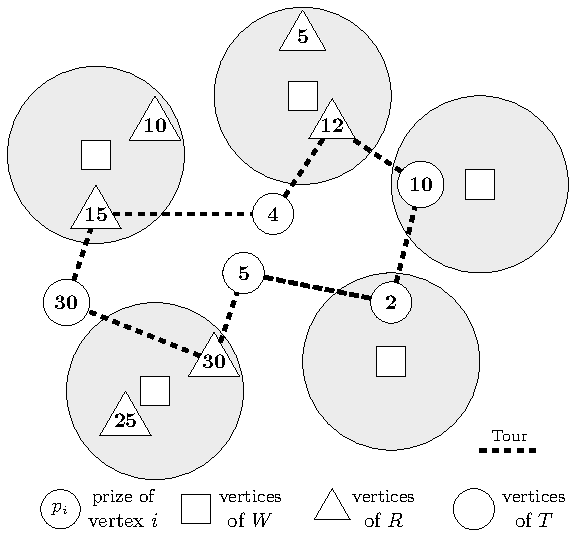
\includegraphics[width=0.45\textwidth]{pcctp-solution.pdf}
	\caption{\DIFdelbeginFL \DIFdelFL{A }\DIFdelendFL \DIFaddbeginFL \DIFaddFL{An example of a }\DIFaddendFL feasible solution for a small instance with the value of $PRIZE$ set to 100.}
	\label{fig:pcctp}
\end{figure}

\DIFdelbegin \DIFdel{According to \mbox{%DIFAUXCMD
\citet{daSilva}}\hskip0pt%DIFAUXCMD
, }\DIFdelend \DIFaddbegin \DIFadd{In their study, \mbox{%DIFAUXCMD
\citet{daSilva} }\hskip0pt%DIFAUXCMD
present }\DIFaddend a real-world scenario for the \DIFdelbegin \DIFdel{PCCTP may be found in the supply of a tour for }\DIFdelend \DIFaddbegin \DIFadd{Prize Collecting Covering Tour Problem (PCCTP). In this scenario, the vertices in set $T$ represent essential cities that need to be visited by }\DIFaddend itinerant vehicles providing social services. The vertices \DIFdelbegin \DIFdel{of $T$ are considered as important cities in an area that are specified as necessary visiting points, whereas the vertices of $R$ }\DIFdelend \DIFaddbegin \DIFadd{in set $R$, on the other hand, }\DIFaddend refer to optional stop locations \DIFdelbegin \DIFdel{. For set }\DIFdelend \DIFaddbegin \DIFadd{for the vehicles. Set }\DIFaddend $W$ \DIFdelbegin \DIFdel{, it would contain }\DIFdelend \DIFaddbegin \DIFadd{includes }\DIFaddend locations that are difficult to \DIFdelbegin \DIFdel{access, and then to serve their respective people, the vehicle would have }\DIFdelend \DIFaddbegin \DIFadd{reach, requiring the vehicles }\DIFaddend to pass through a location \DIFdelbegin \DIFdel{(}\DIFdelend \DIFaddbegin \DIFadd{within a coverage distance of $D$ to serve their residents, whether in }\DIFaddend $T$ or $R$\DIFdelbegin \DIFdel{) of up to $D$ units of distance. For }\DIFdelend \DIFaddbegin \DIFadd{. To ensure that }\DIFaddend the vehicle release \DIFdelbegin \DIFdel{to be worthwhile}\DIFdelend \DIFaddbegin \DIFadd{is economically feasible}\DIFaddend , a minimum \DIFdelbegin \DIFdel{quantity of people must be attended. As a result, }\DIFdelend \DIFaddbegin \DIFadd{number of residents must be served, and }\DIFaddend each vertex's prize represents the population of each city\DIFdelbegin \DIFdel{to be visited, and the total prize to be collected refers to the minimum total number of residents to be serviced}\DIFdelend \DIFaddbegin \DIFadd{. The total prize collected represents the minimum total population of residents that must be served.
}

\DIFadd{Another real-life application of the PCCTP is in public transportation. For instance, a public transit system may have to plan the optimal route for a bus or train that covers a set of stations with varying demand, where each station has a certain prize representing the number of passengers to be picked up or dropped off. However, it may not be possible or cost-effective to stop at all the stations, and some stations may have to be skipped. In such a scenario, the PCCTP can be used to find the optimal route that covers the stations with the highest prizes while minimizing the cost of the route. This problem can also be extended to include additional constraints, such as time limits or the maximum number of passengers that can be carried on the vehicle}\DIFaddend .

The \DIFdelbegin \DIFdel{remainder of the paper is structured }\DIFdelend \DIFaddbegin \DIFadd{paper is organized }\DIFaddend as follows. Section \ref{sec:grasp} \DIFdelbegin \DIFdel{presents a short review }\DIFdelend \DIFaddbegin \DIFadd{provides a brief overview }\DIFaddend of the literature on PCCTP and \DIFdelbegin \DIFdel{provides details of }\DIFdelend \DIFaddbegin \DIFadd{describes }\DIFaddend the state-of-the-art heuristic \DIFaddbegin \DIFadd{in detail}\DIFaddend . Section \ref{sec:datamining} \DIFdelbegin \DIFdel{details }\DIFdelend \DIFaddbegin \DIFadd{explains }\DIFaddend the proposed data mining approaches. \DIFdelbegin \DIFdel{Computational results are shown and analysed in Section \ref{sec:computationalresults}}\DIFdelend \DIFaddbegin \DIFadd{In Section \ref{sec:computationalresults}, we present and analyze the computational results}\DIFaddend . Finally, in Section \ref{sec:conclusions}\DIFdelbegin \DIFdel{the conclusions are drawn and some future works are pointed out}\DIFdelend \DIFaddbegin \DIFadd{, we draw conclusions and highlight future work}\DIFaddend .

\section{\DIFdelbegin \DIFdel{GRASP-GENIUS-RVND: }\DIFdelend The state-of-the-art heuristic}

\label{sec:grasp}

Few authors have discussed the PCCTP before and some solution methods have been presented. \citep{lyra2004problema} introduced the PCCTP and as solution methods, proposed a mathematical formulation \DIFdelbegin \DIFdel{the }\DIFdelend \DIFaddbegin \DIFadd{that }\DIFaddend makes use of flow constraints to eliminate sub-tours, and a GRASP-based heuristic  \citep{grasp03}   associated with a VNS (Variable Neighbourhood Search) metaheuristic \citep{mladenovic97}.  Also, a path-relinking strategy was used as an intensification component for trying to improve solutions.

Next, \citet{silva2009problema} introduced  six new heuristics,  which are based on the ILS (Iterated Local Search) metaheuristic and evolutionary algorithms. Finally, \citet{daSilva} proposed GRASP-based heuristic embedded with a GENIUS \citep{genius} and Random VND \citep{mladenovic12} heuristics (GRASP-GENIUS-RVND). In this heuristic, the GENIUS performed the initial solution generation, while RVND was responsible for the local search of the GRASP. As far as the authors know, the GRASP-GENIUS-RVND is the state-of-the-art heuristic for the PCCTP, in terms of quality solution and CPU time.


%DIF <  The PCCTP is relatively new in the literature and there are two mathematical formulations describing it. The first one was proposed by \citet{lyra2004problema} along with the problem and makes use of constraints based on flow to eliminate sub-tours in the solution. The second one was proposed by \citet{silva2009problema}, and it is based on multi-flow constraints to handle sub-tours in the solution. 
\DIFdelbegin %DIFDELCMD < 

%DIFDELCMD < %%%
%DIF <  Since PCCTP is an NP-Hard problem, some heuristics have been proposed. \citet{lyra2004problema} proposed a heuristic based on GRASP combined with a variation of the VNS (Variable Neighbourhood Search) metaheuristic \cite{hansen1997variable}. Its heuristic approach also includes a path-relinking technique as an improving solutions component.
%DIF <  In the following, \citet{silva2009problema} proposed new six heuristic methods, in which five of them are based on the ILS (Iterated Local Search) meta-heuristic \cite{lourencco2003iterated},
%DIF <  and one is an evolutionary heuristic. \citet{silva2009problema} conducted experiments on test problems proposed in his work and the ILS-RDM-CI was the one with the best overall performance. 
%DIFDELCMD < 

%DIFDELCMD < %%%
%DIF <  maximum number of disturbances is reached.
%DIFDELCMD < 

%DIFDELCMD < %%%
%DIF <  \section{Heuristic approaches}
%DIF <  As will be shown in Section \ref{sec:results}, although the proposed new formulation allows for the unprecedented resolution of several instances of the literature, there are still those that are not possible to be solved exactly, either due to the need for a long execution time or for problems related to the lack of memory of the computer. Therefore, this work also proposes three new hybrid heuristics: one hybridization with ILP (MPO\_S) and two hybridizations with data mining (DM-GRASP and MDM-GRASP).
%DIFDELCMD < 

%DIFDELCMD < %%%
\DIFdelend \subsection{GRASP-GENIUS-RVND}

%DIF <  The most recent work for PCCTP refers to the GRASP-GENIUS-RVND heuristic presented in \citet{daSilva}, which is  the state-of-the-art for obtaining approximate solutions. 
\DIFdelbegin %DIFDELCMD < 

%DIFDELCMD < %%%
\DIFdelend The GRASP-GENIUS-RVND \citep{daSilva} is based on the GRASP (Greedy Randomised Adaptive Search Procedure) metaheuristic \citep{grasp03}. GRASP is based on a multi-start strategy, in which many initial solutions are generated through repeated applications of a semi-greedy process. At each multi-start iteration, given a constructed solution $S$, its neighbourhood $N(S)$ is explored by a local search, in order to find a better solution. The iterative process of performing the two phases, initial solution generation, and local search, is interrupted according to a stopping criterion, which can be a maximum number of interactions, a target solution value, or timeout.

%DIF <  The GRASP metaheuristic is executed iteratively, and each iteration is composed of two phases: construction and local search. A feasible solution $S$ is generated in the construction phase, and then its Neighbourhood $N(S)$ is explored by a local search, in order to find a better solution. This iterative process is repeated until a stop criterion is reached, that can be a limited number of iterations allowed, a number of iterations without solution improvement, among others. The best solution found in all iterations $S^*$ is returned. 
\DIFdelbegin %DIFDELCMD < 

%DIFDELCMD < %%%
\DIFdelend \citet{daSilva} developed the solution generation phase based on the GENIUS heuristic \citep{genius} adapted for the PCCTP, while in the other phase, some moves were devised and combined in an RVND (Random Variable neighbourhood Descent) framework \citep{mladenovic97}.


%DIF <  \subsubsection{GENIUS}
\DIFdelbegin %DIFDELCMD < 

%DIFDELCMD < %%%
%DIF <  The GENIUS heuristic \citep{genius} is divided into two steps: a construction approach, the GENI step (Generalised Insertion), and a method of improvement, the Unstringing and Stringing (US) step. The GENI is a generalised insertion-based method whose main characteristic is that the evaluation of the possible insertions of a vertex is not essentially limited to a position between consecutive vertices. 
%DIF <  The US step consists, at each iteration, in removing
%DIF <  one vertex from the tour and re-inserting it in another position with a view
%DIF <  of improving the current solution. This procedure stops when there is no more
%DIF <  possibility of improvements.
%DIFDELCMD < 

%DIFDELCMD < %%%
%DIF <  In the construction phase, a partial route is generated by three vertices randomly chosen from $T$, and then, as long as there is a vertex of $T$ outside the tour, the $PRIZE$ is not reached and there is any uncovered vertex $w \in W$, the following steps are performed: i) a candidate list (CL) is created containing all vertices outside the route; ii) a  restricted candidate list (RCL) is formed by the best-quality vertices from CL; iii) a vertex is selected at random from the RCL and inserted in the using the GENI procedure; and iv) one tries to improve the route by performing the US method. The pseudo-code of the GENIUS procedure is presented in Algorithm \ref{alg:genius_PCCTP}.
%DIFDELCMD < 

%DIFDELCMD < %%%
%DIF <  A vertex is inserted into the RCL if its incremental cost is inferior to the threshold $c^{min} + (\alpha \times (c^{max} - c^{min}))$, where $c^{min}$ and $c^{max}$ are, respectively, the smallest and the largest incremental costs in CL. The greedy parameter $\alpha \in [0,1]$ indicates how greedy the heuristic is, the higher the value of $\alpha$ the greedier.
%DIFDELCMD < 

%DIFDELCMD < %%%
%DIF <  For calculating the incremental cost, we used the following greedy function, which considers the insertion of a vertex $k$ between two other vertices $i$ and $j$.
%DIFDELCMD < 

%DIFDELCMD < %%%
%DIF <  \begin{eqnarray}
%DIF <  g(k) = \displaystyle \min_{i,j \in S : i \neq j} \left(c_{ik} + c_{kj}  - c_{ij}\right) \label{custo_inc}
%DIF <  \end{eqnarray}
%DIFDELCMD < 

%DIFDELCMD < %%%
%DIF <  \noindent where $c_{ij}$, $c_{ik}$ and $c_{kj}$ are, respectively, the cost of the edges $(i,j)$, $(i,k)$ and $(k,j)$.
%DIFDELCMD < 

%DIFDELCMD < %%%
%DIF <  \begin{algorithm}[ht]
%DIF <  	%	\algsetup{linenosize=\scriptsize}
%DIF <  	\caption{\hspace{-1mm}: GENIUS($seed$,$\alpha$)}
%DIF <  	\label{alg:genius_PCCTP}
%DIF <  	%	{\footnotesize
%DIF <  		{\footnotesize
%DIF <  	\begin{algorithmic}[1]
%DIF <  		%			\REQUIRE $seed$, $\alpha$
%DIF <  		\STATE $i, j, k \gets \texttt{SelectRandom}(T,seed)$;
%DIF <  		\STATE $S \gets \cup$ $\{i, j, k\}$;
%DIF <  		\STATE $LC \gets V$;
%DIF <  		\STATE $LC \gets LC \setminus \{i,j,k\}$
%DIF <  		\WHILE{$(\exists$ $t \in T$ : $t \notin S )$ \textbf{or} $(\exists$ not covered $w \in W\space)$ \textbf{or} (\textit{PRIZE} not collected) }
%DIF <  		\STATE $LRC \gets \texttt{setLRC}(LC, \alpha)$;
%DIF <  		\STATE $v \gets \texttt{SelectRandom}(LRC,seed)$;
%DIF <  		\STATE $GENI(S,v)$;
%DIF <  		\STATE $LC \gets LC \backslash {v} $;
%DIF <  		\ENDWHILE
%DIF <  		\STATE $US(S)$; \textit{//tour improvement}\\
%DIF <  		\RETURN $S$;
%DIF <  	\end{algorithmic}
%DIF <  		}
%DIF <  \end{algorithm}
%DIFDELCMD < 

%DIFDELCMD < %%%
%DIF <  \subsubsection{RVND}
%DIF <  After the construction phase of GRASP, the built solution goes through a local search performed by the Random VND method \citep{mladenovic97}. Proposed by \citet{mladenovic97}, the VND is a local search metaheuristic that uses different neighbourhood structures. Given an ordered list of neighbourhoods, the VND starts by exploring the first neighbourhood of $S$, $N^k(S)$, and if a better solution is not found, the next neighbourhood $N^{(k + 1)} (S) $ is explored. Otherwise, it returns to the first neighbourhood on the list. The algorithm stops when all neighbourhood structures are explored, returning the best solution found. In this work, we have used the RVND instead of the conventional VND, where there is no fixed sequence of neighbourhoods because they are randomly reorganised on each application of the local search.
%DIFDELCMD < 

%DIFDELCMD < %%%
%DIF <  The RVND is detailed in the pseudo-code of Algorithm \ref{alg:vnd}, and it starts by shuffling the list of neighbourhood structures. Then, we can see that the counter $k$ is incremented by one to try the next neighbourhood if the current solution is not improved. Otherwise, the  local optimal solution for the current neighbourhood is obtained, and $k$ is set to 1 so that the loop restarts for the newly accepted solution. When none of the neighbours are able to improve $S$, i.e., $k > k_{max}$, the best current solution is returned.
%DIFDELCMD < 

%DIFDELCMD < %%%
%DIF <  For the RVND, \citet{daSilva} used 15 neighbourhood structures, which are based on classical movements for the TSP as \textit{swap} and \textit{shift}, and well-known heuristics such as GENIUS and Cheapest Insertion.
%DIFDELCMD < 

%DIFDELCMD < %%%
%DIF <  \begin{algorithm}
%DIF <  	\caption{\hspace{-1mm}: RVND($S, N$).}
%DIF <  	\label{alg:vnd}
%DIF <  		{\footnotesize
%DIF <  	\begin{algorithmic}[1]		
%DIF <  		\STATE  Set a random order for the neighbourhood structures in $N$	
%DIF <  		\STATE $k \gets 1$
%DIF <  		\WHILE {$k \leq k\_max$}
%DIF <  		\STATE $S' \gets firstImprovingSolution(N^{(k)}(S))$;
%DIF <  		\IF{\textit{S' is better than S}}
%DIF <  		\STATE $S \gets S'$;
%DIF <  		\STATE $k \gets 1$;
%DIF <  		\ELSE
%DIF <  		\STATE $k \gets k + 1$;
%DIF <  		\ENDIF
%DIF <  		\ENDWHILE
%DIF <  		\RETURN $S$
%DIF <  	\end{algorithmic}	
%DIF <  }
%DIF <  \end{algorithm}
%DIFDELCMD < 

%DIFDELCMD < %%%
\DIFdelend \subsubsection{GENIUS}

The GENIUS heuristic \citep{genius} is implemented with  two steps: a construction approach, the GENI step (Generalized Insertion), and an improvement procedure, the Unstringing and Stringing (US) step. 

GENI is \DIFaddbegin \DIFadd{a }\DIFaddend method with a generalized insertion. Its main feature is that the evaluation of possible insertion of vertices is basically not limited to the positions between consecutive vertices.
The US step involves removing a vertex from the tour and reinserting it in another position, in each iteration, to improve the current solution. When there are no more possibilities for improvement, this process stops.

% The GENI is a generalized insertion-based method whose main characteristic is that the evaluation of the possible insertions of a vertex is not essentially limited to a position between consecutive vertices. 
% The US step consists, at each iteration, of removing
% one vertex from the tour and re-inserting it in another position with a view
% of improving the current solution. This procedure stops when there is no more
% possibility of improvements.

In the construction phase, we start by randomly selecting three vertices from $T$ to generate a partial tour. Then, as long as there are vertices of $T$ outside the tour, the $PRIZE$ has not been reached, and there are any uncovered vertices $w \in W $, we  perform the following steps: i) create a candidate list (CL), which contains all vertices outside the tour; ii) obtain a restricted candidate list (RCL) which is composed of the best quality vertices from CL; iii) a vertex is randomly selected from RCL and inserted in the tour by a GENIUS procedure; iv) try to improve the tour by applying the US method. The pseudo-code of the GENIUS process is given in the algorithm \ref{alg:genius_PCCTP}.

\DIFdelbegin \DIFdel{According to \mbox{%DIFAUXCMD
\citet{daSilva}}\hskip0pt%DIFAUXCMD
, if the incremental cost of a vertex is lower }\DIFdelend %DIF >  According to \citet{daSilva}, if the incremental cost of a vertex is lower than the threshold $c^{min} + (\alpha \times (c^{max}-c^{min}))$, the vertex is inserted into in the RCL, in which $c^{min}$ and $c^{max}$ are the smallest and largest incremental costs in CL, respectively. The greedy parameter $\alpha \in [0,1]$ represents the greedy degree of the heuristic, the lower the value of $\alpha$ is, the lower the greedy.
\DIFaddbegin 

\DIFadd{As per the findings of \mbox{%DIFAUXCMD
\citet{daSilva}}\hskip0pt%DIFAUXCMD
, a vertex is included in the Restricted Candidate List (RCL) if its incremental cost is less }\DIFaddend than the threshold \DIFaddbegin \DIFadd{of }\DIFaddend $c^{min} + (\alpha \times (c^{max}-c^{min}))$, \DIFdelbegin \DIFdel{the vertex is inserted into in the RCL, in which }\DIFdelend \DIFaddbegin \DIFadd{where }\DIFaddend $c^{min}$ and $c^{max}$ \DIFdelbegin \DIFdel{are the smallest and largest }\DIFdelend \DIFaddbegin \DIFadd{represent the minimum and maximum }\DIFaddend incremental costs in CL, respectively. \DIFdelbegin \DIFdel{The greedy }\DIFdelend \DIFaddbegin \DIFadd{Here, the }\DIFaddend parameter $\alpha \in [0,1]$ \DIFdelbegin \DIFdel{represents the greedy degree of the heuristic, the lower the }\DIFdelend \DIFaddbegin \DIFadd{denotes the level of greediness in the heuristic. A higher }\DIFaddend value of $\alpha$ \DIFdelbegin \DIFdel{is, the lower the greedy}\DIFdelend \DIFaddbegin \DIFadd{corresponds to a lesser degree of greediness}\DIFaddend .

% For calculating the incremental cost, we used the following greedy function, which considers the insertion of a vertex $k$ between vertices $i$ and $j$.

We have used the following  greedy function (Equation \ref{custo_inc} to compute the incremental cost, which takes into account the insertion of a vertex $v$ between vertices $i$ and $j$.

\begin{flalign}
g(v) = \displaystyle \min_{i,j \in V : i \neq j} \left(c_{iv} + c_{vj}  - c_{ij}\right) \label{custo_inc}
\end{flalign}

\noindent where $c_{ij}$, $c_{iv}$ and $c_{vj}$ are the costs of the edges $(i,j)$, $(i,v)$ and $(v,j)$, respectively.

\begin{algorithm}[ht]
	%	\algsetup{linenosize=\scriptsize}
	\caption{\hspace{-1mm}: GENIUS($seed$,$\alpha$)}
	\label{alg:genius_PCCTP}
	%	{\footnotesize
		{\footnotesize
	\begin{algorithmic}[1]
		%			\REQUIRE $seed$, $\alpha$
		\STATE $i, j, k \gets \texttt{SelectRandom}(T,seed)$;
		\STATE $S \gets \cup$ $\{i, j, k\}$;
% 		\STATE $CL \gets V$;
		\STATE $CL \gets V \setminus \{i,j,k\}$
		\WHILE{$(\exists$ $t \in T$ : $t \notin S )$ \textbf{or} $(\exists$ not covered $w \in W\space)$ \textbf{or} (\textit{PRIZE} not collected) }
		\STATE $RCL \gets \texttt{setRCL}(CL, \alpha)$;
		\STATE $v \gets \texttt{SelectRandom}(RCL,seed)$;
		\STATE $GENI(S,v)$;
		\STATE $CL \gets CL \backslash {v} $;
		\ENDWHILE
		\STATE $US(S)$; \textit{//tour improvement}\\
		\RETURN $S$;
	\end{algorithmic}
		}
\end{algorithm}

\subsubsection{RVND}
Following the GRASP construction phase, the generated solution is subjected to a local search using the Random VND technique \citep{mladenovic12}. The VND is a local search metaheuristic proposed by \citet{mladenovic97} that employs several neighbourhood structures. Given an ordered list of neighbourhoods, initially, the VND explores the first neighbourhood of $S$, $N^k(S)$, and if a better solution cannot be discovered, the next $N^{(k + 1)}(S) $  neighbourhood is investigated. Otherwise, it will go back to the first neighbourhood on the list. When all neighbourhood structures have been explored, the algorithm comes to a halt and returns the best solution found. For their heuristic, \citet{daSilva} used the RVND instead of the traditional VND in which there is no neighbourhood order.


% After the construction phase of GRASP, the built solution goes through a local search performed by the Random VND method \citep{SUBRAMANIAN20101899}. Proposed by \citet{mladenovic97}, the VND is a local search metaheuristic that uses different neighbourhood structures. Given an ordered list of neighbourhoods, the VND starts by exploring the first neighbourhood of $S$, $N^k(S)$, and if a better solution is not found, the next neighbourhood $N^{(k + 1)}(S) $ is explored. Otherwise, it returns to the first neighbourhood on the list. The algorithm stops when all neighbourhood structures are explored, returning the best solution found. In this work, we have used the RVND instead of the conventional VND, where there is no ordering of neighbourhoods. 


The RVND is detailed in the pseudo-code of Algorithm \ref{alg:vnd}, and it starts by shuffling the list of neighbourhood structures. Then, we can see that the counter $k$ is incremented by one to try the next neighbourhood if the current solution is not improved.
Otherwise, the current neighbourhood's local optimal solution is achieved, and $k$ is set back to 1 for restarting the loop for the newly accepted solution.
When there is no chance of improving $S$, that is, $k > k_{max}$, one returns the best current solution.

RVND is described in detail in the pseudo-code of Algorithm \ref{alg:vnd}. It first scrambles the list of neighbourhood structures. Then, we can see that if the current solution is not improved, the counter $k$ will increase by 1 to try the next neighbourhood. Otherwise, we obtain the local optimal solution of the current neighbourhood and we set $k$ to 1 to restart the loop for the newly accepted solution. When there are no \DIFdelbegin \DIFdel{neighbors }\DIFdelend \DIFaddbegin \DIFadd{neighbours }\DIFaddend to improve $S$, that is, $k> k_{max}$, the algorithm returns the current best solution.



% For the RVND, we used  the 15 neighbourhood structures presented in \citet{daSilva}, which are based on classical movements for the TSP as \textit{swap} and \textit{shift}, and heuristics as GENIUS and Cheapest Insertion.

For RVND, we have used the 15 neighbourhood structures introduced in \citet{daSilva}, which are based on TSP's classic movements \textit{swap} and \textit{shift}, as well as heuristics as GENIUS and the cheapest insert.


%DIF >  \begin{algorithm}
%DIF >  	\caption{\hspace{-1mm}: RVND($S, N$)}
%DIF >  	\label{alg:vnd}
%DIF >  		{\footnotesize
%DIF >  	\begin{algorithmic}[1]		
%DIF >  		\STATE  Set a random order for the neighbourhood structures in $N$	
%DIF >  		\STATE $k \gets 1$
%DIF >  		\WHILE {$k \leq k\_max$}
%DIF >  		\STATE $S' \gets firstImprovingSolution(N^{(k)}(S))$;
%DIF >  		\IF{\textit{S' is better than S}}
%DIF >  		\STATE $S \gets S'$;
%DIF >  		\STATE $k \gets 1$;
%DIF >  		\ELSE
%DIF >  		\STATE $k \gets k + 1$;
%DIF >  		\ENDIF
%DIF >  		\ENDWHILE
%DIF >  		\RETURN $S$
%DIF >  	\end{algorithmic}	
%DIF >  }
%DIF >  \end{algorithm}
\DIFaddbegin 

\DIFaddend \begin{algorithm}
\caption{\hspace{-1mm}: RVND($S, N$)}
\label{alg:vnd}
{\footnotesize
\begin{algorithmic}[1]
\STATE Set a random order for the neighbourhood structures in $N$\DIFaddbegin \DIFadd{.
}\DIFaddend \STATE \DIFdelbegin \DIFdel{$k \gets 1$
		}%DIFDELCMD < \WHILE {%%%
\DIFdel{$k \leq k\_max$}%DIFDELCMD < }
%DIFDELCMD < 		%%%
\DIFdelend \DIFaddbegin \DIFadd{Initialise $k$ to $1$.
}\WHILE{$k \leq k_{max}$}
\DIFaddend \STATE \DIFdelbegin \DIFdel{$S' \gets firstImprovingSolution(N^{(k)}(S))$;
		}%DIFDELCMD < \IF{\textit{S' is better than S}}
%DIFDELCMD < 		%%%
\DIFdelend \DIFaddbegin \DIFadd{Generate the first improving solution $S'$ in $N^{(k)}(S)$.
}\IF{$S'$ is better than $S$}
\DIFaddend \STATE \DIFdelbegin \DIFdel{$S \gets S'$;
		}\DIFdelend \DIFaddbegin \DIFadd{Set $S$ to $S'$.
}\DIFaddend \STATE \DIFdelbegin \DIFdel{$k \gets 1$;
		}\DIFdelend \DIFaddbegin \DIFadd{Set $k$ to $1$.
}\DIFaddend \ELSE
\STATE \DIFdelbegin \DIFdel{$k \gets k + 1$;
		}\DIFdelend \DIFaddbegin \DIFadd{Increment $k$ by $1$.
}\DIFaddend \ENDIF
\ENDWHILE
\RETURN $S$\DIFaddbegin \DIFadd{.
}\DIFaddend \end{algorithmic}
}
\end{algorithm}

\section{Data mining}

\label{sec:datamining}

\DIFdelbegin \DIFdel{In a database composed of transactions, in which }\DIFdelend %DIF >  In a database composed of transactions, in which each transaction corresponds to a set of elements of the application domain, different relationships between data can be extracted in the form of sets of frequent items (patterns). A set of items, which is a subset of items in the application domain, is extracted if its support, a percentage indicator of its occurrence in the data set, is greater than or equal to a certain minimum support. This set is called a set of frequent items.
\DIFaddbegin 

\DIFadd{Data mining is the process of discovering patterns and relationships in large data sets. In a transaction database, where }\DIFaddend each transaction corresponds to a set of \DIFdelbegin \DIFdel{elements of }\DIFdelend \DIFaddbegin \DIFadd{items in }\DIFaddend the application domain, \DIFdelbegin \DIFdel{different relationships between data }\DIFdelend \DIFaddbegin \DIFadd{frequent item sets }\DIFaddend can be extracted\DIFdelbegin \DIFdel{in the form of sets of frequent items (patterns). A set of items, which }\DIFdelend \DIFaddbegin \DIFadd{. A frequent item set }\DIFaddend is a subset of items in the \DIFdelbegin \DIFdel{application domain , is extracted if its support, a percentage indicator of its occurrence in the data set, is greater than or equal to a certain minimum support.
This set is called a set of frequent items.
}\DIFdelend \DIFaddbegin \DIFadd{domain that occurs in at least a certain minimum percentage of transactions in the database, called the support.
}\DIFaddend 

\DIFdelbegin \DIFdel{Thus, the problem of mining frequent item sets is to identify }\DIFdelend %DIF >  Thus, the problem of mining frequent item sets is to identify all frequent item sets in the database concerning certain minimum support. In addition, sets of maximal frequent items can also be mined, where a set of maximal frequent items corresponds to a set of frequent items that are not a subset of any other set of frequent items.
\DIFaddbegin 

\DIFadd{The frequent item-set mining (FIM) problem involves identifying }\DIFaddend all frequent item sets in the database \DIFdelbegin \DIFdel{concerning certain minimum support . In addition, sets of maximal frequent items can also be mined, where a set of maximal frequent items corresponds to a set of frequent items that are }\DIFdelend \DIFaddbegin \DIFadd{with a minimum support value specified as an input parameter. For example, if the minimum support is set to 0.05, then a set of items is considered frequent if it appears in at least 5\% of the transactions.
}

\DIFadd{Maximal frequent item sets are another type of pattern that can be mined. A maximal frequent item set is a frequent item set that is }\DIFaddend not a subset of any other \DIFdelbegin \DIFdel{set of frequent items}\DIFdelend \DIFaddbegin \DIFadd{frequent item set. For example, }{\DIFadd{a, b, c}} \DIFadd{is a maximal frequent item set if it is frequent and there is no other frequent item set that contains }{\DIFadd{a, b, c}} \DIFadd{as a subset}\DIFaddend .


\DIFdelbegin \DIFdel{Consider $ E = \{e_1, e_2, e_3 ..., e_n \} $ }\DIFdelend %DIF >  Consider $ E = \{e_1, e_2, e_3 ..., e_n \} $ as a set of application elements, a transaction $ t $ as a subset of $ E $, and a database $ D $ as a set of transactions. A set of frequent items $ F $, with support $ sup $, is a subset of $ E $ that occurs in at least $ (sup \times 100) \% $ of transactions in $ D $. Therefore, the identification of all sets of frequent items in $ D $, with minimal support ($ sup_{min} $) defined as an input parameter, is the frequent item-set mining (FIM) problem, in which several efficient algorithms have been proposed in the literature to solve it, including Apriori \cite{agrawal1994fast} and FP-Growth \cite{han2000mining}. The FP-max* \footnote{is available at http://fimi.uantwerpen.be/} \cite{goethals04} algorithm was proposed to efficiently mine sets of maximal frequent items \cite{grahne2003efficiently}.
\DIFaddbegin 

\DIFadd{Let us consider $E$ }\DIFaddend as a set of application elements, \DIFaddbegin \DIFadd{$t$ as a transaction that is }\DIFaddend a \DIFdelbegin \DIFdel{transaction $ t $ as a }\DIFdelend subset of \DIFdelbegin \DIFdel{$ E $, and a database $ D $ }\DIFdelend \DIFaddbegin \DIFadd{$E$, and $D$ }\DIFaddend as a set of transactions. A set of frequent items \DIFdelbegin \DIFdel{$ F $, with support $ sup $}\DIFdelend \DIFaddbegin \DIFadd{$F$, with a support of $sup$}\DIFaddend , is a subset of \DIFdelbegin \DIFdel{$ E $ that occurs }\DIFdelend \DIFaddbegin \DIFadd{$E$ that appears }\DIFaddend in at least \DIFdelbegin \DIFdel{$ (sup \times 100) \% $ }\DIFdelend \DIFaddbegin \DIFadd{$(sup \times 100)\%$ }\DIFaddend of transactions in \DIFdelbegin \DIFdel{$ D $. Therefore, the identification of }\DIFdelend \DIFaddbegin \DIFadd{$D$. Thus, the problem of identifying }\DIFaddend all sets of frequent items in \DIFdelbegin \DIFdel{$ D $, }\DIFdelend \DIFaddbegin \DIFadd{$D$ }\DIFaddend with minimal support\DIFdelbegin \DIFdel{($ sup_{min} $) defined }\DIFdelend \DIFaddbegin \DIFadd{, $sup_{min}$, specified }\DIFaddend as an input parameter, is \DIFaddbegin \DIFadd{known as }\DIFaddend the frequent item-set mining (FIM) problem\DIFdelbegin \DIFdel{, in which several efficient }\DIFdelend \DIFaddbegin \DIFadd{. Several }\DIFaddend algorithms have been proposed in the literature to solve \DIFdelbegin \DIFdel{it, including }\DIFdelend \DIFaddbegin \DIFadd{this problem efficiently, such as }\DIFaddend Apriori \cite{agrawal1994fast} and FP-Growth \cite{han2000mining}. The FP-max* \DIFdelbegin \footnote{\DIFdel{is available at http://fimi.uantwerpen.be/}} %DIFAUXCMD
\addtocounter{footnote}{-1}%DIFAUXCMD
\DIFdel{\mbox{%DIFAUXCMD
\cite{goethals04} }\hskip0pt%DIFAUXCMD
algorithm was proposed }\DIFdelend \DIFaddbegin \DIFadd{algorithm \mbox{%DIFAUXCMD
\cite{goethals04}}\hskip0pt%DIFAUXCMD
, which is available at }\url{http://fimi.uantwerpen.be/}\DIFadd{, was introduced }\DIFaddend to efficiently mine sets of maximal frequent items \cite{grahne2003efficiently}.

%For exemplification purposes, let E ={1, 2, 3, 4, 5} be the set of all elements of the applicationdomain and supminequal to 80%. Consider a dataset D composed of five transactions, for example,D ={{1, 2, 3, 4, 5}, {1, 2, 3, 5}, {2, 3, 4, 5}, {1, 2, 5}, {2, 3, 4}}. By applying an FIM technique in D,the frequent itemsets extracted are {2}, {3}, {5}, {2, 3},and{2, 5}, since they occur in, at least, 80%of all transactions of D. Note that, in case of mining maximal frequent itemsets, only {2, 3} and{2, 5} are extracted as these itemsets are not subsets of any frequent itemset.
\DIFdelbegin \subsubsection{\DIFdel{GRASP hybridisation with data mining}}
%DIFAUXCMD
\addtocounter{subsubsection}{-1}%DIFAUXCMD
\DIFdel{GRASP, in }\DIFdelend \DIFaddbegin \subsection{\DIFadd{Hybridisation with data mining}}

%DIF >  GRASP, in its original form, does not have any type of long-term memory. This fact is due to its iterative and multistart nature, with totally independent iterations that, at each iteration, start a new random search process \cite{aloise2011adaptive}.

%DIF >  In the literature, there are proposals for strategies that maintain information from previous iterations, to assist the search process in future iterations \cite{fleurent1999improved, italo, rochat1995probabilistic, plastino2011hybrid, plastino2014adaptive, ribeiro2006hybridization}. Regarding the GRASP metaheuristic, a combination with data mining was proposed by \citet{ribeiro2006hybridization} to solve the Set Packing Problem. This approach has been successful in achieving promising results not only in terms of solution quality but also in execution time. The basic idea of incorporating data mining is to extract patterns found in sub-optimal solutions, to then efficiently guide the search for better solutions.

\DIFadd{In }\DIFaddend its original form, \DIFdelbegin \DIFdel{does not have any type of }\DIFdelend \DIFaddbegin \DIFadd{GRASP lacks }\DIFaddend long-term memory \DIFdelbegin \DIFdel{. This fact is due to its iterative and multistart nature, with totally independent iterations that, at each iteration, start a new random search process \mbox{%DIFAUXCMD
\cite{aloise2011adaptive}}\hskip0pt%DIFAUXCMD
.
}%DIFDELCMD < 

%DIFDELCMD < %%%
\DIFdel{In the literature, there are proposals for strategies that maintain }\DIFdelend \DIFaddbegin \DIFadd{since it restarts the search process in each iteration independently \mbox{%DIFAUXCMD
\cite{aloise2011adaptive}}\hskip0pt%DIFAUXCMD
. However, some proposals in the literature suggest maintaining }\DIFaddend information from previous iterations \DIFdelbegin \DIFdel{, to assist }\DIFdelend \DIFaddbegin \DIFadd{to enhance }\DIFaddend the search process in future iterations \cite{fleurent1999improved, italo, rochat1995probabilistic, plastino2011hybrid, plastino2014adaptive, ribeiro2006hybridization}. \DIFdelbegin \DIFdel{Regarding the GRASP metaheuristic, a combination }\DIFdelend \DIFaddbegin \DIFadd{One approach to improve GRASP is to combine it }\DIFaddend with data mining\DIFdelbegin \DIFdel{was }\DIFdelend \DIFaddbegin \DIFadd{, as }\DIFaddend proposed by \citet{ribeiro2006hybridization} to solve the Set Packing Problem. This \DIFdelbegin \DIFdel{approach has been successful in achieving promising results not only }\DIFdelend \DIFaddbegin \DIFadd{hybridisation approach has shown promising results }\DIFaddend in terms of solution quality \DIFdelbegin \DIFdel{but also in }\DIFdelend \DIFaddbegin \DIFadd{and }\DIFaddend execution time. The \DIFdelbegin \DIFdel{basic idea of incorporating data mining }\DIFdelend \DIFaddbegin \DIFadd{idea }\DIFaddend is to extract patterns \DIFdelbegin \DIFdel{found in }\DIFdelend \DIFaddbegin \DIFadd{from }\DIFaddend sub-optimal solutions \DIFdelbegin \DIFdel{, to then efficiently }\DIFdelend \DIFaddbegin \DIFadd{and use them to }\DIFaddend guide the search for better solutions \DIFaddbegin \DIFadd{efficiently}\DIFaddend .






\DIFdelbegin \DIFdel{The strategy adopted by \mbox{%DIFAUXCMD
\citet{ribeiro2006hybridization} }\hskip0pt%DIFAUXCMD
was to divide }\DIFdelend %DIF >  The strategy adopted by \citet{ribeiro2006hybridization} was to divide the original GRASP into two parts. The first part is responsible for obtaining a set of good quality solutions (elite set). Then, the data mining process is applied to this elite set, in order to extract a set of patterns. The second part uses, in each iteration, a pattern from the set of patterns extracted to generate an initial solution, through an adapted construction method. Since this strategy obtained satisfactory results in solving the problem addressed in \citet {ribeiro2006hybridization} and, in others in the literature \cite{santos2005hybrid, guerine2020hybrid, barbalho2013, guerine14}, we have decided to adopt it for approaching the PCCTP.
\DIFaddbegin 

\DIFadd{The approach taken by \mbox{%DIFAUXCMD
\citet{ribeiro2006hybridization} }\hskip0pt%DIFAUXCMD
to enhance }\DIFaddend the original GRASP \DIFaddbegin \DIFadd{involves dividing it }\DIFaddend into two parts. The first part \DIFdelbegin \DIFdel{is responsible for obtaining }\DIFdelend \DIFaddbegin \DIFadd{generates }\DIFaddend a set of \DIFdelbegin \DIFdel{good quality }\DIFdelend \DIFaddbegin \DIFadd{high-quality }\DIFaddend solutions (elite set)\DIFdelbegin \DIFdel{. Then, the data mining process is applied to this elite set, in order to extract a set of patterns. The second partuses, in each iteration, }\DIFdelend \DIFaddbegin \DIFadd{, which is then subjected to data mining to extract patterns. In the second part, }\DIFaddend a pattern from the set of \DIFdelbegin \DIFdel{patterns extracted to generate }\DIFdelend \DIFaddbegin \DIFadd{extracted patterns is used in each iteration to construct }\DIFaddend an initial solution \DIFdelbegin \DIFdel{, through }\DIFdelend \DIFaddbegin \DIFadd{using }\DIFaddend an adapted construction method. \DIFdelbegin \DIFdel{Since this strategy obtained satisfactory results in solving the problem addressed in \mbox{%DIFAUXCMD
\citet }\hskip0pt%DIFAUXCMD
}%DIFDELCMD < {%%%
\DIFdel{ribeiro2006hybridization}%DIFDELCMD < } %%%
\DIFdel{and, in others in the literature \mbox{%DIFAUXCMD
\cite{santos2005hybrid, guerine2020hybrid, barbalho2013, guerine14}}\hskip0pt%DIFAUXCMD
, we have decided to adopt it for approaching }\DIFdelend \DIFaddbegin \DIFadd{This approach has been successful in various optimisation problems, leading to its adoption in this study to solve }\DIFaddend the PCCTP.

\DIFdelbegin \DIFdel{Initially, GRASP with DM was successfully applied to optimisation problems that represent solutions as }\DIFdelend \DIFaddbegin \DIFadd{The GRASP with data mining approach was initially applied to optimization problems that use }\DIFaddend sets of elements \DIFdelbegin \DIFdel{. Mining item sets for such a category of problems was straightforward since item sets are sets of elements. }\DIFdelend \DIFaddbegin \DIFadd{to represent solutions. }\DIFaddend However, this \DIFdelbegin \DIFdel{technique }\DIFdelend \DIFaddbegin \DIFadd{approach }\DIFaddend cannot be directly \DIFdelbegin \DIFdel{employed, when }\DIFdelend \DIFaddbegin \DIFadd{applied to problems where }\DIFaddend the order of the elements is \DIFdelbegin \DIFdel{relevant in }\DIFdelend \DIFaddbegin \DIFadd{crucial to }\DIFaddend the solution. \DIFdelbegin %DIFDELCMD < 

%DIFDELCMD < %%%
\DIFdelend In \citet{guerine14}, a \DIFdelbegin \DIFdel{strategy based on GRASP with DM }\DIFdelend \DIFaddbegin \DIFadd{modified GRASP with data mining }\DIFaddend was proposed for a \DIFdelbegin \DIFdel{variant of the traveling salesman problem (TSP ), to deal with the element order problem as follows: instead of intuitive vertex mining , which are the solution elements, this technique considered arc mining, which naturally maintains the order of the vertices. Basically, }\DIFdelend \DIFaddbegin \DIFadd{TSP variant, where arc mining was used instead of vertex mining to preserve the order of vertices. This involved mapping }\DIFaddend each pair of vertices \DIFdelbegin \DIFdel{$ (i, j) $, that is, an arc of a solution, is mapped }\DIFdelend to a unique identifier\DIFdelbegin \DIFdel{that represents it ($a_{ij}$). This mapping is performed for all solutions in the elite set, that is, transforming the solutions into sets of elements, which are easily treated by an }\DIFdelend \DIFaddbegin \DIFadd{, which was then used in the }\DIFaddend FIM technique.

\DIFdelbegin \DIFdel{In \mbox{%DIFAUXCMD
\citet{guerine14}}\hskip0pt%DIFAUXCMD
, the solutions were mapped as follows. Given a }\DIFdelend %DIF >  In \citet{guerine14}, a strategy based on GRASP with DM was proposed for a variant of the traveling salesman problem (TSP), to deal with the element order problem as follows: instead of intuitive vertex mining, which are the solution elements, this technique considered arc mining, which naturally maintains the order of the vertices. Basically, each pair of vertices $ (i, j) $, that is, an arc of a solution, is mapped to a unique identifier that represents it ($a_{ij}$). This mapping is performed for all solutions in the elite set, that is, transforming the solutions into sets of elements, which are easily treated by an FIM technique.
\DIFaddbegin 


%DIF >  In \citet{guerine14}, the solutions were mapped as follows. Given a pair of sequential vertices, represented by the edge $ (i, j) $, the unique identifier that represents that edge is calculated by $ a_{ij} = (i \times | V |) + j $, where $ | V | $ is the number of vertices of the problem. Once the pattern is extracted, a reverse process to the mapping is performed as follows. From the identifier $ a_{ij} $, we have $ i = (a_{ij} $ $ div $ $ | V |) $ and $ j = (a_{ij} $ $ mod $ $ | V |) $ , where $ div $ and $ mod $ are the mathematical operators used to obtain, respectively, the quotient and the rest of the division.

\DIFadd{In the study by \mbox{%DIFAUXCMD
\citet{guerine14}}\hskip0pt%DIFAUXCMD
, a mapping technique for solutions was utilised. To obtain a unique identifier for a }\DIFaddend pair of sequential vertices \DIFdelbegin \DIFdel{, }\DIFdelend represented by the edge \DIFdelbegin \DIFdel{$ (i, j) $, the unique identifier that represents that edge is calculated by $ a_{ij} = (i \times | V |) + j $, where $ | V | $ is the }\DIFdelend \DIFaddbegin \DIFadd{$(i,j)$, the formula $a_{ij} = (i \times | V |) + j$ was employed, where $|V|$ is the total }\DIFaddend number of vertices \DIFdelbegin \DIFdel{of }\DIFdelend \DIFaddbegin \DIFadd{in }\DIFaddend the problem. Once the pattern is extracted, a reverse \DIFdelbegin \DIFdel{process to the mapping is performed as follows. From the identifier $ a_{ij} $, we have $ i = (a_{ij} $ $ div $ $ | V |) $ }\DIFdelend \DIFaddbegin \DIFadd{mapping process is performed by obtaining $i = (a_{ij}$ $div$ $|V|)$ }\DIFaddend and \DIFdelbegin \DIFdel{$ j = (a_{ij} $ $ mod $ $ | V |) $ , where $ div $ and $ mod $ are the }\DIFdelend \DIFaddbegin \DIFadd{$j = (a_{ij}$ $mod$ $|V|)$ from the identifier $a_{ij}$, where $div$ and $mod$ are }\DIFaddend mathematical operators used to obtain \DIFdelbegin \DIFdel{, respectively, }\DIFdelend the quotient and \DIFdelbegin \DIFdel{the rest }\DIFdelend \DIFaddbegin \DIFadd{remainder }\DIFaddend of the division\DIFaddbegin \DIFadd{, respectively}\DIFaddend .

As the PCCTP solutions \DIFdelbegin \DIFdel{are also influenced by }\DIFdelend \DIFaddbegin \DIFadd{also depend on }\DIFaddend the order of \DIFdelbegin \DIFdel{the }\DIFdelend vertices, the \DIFdelbegin \DIFdel{\mbox{%DIFAUXCMD
\citet }\hskip0pt%DIFAUXCMD
}%DIFDELCMD < {%%%
\DIFdel{guerine14}%DIFDELCMD < } %%%
\DIFdel{mapping strategy was adopted in this work}\DIFdelend \DIFaddbegin \DIFadd{mapping strategy used in \mbox{%DIFAUXCMD
\citet{guerine14} }\hskip0pt%DIFAUXCMD
was adopted for this study}\DIFaddend . In the \DIFdelbegin \DIFdel{next }\DIFdelend \DIFaddbegin \DIFadd{following }\DIFaddend section, we \DIFaddbegin \DIFadd{will }\DIFaddend present the hybrid heuristic \DIFdelbegin \DIFdel{proposal, which combines the }\DIFdelend \DIFaddbegin \DIFadd{that combines }\DIFaddend GRASP-GENIUS-RVND with data mining.

\subsection{DM-GRASP}

\DIFdelbegin \DIFdel{The DM-GRASP, proposed in this work, }\DIFdelend %DIF >  The DM-GRASP, proposed in this work, is based on the strategy of \citet{guerine14}, which is divided into two phases, with half the total number of iterations each, separated by the data mining process. In the first phase, which is identical to the original GRASP-GENIUS-RVND heuristic, the best solutions found are stored in an elite set $M$ with size $cap$. A solution $S$ is eligible to be inserted into $M$ if either $S$ is better than the worst solution of $M$, or if $M$ is not full. Furthermore, $M$ does not allow for identical solutions.
\DIFaddbegin 

\DIFadd{The proposed DM-GRASP in this study }\DIFaddend is based on the \DIFdelbegin \DIFdel{strategy of \mbox{%DIFAUXCMD
\citet{guerine14} }\hskip0pt%DIFAUXCMD
, which is divided into }\DIFdelend \DIFaddbegin \DIFadd{approach of \mbox{%DIFAUXCMD
\citet{guerine14} }\hskip0pt%DIFAUXCMD
and is composed of }\DIFaddend two phases, \DIFdelbegin \DIFdel{with half the total number of iterationseach}\DIFdelend \DIFaddbegin \DIFadd{each with half of the total iterations}\DIFaddend , separated by \DIFdelbegin \DIFdel{the }\DIFdelend \DIFaddbegin \DIFadd{a }\DIFaddend data mining process. In the first phase, which is \DIFdelbegin \DIFdel{identical to the }\DIFdelend \DIFaddbegin \DIFadd{the same as the }\DIFaddend original GRASP-GENIUS-RVND heuristic, the best solutions found are \DIFdelbegin \DIFdel{stored }\DIFdelend \DIFaddbegin \DIFadd{saved }\DIFaddend in an elite set $M$ with \DIFdelbegin \DIFdel{size }\DIFdelend \DIFaddbegin \DIFadd{a capacity of }\DIFaddend $cap$. A solution $S$ is \DIFdelbegin \DIFdel{eligible to be inserted into }\DIFdelend \DIFaddbegin \DIFadd{considered for insertion in }\DIFaddend $M$ if \DIFdelbegin \DIFdel{either $S$ }\DIFdelend \DIFaddbegin \DIFadd{it }\DIFaddend is better than the worst solution of $M$, or if $M$ is not \DIFdelbegin \DIFdel{full. Furthermore}\DIFdelend \DIFaddbegin \DIFadd{yet full. Additionally}\DIFaddend , $M$ does not allow for identical solutions.

\DIFdelbegin \DIFdel{After }\DIFdelend %DIF >  After the first phase, the data mining process runs and generates a set of patterns with support greater than or equal to certain minimum support $sup_{min}$. Then, the second phase uses, at each iteration, a pattern from the set of patterns to build an initial solution through an adapted constructive procedure. In the end, the best solution found is returned. The DM-GRASP pseudo-code for the PCCTP is presented in the pseudo-code of Algorithm \ref{alg:dm-grasp} .
\DIFaddbegin 

\DIFadd{Following }\DIFaddend the first phase, the data mining process \DIFdelbegin \DIFdel{runs and generates }\DIFdelend \DIFaddbegin \DIFadd{is executed to produce }\DIFaddend a set of patterns with \DIFdelbegin \DIFdel{support greater than or equal to certain minimum support }\DIFdelend \DIFaddbegin \DIFadd{minimum support of }\DIFaddend $sup_{min}$ \DIFdelbegin \DIFdel{. Then, the second phase uses, at each iteration, a }\DIFdelend \DIFaddbegin \DIFadd{or higher. The second phase utilises one }\DIFaddend pattern from the \DIFdelbegin \DIFdel{set of patterns to build }\DIFdelend \DIFaddbegin \DIFadd{pattern set to create }\DIFaddend an initial solution through an \DIFdelbegin \DIFdel{adapted constructive procedure. In the end, the }\DIFdelend \DIFaddbegin \DIFadd{adjusted constructive method in every iteration. The algorithm concludes by returning the }\DIFaddend best solution found\DIFdelbegin \DIFdel{is returned}\DIFdelend . The DM-GRASP \DIFdelbegin \DIFdel{pseudo-code }\DIFdelend \DIFaddbegin \DIFadd{algorithm }\DIFaddend for the PCCTP is \DIFdelbegin \DIFdel{presented in the pseudo-code of }\DIFdelend \DIFaddbegin \DIFadd{outlined in }\DIFaddend Algorithm \ref{alg:dm-grasp}.

In line 1, all sets and variables of the algorithm are initialised. In the first phase of the strategy (lines 2 to 10), which corresponds to the first half of the iterations, the algorithm remains the same as the original GRASP-GENIUS-RVND, except for the presence of the function \texttt{UpdateEliteSet}($M, S'', cap$) (line 8). This function inserts $S''$, which is a solution obtained by RVND, into $M$ if $S''$ is unique in $M$ and its cost is less than the worst solution in $M$. After the end of the first $k$ iterations, in line 11 the mining procedure extracts $t$ patterns from the elite set, and these patterns are inserted in descending order of size (number of edges) in the pattern set. In this work, pattern extraction is performed by the FP-max* algorithm \cite{goethals04}, which is an efficient implementation for extracting sets of maximal frequent items.

\DIFdelbegin \DIFdel{In }\DIFdelend %DIF >  In the second phase of the algorithm (lines 12 to 20), which performs the second half of the iterations, an adapted constructive procedure replaces the original constructive procedure (line 14). This adapted procedure, which is explained
%DIF >  later, is executed after selecting the next largest pattern by means of a selection \textit{round-robin} \cite{furnkranz2001round} from $patterns\_set$, and the identifiers contained in the patterns are mapped back to the form of edges, as explained above. Then, the remaining lines of the second part are equal to their respective parts of the original GRASP-GENIUS-RVND. At the end of all iterations, the best solution $S$ is returned (line 21).
\DIFaddbegin 

\DIFadd{During }\DIFaddend the second phase of the algorithm (lines \DIFdelbegin \DIFdel{12 to 20), which performs the second half of the iterations, an adapted constructive procedure replaces the }\DIFdelend \DIFaddbegin \DIFadd{12-20), the }\DIFaddend original constructive procedure (line 14) \DIFdelbegin \DIFdel{. This }\DIFdelend \DIFaddbegin \DIFadd{is replaced with an }\DIFaddend adapted procedure, which is \DIFdelbegin \DIFdel{explained
later, is executed after selecting }\DIFdelend \DIFaddbegin \DIFadd{described later. First, }\DIFaddend the next largest pattern \DIFdelbegin \DIFdel{by means of a selection }\DIFdelend \DIFaddbegin \DIFadd{is selected using a }\DIFaddend \textit{round-robin} \DIFdelbegin \DIFdel{\mbox{%DIFAUXCMD
\cite{furnkranz2001round} }\hskip0pt%DIFAUXCMD
from $patterns\_set$}\DIFdelend \DIFaddbegin \DIFadd{selection from the set of patterns ($patterns_set$)}\DIFaddend , and the identifiers \DIFdelbegin \DIFdel{contained }\DIFdelend in the patterns are mapped back to \DIFdelbegin \DIFdel{the form of edges, as explained above. Then, the }\DIFdelend \DIFaddbegin \DIFadd{edge form as explained previously. The }\DIFaddend remaining lines of the second \DIFdelbegin \DIFdel{part are equal }\DIFdelend \DIFaddbegin \DIFadd{phase are identical }\DIFaddend to their respective parts of the original GRASP-GENIUS-RVND. \DIFdelbegin \DIFdel{At the end of all iterations}\DIFdelend \DIFaddbegin \DIFadd{Finally}\DIFaddend , the best solution $S$ is returned \DIFaddbegin \DIFadd{at the end of all iterations }\DIFaddend (line 21).




\begin{algorithm}[!h]
	\caption{\hspace{-1mm}: \textbf{DM-GRASP}($maxIt, seed, t, cap, \alpha, sup_{min}$)}
	\label{alg:dm-grasp}
	{\footnotesize
		\begin{algorithmic}[1]		
			\STATE $S\gets \emptyset$; $f(S) \gets \infty$; $M \gets \emptyset$; $k \gets 1$; 
			\WHILE{$k \leq maxIt/2$}
			\STATE $S' \gets \texttt{GENIUS} (seed, \alpha)$;  \COMMENT{Construction phase }
			\STATE $S'' \gets \texttt{RVND} (S', seed)$; \COMMENT{Local search phase}
			\IF{$f(S'') \leq f(S)$}
			\STATE $S \gets S''$;
			\ENDIF
			\STATE \texttt{UpdateEliteSet}($M, S'', cap$);
			\STATE $k \gets k +1$;
			\ENDWHILE
			\STATE	$patterns\_set \gets$ \texttt{mine}($M, cap, t, sup_{min}$)
			\WHILE{$k \leq maxIt$}
			\STATE $padrao \gets $\texttt{selectLargestNextPattern}($patterns\_set$); 
			\STATE $S' \gets$ \texttt{GENIUS\_adapted}($seed, \alpha, pattern$);
			\STATE $S'' \gets \texttt{RVND} (S', seed)$;
				\IF{$f(S'') \leq f(S)$}
			\STATE $S \gets S''$;
			\ENDIF
			\STATE $k \gets k +1$;
			\ENDWHILE
			\RETURN $S$;
		\end{algorithmic}
	}
\end{algorithm}

\DIFdelbegin \DIFdel{For the generation of }\DIFdelend %DIF >  For the generation of solutions using patterns, an adapted version of the GENIUS heuristic proposed by \citet{daSilva} was used, however, each GENIUS construction no longer starts from a sub-route with three random vertices, but from a mined pattern. The pseudo-code of Algorithm \ref{alg:genius-adaptado}  presents this construction in more detail.
\DIFaddbegin 

%DIF >  In line 1, the solution $S$ is initialised containing all the edges of the pattern. In line 2, the candidate list is initialised with all problem vertices that are not yet on the route. Then, while $S$ is not complete, a vertex is chosen randomly from a restricted list of candidates, and inserted into the route using the GENI heuristic (lines 4 to 10). Finally, the US refinement heuristic tries to improve $S$ (line 11), which is returned in line 12.

\DIFadd{The approach to generate }\DIFaddend solutions using patterns \DIFdelbegin \DIFdel{, }\DIFdelend \DIFaddbegin \DIFadd{in this work is based on }\DIFaddend an adapted version of the GENIUS heuristic proposed by \citet{daSilva}\DIFdelbegin \DIFdel{was used, however, each GENIUS construction no longer starts }\DIFdelend \DIFaddbegin \DIFadd{. Unlike the original GENIUS construction that begins }\DIFaddend from a sub-route with three random vertices, \DIFdelbegin \DIFdel{but }\DIFdelend \DIFaddbegin \DIFadd{the adapted version starts }\DIFaddend from a mined pattern. The \DIFdelbegin \DIFdel{pseudo-code of Algorithm \ref{alg:genius-adaptado}  presents this construction in more detail}\DIFdelend \DIFaddbegin \DIFadd{details of this construction are outlined in Algorithm \ref{alg:genius-adaptado}}\DIFaddend .

\DIFdelbegin \DIFdel{In line 1}\DIFdelend \DIFaddbegin \DIFadd{At the beginning of the algorithm}\DIFaddend , the solution $S$ is initialised \DIFdelbegin \DIFdel{containing }\DIFdelend \DIFaddbegin \DIFadd{with }\DIFaddend all the edges of the pattern \DIFdelbegin \DIFdel{. In line 2, }\DIFdelend \DIFaddbegin \DIFadd{(line 1), and }\DIFaddend the candidate list is initialised with all problem vertices that are not yet on the route \DIFdelbegin \DIFdel{. Then, while $S$ is not complete, }\DIFdelend \DIFaddbegin \DIFadd{(line 2). Next, }\DIFaddend a vertex is \DIFdelbegin \DIFdel{chosen randomly from a restricted list of candidates, }\DIFdelend \DIFaddbegin \DIFadd{randomly chosen from the candidate list }\DIFaddend and inserted into the route using the GENI heuristic\DIFaddbegin \DIFadd{, until $S$ is complete }\DIFaddend (lines 4 to 10). Finally, the US refinement heuristic \DIFdelbegin \DIFdel{tries }\DIFdelend \DIFaddbegin \DIFadd{is applied }\DIFaddend to improve $S$ (line 11), which is returned in line 12.


\begin{algorithm}[!h]
	{\small
	\caption{\hspace{-1mm}:  GENIUS\_adapted($seed, \alpha, padrao$)}
	\label{alg:genius-adaptado}
	\begin{algorithmic}[1]			
		\STATE $S \gets pattern$;
		\STATE $CL \gets V \setminus S$
		\STATE \texttt{Evaluate}($CL$);
		\WHILE {$! SolutionComplete(S)$}
			\STATE $RCL \gets buildLRC(\alpha, CL)$;
			\STATE $v \gets choose\_randomly(RCL)$;
			\STATE \texttt{GENI}($S, v$);
			\STATE $CL \gets CL \setminus \{v\}$;
			\STATE \texttt{Evaluate}($CL$);
		\ENDWHILE
		\STATE \texttt{US}($S$);
		\RETURN $S$;
	\end{algorithmic}
}
\end{algorithm}



\DIFdelbegin \subsubsection{\DIFdel{MDM-GRASP}}
%DIFAUXCMD
\addtocounter{subsubsection}{-1}%DIFAUXCMD
\DIFdel{In the }\DIFdelend \DIFaddbegin \subsection{\DIFadd{MDM-GRASP}}
%DIF >  In the DM-GRASP proposal, the data mining procedure is executed only once, exactly after half of the iterations.
%DIF >  In addition to this strategy, this work also proposes and examines another approach, which applies the mining procedure more than once during the execution of the algorithm.

%DIF >  According to the literature \cite{barbalho2013}, running data mining more than once will explore the gradual evolution of the elite set, and allow for the extraction of more refined patterns.
%DIF >  In this new method, mining is applied as soon as $M$ becomes stable and whenever this set is changed and becomes stable again. This last method is called \textit{Multi Data-Mining} GRASP (MDM-GRASP). In the context of this work, $M$ is said to be stable if its set of solutions remains unchanged for a certain number of consecutive $\omega$ iterations, that is, throughout these iterations, no good quality solutions are found that can be inserted in this set.

\DIFadd{The }\DIFaddend DM-GRASP \DIFdelbegin \DIFdel{proposal, the data mining procedure is executed }\DIFdelend \DIFaddbegin \DIFadd{algorithm mines the elite set }\DIFaddend only once, exactly after half of the iterations. \DIFdelbegin \DIFdel{In addition to this strategy}\DIFdelend \DIFaddbegin \DIFadd{However}\DIFaddend , this work \DIFdelbegin \DIFdel{also proposes and examines another approach , which applies the mining procedure more than once during the execution of the algorithm}\DIFdelend \DIFaddbegin \DIFadd{proposes and investigates another approach that involves running the data mining procedure multiple times during the algorithm's execution}\DIFaddend .

%DIF <  , based on investigations in the literature \cite{barbalho2013, plastino2014adaptive, plastino09}.
\DIFdelbegin %DIFDELCMD < 

%DIFDELCMD < %%%
\DIFdel{According to }\DIFdelend \DIFaddbegin \DIFadd{Studies in }\DIFaddend the literature \cite{barbalho2013} \DIFdelbegin \DIFdel{, running data mining more than once will explore the gradual evolution of the elite set , and allow for }\DIFdelend \DIFaddbegin \DIFadd{suggest that performing data mining multiple times can gradually improve the elite set and lead to }\DIFaddend the extraction of more refined patterns. In \DIFdelbegin \DIFdel{this new method, mining }\DIFdelend \DIFaddbegin \DIFadd{the proposed method, the mining procedure }\DIFaddend is applied as soon as \DIFaddbegin \DIFadd{the elite set }\DIFaddend $M$ becomes stable\DIFaddbegin \DIFadd{, and again whenever $M$ changes }\DIFaddend and \DIFdelbegin \DIFdel{whenever this set is changed and }\DIFdelend becomes stable again. This \DIFdelbegin \DIFdel{last }\DIFdelend \DIFaddbegin \DIFadd{new }\DIFaddend method is called \DIFdelbegin \textit{\DIFdel{Multi Data-Mining}} %DIFAUXCMD
\DIFdelend \DIFaddbegin \DIFadd{Multi Data-Mining }\DIFaddend GRASP (MDM-GRASP). In the context of this work, $M$ is \DIFdelbegin \DIFdel{said to be }\DIFdelend \DIFaddbegin \DIFadd{considered }\DIFaddend stable if its set of solutions remains unchanged for a certain number of consecutive $\omega$ iterations\DIFdelbegin \DIFdel{, that is, throughout these iterations, }\DIFdelend \DIFaddbegin \DIFadd{. This means that }\DIFaddend no good quality solutions are found \DIFaddbegin \DIFadd{during these iterations }\DIFaddend that can be \DIFdelbegin \DIFdel{inserted in this }\DIFdelend \DIFaddbegin \DIFadd{added to the }\DIFaddend set.

\DIFdelbegin \DIFdel{The pseudo-code of }\DIFdelend %DIF >  The pseudo-code of MDM-GRASP is presented in the Algorithm \ref{alg:mdm-grasp}. From lines 2 to 24, as long as a maximum number of $maxIt$ interactions is not reached, the following instructions are executed. From lines 3 to 7, if some data mining procedure has already been performed, then $S'$ is obtained by an adapted construction (line 7), otherwise, the GRASP-GENIUS-RVND construction is applied (line 4) . In line 9, a solution $S''$ is obtained from a local search applied to $S'$. From lines 10 to 12, if the cost of $S''$ is less than the cost of the best current solution $S$, then $S$ is updated. From lines 13 to 17, if $M$ is updated with solution $S''$, then the non-update counter 
%DIF >  ($Iter_{sa}$) is reset to zero (line 14), otherwise, this counter is incremented (line 16). From lines 18 to 22, if $M$ is stable, that is, if $Iter_{sa}$ is equal to $\omega$, then the mining procedure is applied (line 19), and this counter is reset to zero (line 20). Finally, the best solution is returned in line 25.
\DIFaddbegin 

\DIFadd{The }\DIFaddend MDM-GRASP \DIFdelbegin \DIFdel{is presented in the Algorithm \ref{alg:mdm-grasp}. From lines 2 to 24, as long as a }\DIFdelend \DIFaddbegin \DIFadd{algorithm, shown in Algorithm \ref{alg:mdm-grasp}, iterates until the }\DIFaddend maximum number of \DIFaddbegin \DIFadd{iterations, }\DIFaddend $maxIt$\DIFdelbegin \DIFdel{interactions is not reached, the following instructions are executed. From lines 3 to 7, if some }\DIFdelend \DIFaddbegin \DIFadd{, is reached. If a }\DIFaddend data mining procedure has already been \DIFdelbegin \DIFdel{performed, then }\DIFdelend \DIFaddbegin \DIFadd{executed, the algorithm obtains a new solution, }\DIFaddend $S'$\DIFdelbegin \DIFdel{is obtained by }\DIFdelend \DIFaddbegin \DIFadd{, through }\DIFaddend an adapted construction \DIFdelbegin \DIFdel{(line 7)}\DIFdelend \DIFaddbegin \DIFadd{method}\DIFaddend , otherwise, \DIFaddbegin \DIFadd{it applies }\DIFaddend the GRASP-GENIUS-RVND construction\DIFdelbegin \DIFdel{is applied (line 4) . In line 9, a solution }\DIFdelend \DIFaddbegin \DIFadd{. The local search is then performed on $S'$, resulting in a new solution, }\DIFaddend $S''$\DIFdelbegin \DIFdel{is obtained from a local search applied to $S'$. From lines 10 to 12, if }\DIFdelend \DIFaddbegin \DIFadd{. If }\DIFaddend the cost of $S''$ is \DIFdelbegin \DIFdel{less than the cost of the best current solution $S$, }\DIFdelend \DIFaddbegin \DIFadd{lower than the current best cost, $f^$}\DIFadd{, }\DIFaddend then $S$ \DIFdelbegin \DIFdel{is updated. From lines 13 to 17, if }\DIFdelend \DIFaddbegin \DIFadd{and $f^$} \DIFadd{are updated. If }\DIFaddend $M$ is updated with \DIFdelbegin \DIFdel{solution }\DIFdelend $S''$, \DIFdelbegin \DIFdel{then }\DIFdelend the non-update counter\DIFdelbegin \DIFdel{(}\DIFdelend \DIFaddbegin \DIFadd{, }\DIFaddend $Iter_{sa}$\DIFdelbegin \DIFdel{) }\DIFdelend \DIFaddbegin \DIFadd{, }\DIFaddend is reset to zero\DIFdelbegin \DIFdel{(line 14)}\DIFdelend , otherwise, \DIFdelbegin \DIFdel{this counter is incremented(line 16). From lines 18 to 22, if }\DIFdelend \DIFaddbegin \DIFadd{it is incremented. If }\DIFaddend $M$ \DIFdelbegin \DIFdel{is stable, that is, if $Iter_{sa}$ is equal to }\DIFdelend \DIFaddbegin \DIFadd{remains unchanged for a certain number of consecutive iterations, }\DIFaddend $\omega$, then the mining procedure is applied\DIFdelbegin \DIFdel{(line 19), and this counter }\DIFdelend \DIFaddbegin \DIFadd{, and $Iter_{sa}$ }\DIFaddend is reset to zero\DIFdelbegin \DIFdel{(line 20). Finally, the }\DIFdelend \DIFaddbegin \DIFadd{. The }\DIFaddend best solution is returned \DIFdelbegin \DIFdel{in line 25.
}\DIFdelend \DIFaddbegin \DIFadd{at the end of the algorithm.
}\DIFaddend 




\begin{algorithm}[h]
  {\small
	\caption{\hspace{-1mm}: MDM-GRASP($maxIt, seed, t, cap, \alpha, sup_{min}, \omega$)}	
	\label{alg:mdm-grasp}
	\begin{algorithmic}[1]

		\STATE $S \gets \emptyset$; $f^* \gets \infty$;  $M \gets \emptyset$; $k \gets 0$; $did\_mining \gets false$; $Iter_{sa} \gets 0$;

%		\WHILE{$!estavel(M)$ e $k < maxIt$}
%		\STATE (Linhas 3 a 9 do Algoritmo \ref{alg:dm-grasp});
%		
%		\ENDWHILE

		\WHILE{$k < maxIt$}
			\IF{$did\_mining = false$}
				\STATE $S' \gets \texttt{GENIUS} (seed, \alpha)$; 
			\ELSE
				\STATE $pattern \gets $\texttt{\DIFdelbegin \DIFdel{selectNextLargestPattern}\DIFdelend \DIFaddbegin \DIFadd{select\_next\_largest\_pattern}\DIFaddend }($pattern\_set$); 
				\STATE $S' \gets$ \texttt{GENIUS\_adapted}($seed, \alpha, pattern$); 
			\ENDIF
			\STATE $S'' \gets \texttt{RVND} (S', seed)$; 
			\IF{$f(S'') \leq f^*$}
			\STATE $S \gets S''$; $f^* \gets f(S'')$;
			\ENDIF
			\IF {\texttt{updateEliteSet}($M, S'', cap$)}
				\STATE $Iter_{sa} \gets 0$;
			\ELSE
				\STATE $Iter_{sa} \gets Iter_{sa} + 1$;
			\ENDIF
			\IF{$Iter_{sa} = \omega$}
				\STATE $pattern\_set \gets$ \texttt{mine} ($M,cap,t, sup_{min}$);
				\STATE $Iter_{sa} \gets 0$;
				\STATE $did\_mining\gets true$;
			\ENDIF	
			\STATE $k \gets k + 1$;
		\ENDWHILE
		\RETURN {$S$};

	\end{algorithmic}
}
\end{algorithm}


\section{Computational \DIFaddbegin \DIFadd{experiments and }\DIFaddend results}

\label{sec:computationalresults}

\DIFdelbegin \DIFdel{In this section , computational experiments performed with }\DIFdelend %DIF >  In this section, computational experiments performed with the proposed approaches are presented and compared with the state-of-the-art heuristic. We emphasise that GRASP-GENIUS-RVND original implementation was fully provided by
%DIF >  the authors and is the base of our DM-GRASP and MDM-GRASP. 
\DIFaddbegin 

%DIF >  For a fair comparison, all heuristics presented were implemented in \textit{C++} language and compiled with \textit{g++ 5.4.0}. The experiments were carried out on an Intel(R) Core i7-6700 CPU\@ 3.40GHz machine with 16GB of RAM. 

\DIFadd{This section presents the results of computational experiments conducted to compare }\DIFaddend the proposed approaches \DIFdelbegin \DIFdel{are presented and compared with the }\DIFdelend \DIFaddbegin \DIFadd{with a }\DIFaddend state-of-the-art heuristic. \DIFdelbegin \DIFdel{We emphasise that GRASP-GENIUS-RVND original implementation was fully }\DIFdelend \DIFaddbegin \DIFadd{It should be noted that the original implementation of GRASP-GENIUS-RVND, which serves as the basis for DM-GRASP and MDM-GRASP, was }\DIFaddend provided by the authors\DIFdelbegin \DIFdel{and is the base of our DM-GRASP and MDM-GRASP}\DIFdelend .

\DIFdelbegin \DIFdel{For }\DIFdelend \DIFaddbegin \DIFadd{To ensure }\DIFaddend a fair comparison, all heuristics \DIFdelbegin \DIFdel{presented }\DIFdelend were implemented in \textit{C++} \DIFdelbegin \DIFdel{language }\DIFdelend and compiled with \textit{g++ 5.4.0}. The experiments were \DIFdelbegin \DIFdel{carried out on }\DIFdelend \DIFaddbegin \DIFadd{conducted on a machine with }\DIFaddend an Intel(R) Core i7-6700 CPU \DIFdelbegin %DIFDELCMD < \@ %%%
\DIFdelend \DIFaddbegin \DIFadd{operating at }\DIFaddend 3.40GHz \DIFdelbegin \DIFdel{machine with }\DIFdelend \DIFaddbegin \DIFadd{and }\DIFaddend 16GB of RAM.


\subsection{Instances}

\DIFdelbegin \DIFdel{\mbox{%DIFAUXCMD
\citet{silva2009problema} }\hskip0pt%DIFAUXCMD
proposed the instances utilised in \mbox{%DIFAUXCMD
\citet{daSilva} }\hskip0pt%DIFAUXCMD
and in this work , which }\DIFdelend %DIF >  \citet{silva2009problema} proposed the instances utilised in \citet{daSilva} and in this work, which consist of 144 test problems derived from the traveling salesman problem (TSP) accessible at the \citet{reinelt1991tsplib} repository.  The $PRIZE$ is never satisfied with the collection of merely the prizes associated with the vertices from $T$, in order to avoid any instance of the PCCTP from becoming an instance of the covered tour problem (CTP).
\DIFaddbegin 

%DIF >  The name of the instances are based on their original names from the TSPLIB, with extra information regarding the subsets $R$, $T$, and $W$, as well as the proportion of the total $PRIZE$ to be collected \cite{silva2009problema}. The instance \textit{a280\_R56\_T168\_W56\_50}, for example, contains the following properties: the total number of vertices is 280,  56 of them are optional ($R$), 168 are mandatory ($T$), 56 must be covered ($W$), and 50\% of the total prize must be covered. 

%DIF >  These instances were named according to their original name in the TSPLIB, adding additional information about the subsets $R$, $T$, $W$ and the percentage of prize to be collected, in relation to the total available prize. For example, the instance \textit{brazil58\_R18\_T20\_W20\_25} has the following characteristics: 58 vertices in total; 18 optional vertices $R$; 20 mandatory vertices $T$; 20 vertices to be covered $W$; and 25\% of the total instance prize must be collected. They are publicly available in a  Mendeley repository \citep{pcctspMendely}.

\DIFadd{Instances used in this work were proposed by \mbox{%DIFAUXCMD
\citet{silva2009problema} }\hskip0pt%DIFAUXCMD
and originally used in \mbox{%DIFAUXCMD
\citet{daSilva}}\hskip0pt%DIFAUXCMD
. The instances }\DIFaddend consist of 144 test problems \DIFdelbegin \DIFdel{derived from the traveling }\DIFdelend \DIFaddbegin \DIFadd{obtained from the travelling }\DIFaddend salesman problem (TSP) \DIFdelbegin \DIFdel{accessible at the \mbox{%DIFAUXCMD
\citet{reinelt1991tsplib} }\hskip0pt%DIFAUXCMD
repository .  The $PRIZE$ is never satisfied with the collection of merely the }\DIFdelend \DIFaddbegin \DIFadd{available in the TSPLIB repository \mbox{%DIFAUXCMD
\citep{reinelt1991tsplib}}\hskip0pt%DIFAUXCMD
. To avoid the problem of the PCCTP becoming a CTP instance, the collection of }\DIFaddend prizes associated with the vertices \DIFdelbegin \DIFdel{from }\DIFdelend \DIFaddbegin \DIFadd{in }\DIFaddend $T$ \DIFdelbegin \DIFdel{, in order to avoid any instance of the PCCTP from becoming an instance of the covered tour problem (CTP)}\DIFdelend \DIFaddbegin \DIFadd{alone is insufficient}\DIFaddend .

\DIFdelbegin \DIFdel{The name of the instances are based on their original names from the }\DIFdelend \DIFaddbegin \DIFadd{Each instance is named after its original name in the }\DIFaddend TSPLIB, with \DIFdelbegin \DIFdel{extra information regarding }\DIFdelend \DIFaddbegin \DIFadd{additional information about }\DIFaddend the subsets $R$, $T$, and $W$, as well as the \DIFdelbegin \DIFdel{proportion }\DIFdelend \DIFaddbegin \DIFadd{percentage }\DIFaddend of the total $PRIZE$ \DIFdelbegin \DIFdel{to be collected \mbox{%DIFAUXCMD
\cite{silva2009problema}}\hskip0pt%DIFAUXCMD
. The instance }\DIFdelend \DIFaddbegin \DIFadd{that must be collected \mbox{%DIFAUXCMD
\citep{silva2009problema}}\hskip0pt%DIFAUXCMD
. For example, the instance }\DIFaddend \textit{a280\_R56\_T168\_W56\_50} \DIFdelbegin \DIFdel{, for example, contains the following properties: the total number of vertices is }\DIFdelend \DIFaddbegin \DIFadd{has }\DIFaddend 280 \DIFaddbegin \DIFadd{vertices in total}\DIFaddend , 56 of \DIFdelbegin \DIFdel{them }\DIFdelend \DIFaddbegin \DIFadd{which }\DIFaddend are optional ($R$), 168 are mandatory ($T$), 56 must be covered ($W$), and 50\% of the total prize must be \DIFdelbegin \DIFdel{covered. }%DIFDELCMD < 

%DIFDELCMD < %%%
\DIFdel{These instances were named according to their original name in the TSPLIB, adding additional information about the subsets $R$, $T$, $W$ and the percentage of prize to be collected, in relation to the total available prize. For example, the instance }\textit{\DIFdel{brazil58\_R18\_T20\_W20\_25}} %DIFAUXCMD
\DIFdel{has the following characteristics: 58 vertices in total; 18 optional vertices $R$; 20 mandatory vertices $T$; 20 vertices to be covered $W$; and 25\% of the total instance prize must be collected. They }\DIFdelend \DIFaddbegin \DIFadd{collected. These instances }\DIFaddend are publicly available in a Mendeley repository \citep{pcctspMendely}.






\subsection{\DIFdelbegin \DIFdel{Results for the }\DIFdelend DM-GRASP and MDM-GRASP \DIFaddbegin \DIFadd{results}\DIFaddend }

\DIFdelbegin \DIFdel{For the }\DIFdelend %DIF >  For the DM-GRASP and MDM-GRASP algorithms, the value defined for the parameter $maxIt$ of the state-of-the-art heuristic was kept. For both algorithms, the minimum support was defined as 20\%, as it presents a better cost-benefit ratio between time spent and solution quality, compared to the other values tested (30\%, 40\% and 50\%).
\DIFaddbegin 

\DIFadd{The }\DIFaddend DM-GRASP and MDM-GRASP algorithms \DIFdelbegin \DIFdel{, the value defined for the parameter }\DIFdelend \DIFaddbegin \DIFadd{used the same value for the }\DIFaddend $maxIt$ \DIFdelbegin \DIFdel{of }\DIFdelend \DIFaddbegin \DIFadd{parameter as }\DIFaddend the state-of-the-art heuristic\DIFdelbegin \DIFdel{was kept. For both algorithms, the minimum support was defined as }\DIFdelend \DIFaddbegin \DIFadd{. The minimum support for both algorithms was set to }\DIFaddend 20\% \DIFdelbegin \DIFdel{, as it presents a better cost-benefit ratio between time spent and solution quality , compared to }\DIFdelend \DIFaddbegin \DIFadd{as it provided a better trade-off between solution quality and computation time than }\DIFaddend the other values tested\DIFdelbegin \DIFdel{(30\%, 40\% and 50\%)}\DIFdelend . 

\DIFdelbegin \DIFdel{Experiments were carried out with 37 instances , from ten executions }\DIFdelend %DIF >  Experiments were carried out with 37 instances, from ten executions for each support configuration, using different seeds for each execution. Support values were only tested from $sup\_min$ = 10\% to 50\%, as with $sup\_min$= 60\% there is no longer any data mining occurrence in any of the tested instances. For the complete results of these experiments, the readers may refer to the Mendeley repository \cite{pcctspMendely}.
\DIFaddbegin 


\DIFadd{Thirty-seven instances were used for the experiments, with ten runs }\DIFaddend for each support configuration \DIFdelbegin \DIFdel{, using }\DIFdelend \DIFaddbegin \DIFadd{and }\DIFaddend different seeds for each \DIFdelbegin \DIFdel{execution. Support values were only tested from $sup\_min$ = }\DIFdelend \DIFaddbegin \DIFadd{run. The support values were tested only from }\DIFaddend 10\% to 50\% \DIFdelbegin \DIFdel{, as with $sup\_min$}\DIFdelend \DIFaddbegin \DIFadd{as there were no data mining occurrences for $sup_min$}\DIFaddend = 60\DIFdelbegin \DIFdel{\% there is no longer any data mining occurrence }\DIFdelend \DIFaddbegin \DIFadd{\% }\DIFaddend in any of the tested instances. \DIFdelbegin \DIFdel{For the complete results of these experiments, the readers may refer to the Mendeley repository\mbox{%DIFAUXCMD
\cite{pcctspMendely}}\hskip0pt%DIFAUXCMD
}\DIFdelend \DIFaddbegin \DIFadd{The complete results are available in the Mendeley repository}\DIFaddend .

%DIF >  After tuning the minimum support to be used, experiments were carried out with the 107 remaining instances of \citet{silva2009problema}. The results of this experiment are presented in Tables \ref{tab:dm-grasp} (DM-GRASP) and \ref{tab:mdm-grasp} (MDM-GRASP). For each strategy, the values of the best solution (BS),  average solution (AS) and average time spent (AT), in seconds,  are presented. The best results are highlighted in bold, and columns $Dif_{as}$ and $Dif_{T}$ refers to the percentage difference between the compared heuristics, respectively, regarding average solution obtained and CPU time spent (see Equations \ref{eq:time} and \ref{eq:as}). In Table \ref{tab:dm-grasp}, Heur1 corresponds to the GRASP-GENIUS-RVND while Heur2 represents the DM-GRASP. In Table \ref{tab:mdm}, Heur1 refers to DM-GRASP and Heur2 represents MDM-GRASP.
\DIFaddbegin 



  \DIFaddend After tuning the minimum support\DIFdelbegin \DIFdel{to be used, experiments were carried out with the 107 remaining instances of \mbox{%DIFAUXCMD
\citet{silva2009problema}}\hskip0pt%DIFAUXCMD
. The results of this experiment }\DIFdelend \DIFaddbegin \DIFadd{, the remaining 107 instances were used for further experiments, and the results }\DIFaddend are presented in Tables \ref{tab:dm-grasp} \DIFdelbegin \DIFdel{(}\DIFdelend \DIFaddbegin \DIFadd{and \ref{tab:mdm-grasp} for }\DIFaddend DM-GRASP \DIFdelbegin \DIFdel{) and \ref{tab:mdm-grasp} (}\DIFdelend \DIFaddbegin \DIFadd{and }\DIFaddend MDM-GRASP\DIFdelbegin \DIFdel{). For each strategy, the values of the }\DIFdelend \DIFaddbegin \DIFadd{, respectively. The tables show the }\DIFaddend best solution (BS), average solution (AS)\DIFaddbegin \DIFadd{, }\DIFaddend and average time spent (AT) \DIFdelbegin \DIFdel{, in seconds ,  are presented}\DIFdelend \DIFaddbegin \DIFadd{in seconds for each strategy}\DIFaddend . The best results are highlighted in bold, and columns $Dif_{as}$ and $Dif_{T}$ \DIFdelbegin \DIFdel{refers to }\DIFdelend \DIFaddbegin \DIFadd{represent }\DIFaddend the percentage difference between the compared heuristics \DIFdelbegin \DIFdel{, respectively, regarding }\DIFdelend \DIFaddbegin \DIFadd{for the }\DIFaddend average solution obtained and CPU time spent\DIFdelbegin \DIFdel{(see Equations \ref{eq:time} and \ref{eq:as})}\DIFdelend . In Table \ref{tab:dm-grasp}, Heur1 corresponds to \DIFdelbegin \DIFdel{the }\DIFdelend GRASP-GENIUS-RVND\DIFaddbegin \DIFadd{, }\DIFaddend while Heur2 represents \DIFdelbegin \DIFdel{the }\DIFdelend DM-GRASP. In Table \DIFdelbegin \DIFdel{\ref{tab:mdm}}\DIFdelend \DIFaddbegin \DIFadd{\ref{tab:mdm-grasp}}\DIFaddend , Heur1 refers to DM-GRASP\DIFaddbegin \DIFadd{, }\DIFaddend and Heur2 represents MDM-GRASP.





\begin{align}
Dif_{T} = 100 \times \DIFdelbegin \DIFdel{\frac{(T_{Heur1} - T_{Heur2})}{T_{Heur1}}
}\DIFdelend \DIFaddbegin \DIFadd{\frac{(T_{Heur2} - T_{Heur1})}{T_{Heur1}}
}\DIFaddend \label{eq:time}
\end{align}

% The results of this experiment are presented in Tables 8.14, 8.15, 8.16 and 8.17 (DM-GRASP) and Tables 8.18, 8.19, 8.20 and 8.21 (MDM-GRASP), located in the appendix of this thesis. In the last two columns of these tables, the percentage gain in relation to GRASP-GENIUS-RVND for the DM-GRASP tables and in relation to DM-GRASP for the MDM-GRASP tables are presented.


% {\footnotesize
	\begin{flalign}
	Dif_{BS} = 100 \times \DIFdelbegin \DIFdel{\frac{(BS_{Heur1} - BS_{Heur2})}{BS_{Heur1}}
}\DIFdelend \DIFaddbegin \DIFadd{\frac{(BS_{Heur2} - BS_{Heur1})}{BS_{Heur1}}
}\DIFaddend \label{eq:as}
	\end{flalign}
% }

{\scriptsize
	\begin{longtable}{lrrrrrrrr}
		\caption{Comparison between GRASP-GENIUS-RVND and DM-GRASP.}
		\label{tab:dm-grasp}\\
		\hline
		& \multicolumn{3}{c}{GRASP-GENIUS-RVND} & \multicolumn{5}{c}{DM-GRASP} \\
		\cline{2-9}
		%
		%
		Instance & \begin{tabular}[c]{@{}l@{}}BS \end{tabular} & \begin{tabular}[c]{@{}l@{}}AS\end{tabular} & \begin{tabular}[r]{@{}l@{}}AT \end{tabular} & \begin{tabular}[r]{@{}l@{}}BS\end{tabular} & \begin{tabular}[c]{@{}l@{}}AS\end{tabular} & \begin{tabular}[r]{@{}l@{}}AT\end{tabular} & \begin{tabular}[c]{@{}l@{}}$Dif_{BS}$\end{tabular} & \begin{tabular}[c]{@{}l@{}}$Dif_{AT}$\end{tabular} \\
		\hline
		\endhead	
		att48\_R9\_T10\_W29\_25 & \textbf{2291} & \textbf{2291.00} & 0.82 & \textbf{2291} & 2291.27 & \textbf{0.77} & -0.01 & 6.70 \\
		att48\_R9\_T29\_W10\_50 & \textbf{2824} & \textbf{2824.00} & 4.59 & \textbf{2824} & \textbf{2824.00} & \textbf{3.79} & 0.00 & 17.45 \\
		att48\_R16\_T16\_W16\_75 & \textbf{2650} & \textbf{2650.00} & 3.71 & \textbf{2650} & \textbf{2650.00} & \textbf{2.98} & 0.00 & 19.68 \\
		berlin52\_R9\_T11\_W32\_25 & \textbf{4861} & \textbf{4861.00} & 0.86 & \textbf{4861} & \textbf{4861.00} & \textbf{0.78} & 0.00 & 8.32 \\
		berlin52\_R16\_T18\_W18\_50 & \textbf{5186} & \textbf{5186.00} & 4.57 & \textbf{5186} & \textbf{5186.00} & \textbf{4.13} & 0.00 & 9.80 \\
		berlin52\_R9\_T32\_W11\_75 & \textbf{6916} & \textbf{6916.00} & 5.99 & \textbf{6916} & \textbf{6916.00} & \textbf{5.87} & 0.00 & 2.00 \\
		bier127\_R24\_T77\_W26\_25 & \textbf{98597} & 98700.70 & 79.45 & \textbf{98597} & \textbf{98648.20} & \textbf{65.52} & 0.05 & 17.52 \\
		bier127\_R24\_T26\_W77\_50 & \textbf{74745} & \textbf{74745.00} & 22.29 & \textbf{74745} & \textbf{74745.00} & \textbf{16.80} & 0.00 & 24.63 \\
		bier127\_R43\_T42\_W42\_75 & \textbf{98311} & 98390.90 & 101.08 & \textbf{98311} & \textbf{98325.40} & \textbf{88.57} & 0.07 & 12.37 \\
		brazil58\_R18\_T20\_W20\_25 & \textbf{19417} & \textbf{19417.00} & 4.02 & \textbf{19417} & \textbf{19417.00} & \textbf{3.14} & 0.00 & 22.04 \\
		brazil58\_R11\_T35\_W12\_50 & \textbf{23312} & \textbf{23312.00} & 8.12 & \textbf{23312} & \textbf{23312.00} & \textbf{5.90} & 0.00 & 27.26 \\
		brazil58\_R11\_T12\_W35\_75 & \textbf{20466} & \textbf{20466.00} & 1.75 & \textbf{20466} & \textbf{20466.00} & \textbf{1.43} & 0.00 & 18.09 \\
		brg180\_R36\_T36\_W108\_25 & \textbf{550} & \textbf{550.00} & 22.64 & \textbf{550} & \textbf{550.00} & \textbf{20.72} & 0.00 & 8.52 \\
		brg180\_R60\_T60\_W60\_50 & \textbf{2360} & \textbf{2360.00} & \textbf{134.29} & \textbf{2360} & \textbf{2360.00} & 135.35 & 0.00 & -0.79 \\
		brg180\_R36\_T108\_W36\_75 & \textbf{2210} & \textbf{2211.00} & 185.08 & \textbf{2210} & 2215.00 & \textbf{180.94} & -0.18 & 2.23 \\
		ch130\_R44\_T43\_W43\_25 & \textbf{4383} & \textbf{4383.00} & 21.78 & \textbf{4383} & 4383.90 & \textbf{18.96} & -0.02 & 12.95 \\
		ch130\_R26\_T26\_W78\_50 & \textbf{4139} & \textbf{4139.00} & 16.65 & \textbf{4139} & \textbf{4139.00} & \textbf{12.46} & 0.00 & 25.21 \\
		ch130\_R26\_T78\_W26\_75 & \textbf{5287} & \textbf{5303.80} & 87.47 & 5304 & 5306.50 & \textbf{72.20} & -0.05 & 17.46 \\
		ch150\_R50\_T50\_W50\_25 & \textbf{4778} & 4800.20 & 58.63 & \textbf{4778} & \textbf{4797.80} & \textbf{42.89} & 0.05 & 26.85 \\
		ch150\_R30\_T90\_W30\_50 & \textbf{5239} & \textbf{5245.50} & 131.38 & \textbf{5239} & 5247.80 & \textbf{103.98} & -0.04 & 20.85 \\
		ch150\_R30\_T30\_W90\_75 & \textbf{4292} & \textbf{4292.00} & 20.33 & \textbf{4292} & \textbf{4292.00} & \textbf{16.51} & 0.00 & 18.77 \\
		d198\_R39\_T40\_W119\_25 & \textbf{10916} & \textbf{10916.00} & 53.19 & \textbf{10916} & \textbf{10916.00} & \textbf{38.57} & 0.00 & 27.49 \\
		d198\_R39\_T119\_W40\_50 & \textbf{13598} & 13602.60 & 448.89 & \textbf{13598} & \textbf{13599.90} & \textbf{367.46} & 0.02 & 18.14 \\
		d198\_R66\_T66\_W66\_75 & \textbf{12907} & \textbf{12924.40} & 534.73 & \textbf{12907} & 12927.90 & \textbf{424.74} & -0.03 & 20.57 \\
		eil51\_R17\_T17\_W17\_25 & \textbf{273} & \textbf{273.00} & 2.51 & \textbf{273} & \textbf{273.00} & \textbf{2.32} & 0.00 & 7.51 \\
		eil51\_R9\_T11\_W31\_50 & \textbf{248} & \textbf{248.00} & 1.03 & \textbf{248} & \textbf{248.00} & \textbf{0.85} & 0.00 & 17.37 \\
		eil51\_R9\_T31\_W11\_75 & \textbf{348} & 348.50 & 5.18 & \textbf{348} & \textbf{348.10} & \textbf{4.96} & 0.11 & 4.30 \\
		eil76\_R14\_T46\_W16\_25 & \textbf{387} & \textbf{387.00} & 12.18 & \textbf{387} & \textbf{387.00} & \textbf{10.26} & 0.00 & 15.76 \\
		eil76\_R24\_T26\_W26\_50 & \textbf{338} & \textbf{338.00} & 10.54 & \textbf{338} & \textbf{338.00} & \textbf{8.20} & 0.00 & 22.21 \\
		eil76\_R14\_T16\_W46\_75 & \textbf{332} & \textbf{332.00} & 2.92 & \textbf{332} & \textbf{332.00} & \textbf{2.58} & 0.00 & 11.47 \\
		eil101\_R19\_T21\_W61\_25 & \textbf{356} & \textbf{356.00} & 7.73 & \textbf{356} & \textbf{356.00} & \textbf{5.99} & 0.00 & 22.53 \\
		eil101\_R19\_T61\_W21\_50 & \textbf{506} & \textbf{506.00} & 38.8 & \textbf{506} & \textbf{506.00} & \textbf{32.53} & 0.00 & 16.15 \\
		eil101\_R33\_T34\_W34\_75 & \textbf{462} & 463.40 & 40.06 & \textbf{462} & \textbf{463.10} & \textbf{37.64} & 0.06 & 6.03 \\
		gr48\_R16\_T16\_W16\_25 & \textbf{3571} & \textbf{3571.00} & 1.82 & \textbf{3571} & \textbf{3571.00} & \textbf{1.39} & 0.00 & 23.95 \\
		gr48\_R9\_T10\_W29\_50 & \textbf{3524} & \textbf{3524.00} & 0.79 & \textbf{3524} & \textbf{3524.00} & \textbf{0.77} & 0.00 & 2.00 \\
		gr48\_R9\_T29\_W10\_75 & \textbf{4415} & \textbf{4415.00} & 4.16 & \textbf{4415} & \textbf{4415.00} & \textbf{3.91} & 0.00 & 5.96 \\
		gr96\_R18\_T58\_W20\_25 & \textbf{42746} & 42749.60 & 30.44 & \textbf{42746} & \textbf{42746.00} & \textbf{25.15} & 0.01 & 17.40 \\
		gr96\_R32\_T32\_W32\_50 & \textbf{35461} & \textbf{35461.00} & 58.09 & \textbf{35461} & \textbf{35461.00} & \textbf{47.67} & 0.00 & 17.95 \\
		gr96\_R18\_T20\_W58\_75 & \textbf{30015} & \textbf{30015.00} & 9.67 & \textbf{30015} & \textbf{30015.00} & \textbf{7.30} & 0.00 & 24.50 \\
		gr120\_R40\_T40\_W40\_25 & \textbf{4301} & \textbf{4301.00} & 27.8 & \textbf{4301} & \textbf{4301.00} & \textbf{19.35} & 0.00 & 30.40 \\
		gr120\_R24\_T72\_W24\_50 & \textbf{5159} & 5163.70 & 60.02 & \textbf{5159} & \textbf{5161.80} & \textbf{49.16} & 0.04 & 18.10 \\
		gr120\_R24\_T24\_W72\_75 & \textbf{4275} & \textbf{4275.00} & 13.73 & \textbf{4275} & \textbf{4275.00} & \textbf{10.25} & 0.00 & 25.38 \\
		gr137\_R26\_T28\_W83\_25 & \textbf{39305} & \textbf{39305.00} & 15.82 & \textbf{39305} & \textbf{39305.00} & \textbf{13.66} & 0.00 & 13.62 \\
		gr137\_R45\_T46\_W46\_50 & \textbf{46122} & \textbf{46122.00} & 180.51 & \textbf{46122} & \textbf{46122.00} & \textbf{137.59} & 0.00 & 23.78 \\
		gr137\_R26\_T83\_W28\_75 & \textbf{58720} & 58778.00 & 116.18 & \textbf{58720} & \textbf{58748.20} & \textbf{90.59} & 0.05 & 22.02 \\
		hk48\_R9\_T29\_W10\_25 & \textbf{9708} & 9708.60 & 3.82 & \textbf{9708} & \textbf{9708.00} & \textbf{3.50} & 0.01 & 8.24 \\
		hk48\_R16\_T16\_W16\_50 & \textbf{7593} & \textbf{7593.00} & 2.11 & \textbf{7593} & \textbf{7593.00} & \textbf{1.99} & 0.00 & 5.82 \\
		hk48\_R9\_T10\_W29\_75 & \textbf{7803} & \textbf{7803.00} & 0.94 & \textbf{7803} & \textbf{7803.00} & \textbf{0.87} & 0.00 & 7.95 \\
		kroA100\_R20\_T20\_W60\_25 & \textbf{10848} & \textbf{10848.00} & 5.39 & \textbf{10848} & \textbf{10848.00} & \textbf{4.67} & 0.00 & 13.29 \\
		kroA100\_R20\_T60\_W20\_50 & \textbf{16544} & \textbf{16544.00} & 34.1 & \textbf{16544} & \textbf{16544.00} & \textbf{28.29} & 0.00 & 17.03 \\
		kroA100\_R34\_T33\_W33\_75 & \textbf{14606} & \textbf{14606.00} & 43.86 & \textbf{14606} & \textbf{14606.00} & \textbf{33.70} & 0.00 & 23.15 \\
		kroA150\_R50\_T50\_W50\_25 & \textbf{14382} & 14453.20 & 115.63 & 14410 & \textbf{14453.10} & \textbf{104.29} & 0.00 & 9.81 \\
		kroA150\_R30\_T30\_W90\_50 & \textbf{12846} & 12964.60 & 41.69 & 12882 & \textbf{12915.00} & \textbf{36.51} & 0.38 & 12.43 \\
		kroA150\_R30\_T90\_W30\_75 & \textbf{21974} & 21991.00 & 166.24 & \textbf{21974} & \textbf{21987.00} & \textbf{130.56} & 0.02 & 21.47 \\
		kroA200\_R40\_T120\_W40\_25 & \textbf{23495} & \textbf{23495.80} & 303.96 & \textbf{23495} & 23497.80 & \textbf{246.14} & -0.01 & 19.02 \\
		kroA200\_R68\_T66\_W66\_50 & \textbf{17297} & 17323.90 & 727.36 & \textbf{17297} & \textbf{17321.70} & \textbf{530.35} & 0.01 & 27.09 \\
		kroA200\_R40\_T40\_W120\_75 & \textbf{15197} & \textbf{15197.00} & 93.34 & \textbf{15197} & \textbf{15197.00} & \textbf{80.03} & 0.00 & 14.26 \\
		kroB100\_R20\_T60\_W20\_25 & \textbf{18406} & \textbf{18406.00} & 29.93 & \textbf{18406} & \textbf{18406.00} & \textbf{25.11} & 0.00 & 16.09 \\
		kroB100\_R34\_T33\_W33\_50 & \textbf{14160} & \textbf{14164.00} & 55.5 & \textbf{14160} & \textbf{14164.00} & \textbf{43.23} & 0.00 & 22.10 \\
		kroB100\_R34\_T33\_W33\_75 & \textbf{14768} & \textbf{14768.00} & 52.13 & \textbf{14768} & \textbf{14768.00} & \textbf{37.30} & 0.00 & 28.44 \\
		kroB150\_R30\_T30\_W90\_25 & \textbf{11467} & \textbf{11477.80} & 23.54 & \textbf{11467} & \textbf{11477.80} & \textbf{20.07} & 0.00 & 14.74 \\
		kroB150\_R50\_T50\_W50\_50 & \textbf{15388} & \textbf{15414.80} & 181.73 & \textbf{15388} & 15418.20 & \textbf{137.35} & -0.02 & 24.42 \\
		kroB150\_R30\_T90\_W30\_75 & \textbf{21489} & \textbf{21541.70} & 138.07 & \textbf{21489} & 21557.50 & \textbf{114.85} & -0.07 & 16.82 \\
		kroB200\_R40\_T120\_W40\_25 & 24030 & 24057.80 & 320.21 & \textbf{23954} & \textbf{24026.50} & \textbf{257.15} & 0.13 & 19.69 \\
		kroB200\_R40\_T40\_W120\_50 & \textbf{14103} & \textbf{14126.60} & 145.33 & 14125 & 14134.20 & \textbf{113.80} & -0.05 & 21.69 \\
		kroB200\_R68\_T66\_W66\_75 & \textbf{19459} & 19493.10 & 614.45 & \textbf{19459} & \textbf{19472.40} & \textbf{469.76} & 0.11 & 23.55 \\
		kroC100\_R20\_T60\_W20\_25 & \textbf{16785} & \textbf{16785.00} & 31.5 & \textbf{16785} & \textbf{16785.00} & \textbf{24.50} & 0.00 & 22.21 \\
		kroC100\_R34\_T33\_W33\_50 & \textbf{13235} & \textbf{13235.00} & 50.06 & \textbf{13235} & \textbf{13235.00} & \textbf{39.18} & 0.00 & 21.73 \\
		kroC100\_R20\_T20\_W60\_75 & \textbf{12582} & \textbf{12582.00} & 11.39 & \textbf{12582} & \textbf{12582.00} & \textbf{7.84} & 0.00 & 31.13 \\
		kroE100\_R20\_T60\_W20\_25 & \textbf{17199} & 17206.50 & 27.83 & \textbf{17199} & \textbf{17199.00} & \textbf{22.99} & 0.04 & 17.40 \\
		kroE100\_R20\_T20\_W60\_50 & \textbf{10586} & \textbf{10586.00} & 10.97 & \textbf{10586} & \textbf{10586.00} & \textbf{7.93} & 0.00 & 27.70 \\
		kroE100\_R34\_T33\_W33\_75 & \textbf{14622} & \textbf{14622.00} & 47.92 & \textbf{14622} & \textbf{14622.00} & \textbf{36.03} & 0.00 & 24.81 \\
		lin105\_R21\_T21\_W63\_25 & \textbf{8893} & \textbf{8893.00} & 7.72 & \textbf{8893} & \textbf{8893.00} & \textbf{5.97} & 0.00 & 22.61 \\
		lin105\_R21\_T63\_W21\_50 & \textbf{11583} & \textbf{11583.00} & 102.19 & \textbf{11583} & \textbf{11583.00} & \textbf{76.52} & 0.00 & 25.12 \\
		lin105\_R35\_T35\_W35\_75 & \textbf{10566} & 10566.20 & 69.05 & \textbf{10566} & \textbf{10566.00} & \textbf{54.54} & 0.00 & 21.01 \\
		pr76\_R14\_T16\_W46\_25 & \textbf{66007} & \textbf{66007.00} & 2.55 & \textbf{66007} & \textbf{66007.00} & \textbf{2.21} & 0.00 & 13.37 \\
		pr76\_R24\_T26\_W26\_50 & \textbf{74539} & 74540.50 & 15.99 & \textbf{74539} & \textbf{74540.00} & \textbf{14.34} & 0.00 & 10.31 \\
		pr76\_R14\_T46\_W16\_75 & \textbf{90862} & \textbf{90862.00} & 16.04 & \textbf{90862} & \textbf{90862.00} & \textbf{13.66} & 0.00 & 14.84 \\
		pr107\_R20\_T65\_W22\_25 & \textbf{40994} & \textbf{40994.00} & 33.53 & \textbf{40994} & \textbf{40994.00} & \textbf{24.82} & 0.00 & 25.99 \\
		pr107\_R20\_T22\_W65\_50 & \textbf{35869} & \textbf{35869.00} & 4.8 & \textbf{35869} & \textbf{35869.00} & \textbf{3.93} & 0.00 & 18.14 \\
		pr107\_R35\_T36\_W36\_75 & \textbf{37292} & 37322.00 & 36.78 & \textbf{37292} & \textbf{37309.20} & \textbf{26.83} & 0.03 & 27.05 \\
		pr124\_R42\_T41\_W41\_25 & \textbf{35465} & \textbf{35465.00} & 61.79 & \textbf{35465} & \textbf{35465.00} & \textbf{51.94} & 0.00 & 15.94 \\
		pr124\_R24\_T75\_W25\_50 & \textbf{49160} & \textbf{49160.00} & 115.84 & \textbf{49160} & 49164.40 & \textbf{87.77} & -0.01 & 24.23 \\
		pr124\_R24\_T25\_W75\_75 & \textbf{34359} & \textbf{34359.00} & 21.25 & \textbf{34359} & \textbf{34359.00} & \textbf{14.65} & 0.00 & 31.08 \\
		pr136\_R26\_T28\_W82\_25 & \textbf{47620} & \textbf{47620.00} & 11.09 & \textbf{47620} & \textbf{47620.00} & \textbf{7.77} & 0.00 & 29.95 \\
		pr136\_R46\_T45\_W45\_50 & \textbf{59445} & 59512.80 & 125.37 & \textbf{59445} & \textbf{59477.10} & \textbf{90.14} & 0.06 & 28.10 \\
		pr136\_R26\_T82\_W28\_75 & \textbf{78624} & \textbf{78629.80} & 113.31 & \textbf{78624} & 78653.60 & \textbf{82.56} & -0.03 & 27.14 \\
		pr144\_R28\_T87\_W29\_25 & \textbf{46940} & \textbf{46940.00} & 89.39 & \textbf{46940} & 46944.80 & \textbf{64.67} & -0.01 & 27.65 \\
		pr144\_R28\_T29\_W87\_50 & \textbf{30294} & \textbf{30294.00} & 18.9 & \textbf{30294} & \textbf{30294.00} & \textbf{14.97} & 0.00 & 20.79 \\
		pr144\_R48\_T48\_W48\_75 & \textbf{43713} & \textbf{43726.50} & 155.46 & \textbf{43713} & 43743.20 & \textbf{125.64} & -0.04 & 19.19 \\
		pr152\_R50\_T51\_W51\_25 & \textbf{50667} & \textbf{50667.20} & 80.99 & \textbf{50667} & 50667.30 & \textbf{61.45} & 0.00 & 24.13 \\
		pr152\_R29\_T92\_W31\_50 & \textbf{61068} & \textbf{61068.00} & 291.48 & \textbf{61068} & \textbf{61068.00} & \textbf{216.31} & 0.00 & 25.79 \\
		pr152\_R29\_T31\_W92\_75 & \textbf{49110} & \textbf{49110.00} & 49.12 & \textbf{49110} & \textbf{49110.00} & \textbf{31.83} & 0.00 & 35.19 \\
		rat99\_R19\_T20\_W60\_25 & \textbf{792} & \textbf{792.00} & 6.35 & \textbf{792} & \textbf{792.00} & \textbf{5.41} & 0.00 & 14.89 \\
		rat99\_R33\_T33\_W33\_50 & \textbf{847} & \textbf{847.00} & 24.65 & \textbf{847} & \textbf{847.00} & \textbf{20.24} & 0.00 & 17.88 \\
		rat99\_R19\_T60\_W20\_75 & \textbf{1017} & \textbf{1017.00} & 38.08 & \textbf{1017} & \textbf{1017.00} & \textbf{30.74} & 0.00 & 19.27 \\
		rat195\_R65\_T65\_W65\_25 & \textbf{1605} & 1609.10 & 344.38 & \textbf{1605} & \textbf{1606.80} & \textbf{249.12} & 0.14 & 27.66 \\
		rat195\_R39\_T39\_W117\_50 & \textbf{1199} & \textbf{1199.00} & 79.22 & \textbf{1199} & \textbf{1199.00} & \textbf{54.56} & 0.00 & 31.13 \\
		rat195\_R39\_T117\_W39\_75 & 1929 & 1938.00 & 378.31 & \textbf{1928} & \textbf{1933.80} & \textbf{286.81} & 0.22 & 24.19 \\
		rd100\_R34\_T33\_W33\_25 & \textbf{5552} & \textbf{5552.00} & 16.36 & \textbf{5552} & \textbf{5552.00} & \textbf{11.84} & 0.00 & 27.59 \\
		rd100\_R20\_T60\_W20\_50 & \textbf{6619} & 6644.80 & 32.46 & \textbf{6619} & \textbf{6635.90} & \textbf{26.44} & 0.13 & 18.54 \\
		rd100\_R20\_T20\_W60\_75 & \textbf{5421} & \textbf{5421.00} & 6.21 & \textbf{5421} & \textbf{5421.00} & \textbf{5.37} & 0.00 & 13.54 \\
		si175\_R35\_T35\_W105\_25 & \textbf{4845} & 4850.20 & 71.29 & \textbf{4845} & \textbf{4847.60} & \textbf{65.79} & 0.05 & 7.71 \\
		si175\_R35\_T105\_W35\_50 & \textbf{7011} & 7039.00 & 404.75 & \textbf{7011} & \textbf{7032.40} & \textbf{388.96} & 0.09 & 3.90 \\
		si175\_R59\_T58\_W58\_75 & 8430 & 8447.70 & 379.09 & \textbf{8428} & \textbf{8443.10} & \textbf{375.49} & 0.05 & 0.95 \\
		st70\_R14\_T14\_W42\_25 & \textbf{419} & \textbf{419.00} & 2.27 & \textbf{419} & \textbf{419.00} & \textbf{1.75} & 0.00 & 22.71 \\
		st70\_R14\_T42\_W14\_50 & \textbf{554} & \textbf{554.00} & 13.92 & \textbf{554} & \textbf{554.00} & \textbf{11.34} & 0.00 & 18.52 \\
		st70\_R22\_T24\_W24\_75 & \textbf{505} & \textbf{505.00} & 9.39 & \textbf{505} & \textbf{505.00} & \textbf{8.44} & 0.00 & 10.13 \\
		u159\_R31\_T96\_W32\_25 & \textbf{35442} & \textbf{35442.00} & 86.73 & \textbf{35442} & \textbf{35442.00} & \textbf{66.29} & 0.00 & 23.57 \\
		u159\_R31\_T32\_W96\_50 & \textbf{28613} & \textbf{28613.00} & 27.23 & \textbf{28613} & \textbf{28613.00} & \textbf{19.05} & 0.00 & 30.06 \\
		u159\_R53\_T53\_W53\_75 & \textbf{33015} & \textbf{33072.00} & 132.21 & \textbf{33015} & \textbf{33072.00} & \textbf{106.33} & 0.00 & 19.57 \\
		a280\_R94\_T93\_W93\_25 & \textbf{1717} & 1724.60 & 747.75 & 1718 & \textbf{1722.50} & \textbf{644.92} & 0.12 & 13.75 \\
		a280\_R56\_T168\_W56\_50 & \textbf{1996} & \textbf{2001.10} & 1208.35 & 1998 & \textbf{2001.10} & \textbf{1024.14} & 0.00 & 15.24 \\
		a280\_R56\_T56\_W168\_75 & \textbf{1647} & \textbf{1652.00} & 209.48 & \textbf{1647} & \textbf{1652.00} & \textbf{109.35} & 0.00 & 47.80 \\
		gil262\_R51\_T53\_W158\_25 & \textbf{1465} & 1471.30 & 226.15 & \textbf{1465} & \textbf{1468.20} & \textbf{153.66} & 0.21 & 32.05 \\
		gil262\_R88\_T87\_W87\_50 & \textbf{1678} & 1683.10 & 522.83 & \textbf{1678} & \textbf{1682.10} & \textbf{460.43} & 0.06 & 11.94 \\
		gil262\_R51\_T158\_W53\_75 & \textbf{1988} & \textbf{1996.90} & 1383.03 & 1989 & 1999.50 & \textbf{1300.50} & -0.13 & 5.97 \\
		gr202\_R39\_T122\_W41\_25 & \textbf{32162} & 32185.40 & 404.52 & \textbf{32162} & \textbf{32185.20} & \textbf{293.56} & 0.00 & 27.43 \\
		gr202\_R68\_T67\_W67\_50 & \textbf{28706} & 28747.00 & 886.79 & 28723 & \textbf{28741.70} & \textbf{719.21} & 0.02 & 18.90 \\
		gr202\_R39\_T41\_W122\_75 & \textbf{25905} & \textbf{25905.00} & 147.29 & \textbf{25905} & \textbf{25905.00} & \textbf{118.46} & 0.00 & 19.58 \\
		gr229\_R45\_T46\_W138\_25 & \textbf{61278} & 61307.30 & 79.33 & \textbf{61278} & \textbf{61280.50} & \textbf{66.34} & 0.04 & 16.37 \\
		gr229\_R45\_T138\_W46\_50 & \textbf{96707} & 97145.60 & 746.14 & \textbf{96707} & \textbf{97024.60} & \textbf{672.38} & 0.12 & 9.88 \\
		gr229\_R77\_T76\_W76\_75 & \textbf{90701} & 90838.20 & 871.34 & 90712 & \textbf{90736.30} & \textbf{702.71} & 0.11 & 19.35 \\
		lin318\_R63\_T64\_W191\_25 & \textbf{16297} & \textbf{16297.00} & 438.01 & \textbf{16297} & \textbf{16297.00} & \textbf{333.22} & 0.00 & 23.93 \\
		lin318\_R108\_T105\_W105\_50 & 23215 & 23303.00 & 4425.67 & \textbf{23137} & \textbf{23259.20} & \textbf{3973.73} & 0.19 & 10.21 \\
		lin318\_R63\_T191\_W64\_75 & 32879 & 32920.90 & 2550.26 & \textbf{32838} & \textbf{32901.90} & \textbf{2126.96} & 0.06 & 16.60 \\
		pr226\_R76\_T75\_W75\_25 & \textbf{55812} & \textbf{56455.60} & 474.67 & 56052 & 57259.20 & \textbf{311.15} & -1.42 & 34.45 \\
		pr226\_R44\_T136\_W46\_50 & \textbf{67323} & \textbf{67773.80} & 523.85 & \textbf{67323} & 67794.40 & \textbf{520.75} & -0.03 & 0.59 \\
		pr226\_R44\_T46\_W136\_75 & 50768 & 50856.00 & 753.95 & \textbf{50701} & \textbf{50768.80} & \textbf{85.75} & 0.17 & 88.63 \\
		pr264\_R52\_T53\_W159\_25 & \textbf{27693} & \textbf{27693.00} & 138.98 & \textbf{27693} & \textbf{27693.00} & \textbf{99.12} & 0.00 & 28.68 \\
		pr264\_R88\_T88\_W88\_50 & 34057 & 34120.90 & 1597.63 & \textbf{34052} & \textbf{34076.00} & \textbf{1255.50} & 0.13 & 21.41 \\
		pr264\_R52\_T159\_W53\_75 & 45157 & 45398.40 & 1116.7 & \textbf{45088} & \textbf{45276.40} & \textbf{916.70} & 0.27 & 17.91 \\
		pr299\_R59\_T180\_W60\_25 & \textbf{34671} & 34734.60 & 1518.55 & \textbf{34671} & \textbf{34701.70} & \textbf{1173.45} & 0.09 & 22.73 \\
		pr299\_R59\_T60\_W180\_50 & 20186 & \textbf{20195.70} & 403.78 & \textbf{20184} & 20215.40 & \textbf{324.81} & -0.10 & 19.56 \\
		pr299\_R101\_T99\_W99\_75 & \textbf{29711} & \textbf{29855.80} & 3219.02 & \textbf{29711} & 29872.30 & \textbf{2654.89} & -0.06 & 17.52 \\
		rd400\_R80\_T240\_W80\_25 & 10557 & 10606.90 & 5892.05 & \textbf{10543} & \textbf{10580.70} & \textbf{4969.05} & 0.25 & 15.67 \\
		rd400\_R80\_T80\_W240\_50 & \textbf{5747} & \textbf{5747.00} & 2077.88 & \textbf{5747} & \textbf{5747.00} & \textbf{1399.54} & 0.00 & 32.65 \\
		rd400\_R136\_T132\_W132\_75 & 8900 & 8929.70 & 8816.49 & \textbf{8892} & \textbf{8918.10} & \textbf{8074.28} & 0.13 & 8.42 \\
		ts225\_R45\_T45\_W135\_25 & \textbf{87889} & \textbf{88052.10} & 48.37 & \textbf{87889} & 88270.70 & \textbf{42.11} & -0.25 & 12.94 \\
		ts225\_R45\_T135\_W45\_50 & \textbf{108805} & \textbf{109113.00} & 229.37 & \textbf{108805} & 109117.00 & \textbf{225.41} & 0.00 & 1.73 \\
		ts225\_R75\_T75\_W75\_75 & 97236 & 97380.40 & 463.44 & \textbf{96959} & \textbf{97181.90} & \textbf{392.21} & 0.20 & 15.37 \\
		tsp225\_R75\_T75\_W75\_25 & \textbf{2676} & 2676.90 & 251.12 & \textbf{2676} & \textbf{2676.80} & \textbf{169.60} & 0.00 & 32.46 \\
		tsp225\_R75\_T75\_W75\_50 & \textbf{2733} & 2740.70 & 411.56 & \textbf{2733} & \textbf{2737.00} & \textbf{366.19} & 0.14 & 11.02 \\
		tsp225\_R45\_T45\_W135\_75 & \textbf{2447} & 2447.50 & 103.88 & \textbf{2447} & \textbf{2447.00} & \textbf{81.79} & 0.02 & 21.27 \\
		\hline 
 \DIFaddbegin \DIFadd{Averages }&  &  &  &  &  &  & \DIFadd{0.011 }& \DIFadd{19.139 }\\
		\hline \\
	\DIFaddend \end{longtable}

}


\DIFdelbegin \DIFdel{From }\DIFdelend %DIF >  From Table \ref{tab:dm-grasp}, one can see that in terms of the quality of the best solution, DM-GRASP wins in 11, ties in 87 and loses in 8 instances. In relation to the average solution, the proposed hybrid method wins in 37, draws in 52, and loses in 18 cases. As generally reported in the literature, the main feature of the data mining application is the reduction in processing time. In terms of average time spent, DM-GRASP won 106 cases and lost only one, with an average reduction of 19.28\% per instance.
\DIFaddbegin 

\DIFadd{Based on }\DIFaddend Table \ref{tab:dm-grasp}, \DIFdelbegin \DIFdel{one can see that }\DIFdelend \DIFaddbegin \DIFadd{it can be observed that DM-GRASP outperforms GRASP-GENIUS-RVND }\DIFaddend in terms of the quality of the best solution \DIFdelbegin \DIFdel{, DM-GRASP wins }\DIFdelend in 11 \DIFaddbegin \DIFadd{instances}\DIFaddend , ties in 87 \DIFaddbegin \DIFadd{instances, }\DIFaddend and loses in 8 \DIFdelbegin \DIFdel{instances. In relation to the solution average }\DIFdelend \DIFaddbegin \DIFadd{cases. For the average solution}\DIFaddend , the proposed hybrid method wins in 37 \DIFdelbegin \DIFdel{, draws }\DIFdelend \DIFaddbegin \DIFadd{instances, ties }\DIFaddend in 52 \DIFaddbegin \DIFadd{instances}\DIFaddend , and loses in 18 \DIFdelbegin \DIFdel{cases. As generally }\DIFdelend \DIFaddbegin \DIFadd{instances. As }\DIFaddend reported in the literature, \DIFdelbegin \DIFdel{the main feature }\DIFdelend \DIFaddbegin \DIFadd{one of the main advantages }\DIFaddend of the data mining application is the reduction in processing time. \DIFdelbegin \DIFdel{In terms of }\DIFdelend \DIFaddbegin \DIFadd{DM-GRASP outperforms GRASP-GENIUS-RVND in terms of the }\DIFaddend average time spent \DIFdelbegin \DIFdel{, DM-GRASP won }\DIFdelend \DIFaddbegin \DIFadd{in }\DIFaddend 106 \DIFdelbegin \DIFdel{cases, and lost only one, with }\DIFdelend \DIFaddbegin \DIFadd{instances and loses only in one instance, resulting in }\DIFaddend an average reduction of 19.28\% per instance.

\begin{scriptsize}
	\begin{longtable}{lrrrrrrrr}
		\caption{Comparison between DM-GRASP and MDM-GRASP.}
		\label{tab:mdm-grasp}\\
		\hline
		& \multicolumn{3}{c}{DM-GRASP} & \multicolumn{3}{c}{MDM-GRASP} \\
		\cline{2-9}
		%
		%
		Instance & \begin{tabular}[c]{@{}l@{}}BS\end{tabular} & \begin{tabular}[c]{@{}l@{}}AS\end{tabular} & \begin{tabular}[r]{@{}l@{}}AT\end{tabular} & \begin{tabular}[r]{@{}l@{}}BS\end{tabular} & \begin{tabular}[c]{@{}l@{}}AS\end{tabular} & \begin{tabular}[r]{@{}l@{}}AT\end{tabular} & \begin{tabular}[c]{@{}l@{}}$Dif_{ms}$\end{tabular} & \begin{tabular}[c]{@{}l@{}}$Dif_{T}$\end{tabular} \\
		\hline
		\endhead
		att48\_R9\_T10\_W29\_25 & \textbf{2291} & \textbf{2291.27} & 0.77 & \textbf{2291} & 2291.50 & \textbf{0.71} & -0.01 & 7.37 \\
		att48\_R9\_T29\_W10\_50 & \textbf{2824} & \textbf{2824.00} & 3.79 & \textbf{2824} & \textbf{2824.00} & \textbf{3.67} & 0.00 & 3.02 \\
		att48\_R16\_T16\_W16\_75 & \textbf{2650} & \textbf{2650.00} & \textbf{2.98} & \textbf{2650} & \textbf{2650.00} & 3.03 & 0.00 & -1.70 \\
		berlin52\_R9\_T11\_W32\_25 & \textbf{4861} & \textbf{4861.00} & 0.78 & \textbf{4861} & \textbf{4861.00} & \textbf{0.71} & 0.00 & 9.30 \\
		berlin52\_R16\_T18\_W18\_50 & \textbf{5186} & \textbf{5186.00} & 4.13 & \textbf{5186} & \textbf{5186.00} & \textbf{4.06} & 0.00 & 1.55 \\
		berlin52\_R9\_T32\_W11\_75 & \textbf{6916} & \textbf{6916.00} & \textbf{5.87} & \textbf{6916} & 6916.50 & 5.89 & -0.01 & -0.22 \\
		bier127\_R24\_T77\_W26\_25 & 98597 & 98648.20 & 65.52 & \textbf{98453} & \textbf{98600.10} & \textbf{64.16} & 0.05 & 2.08 \\
		bier127\_R24\_T26\_W77\_50 & \textbf{74745} & \textbf{74745.00} & 16.80 & \textbf{74745} & \textbf{74745.00} & \textbf{15.13} & 0.00 & 9.95 \\
		bier127\_R43\_T42\_W42\_75 & \textbf{98311} & \textbf{98325.40} & 88.57 & \textbf{98311} & \textbf{98325.40} & \textbf{86.69} & 0.00 & 2.13 \\
		brazil58\_R18\_T20\_W20\_25 & \textbf{19417} & \textbf{19417.00} & 3.14 & \textbf{19417} & \textbf{19417.00} & \textbf{2.96} & 0.00 & 5.57 \\
		brazil58\_R11\_T35\_W12\_50 & \textbf{23312} & \textbf{23312.00} & 5.90 & \textbf{23312} & \textbf{23312.00} & \textbf{5.66} & 0.00 & 4.17 \\
		brazil58\_R11\_T12\_W35\_75 & \textbf{20466} & \textbf{20466.00} & \textbf{1.43} & \textbf{20466} & \textbf{20466.00} & \textbf{1.43} & 0.00 & 0.36 \\
		brg180\_R36\_T36\_W108\_25 & \textbf{550} & \textbf{550.00} & \textbf{20.72} & \textbf{550} & \textbf{550.00} & 21.32 & 0.00 & -2.90 \\
		brg180\_R60\_T60\_W60\_50 & \textbf{2360} & \textbf{2360.00} & \textbf{135.35} & \textbf{2360} & \textbf{2360.00} & 137.77 & 0.00 & -1.79 \\
		brg180\_R36\_T108\_W36\_75 & \textbf{2210} & 2215.00 & \textbf{180.94} & \textbf{2210} & \textbf{2212.00} & 181.62 & 0.14 & -0.38 \\
		ch130\_R44\_T43\_W43\_25 & \textbf{4383} & \textbf{4383.90} & 18.96 & \textbf{4383} & 4384.80 & \textbf{18.27} & -0.02 & 3.66 \\
		ch130\_R26\_T26\_W78\_50 & \textbf{4139} & \textbf{4139.00} & 12.46 & \textbf{4139} & \textbf{4139.00} & \textbf{11.21} & 0.00 & 9.97 \\
		ch130\_R26\_T78\_W26\_75 & \textbf{5304} & \textbf{5306.50} & 72.20 & \textbf{5304} & \textbf{5306.50} & \textbf{71.95} & 0.00 & 0.35 \\
		ch150\_R50\_T50\_W50\_25 & \textbf{4778} & \textbf{4797.80} & 42.89 & \textbf{4778} & 4800.30 & \textbf{37.26} & -0.05 & 13.12 \\
		ch150\_R30\_T90\_W30\_50 & \textbf{5239} & 5247.80 & 103.98 & \textbf{5239} & \textbf{5247.10} & \textbf{98.91} & 0.01 & 4.88 \\
		ch150\_R30\_T30\_W90\_75 & \textbf{4292} & \textbf{4292.00} & 16.51 & \textbf{4292} & \textbf{4292.00} & \textbf{15.91} & 0.00 & 3.62 \\
		d198\_R39\_T40\_W119\_25 & \textbf{10916} & \textbf{10916.00} & 38.57 & \textbf{10916} & \textbf{10916.00} & \textbf{36.91} & 0.00 & 4.30 \\
		d198\_R39\_T119\_W40\_50 & \textbf{13598} & \textbf{13599.90} & 367.46 & \textbf{13598} & 13600.00 & \textbf{349.83} & 0.00 & 4.80 \\
		d198\_R66\_T66\_W66\_75 & \textbf{12907} & 12927.90 & 424.74 & \textbf{12907} & \textbf{12926.50} & \textbf{389.28} & 0.01 & 8.35 \\
		eil51\_R17\_T17\_W17\_25 & \textbf{273} & \textbf{273.00} & 2.32 & \textbf{273} & \textbf{273.00} & \textbf{2.30} & 0.00 & 0.84 \\
		eil51\_R9\_T11\_W31\_50 & \textbf{248} & \textbf{248.00} & \textbf{0.85} & \textbf{248} & \textbf{248.00} & 0.97 & 0.00 & -14.11 \\
		eil51\_R9\_T31\_W11\_75 & \textbf{348} & \textbf{348.10} & \textbf{4.96} & \textbf{348} & 348.40 & 4.98 & -0.09 & -0.39 \\
		eil76\_R14\_T46\_W16\_25 & \textbf{387} & \textbf{387.00} & 10.26 & \textbf{387} & \textbf{387.00} & \textbf{9.65} & 0.00 & 5.94 \\
		eil76\_R24\_T26\_W26\_50 & \textbf{338} & \textbf{338.00} & 8.20 & \textbf{338} & \textbf{338.00} & \textbf{7.58} & 0.00 & 7.53 \\
		eil76\_R14\_T16\_W46\_75 & \textbf{332} & \textbf{332.00} & \textbf{2.58} & \textbf{332} & \textbf{332.00} & 2.60 & 0.00 & -0.68 \\
		eil101\_R19\_T21\_W61\_25 & \textbf{356} & \textbf{356.00} & 5.99 & \textbf{356} & \textbf{356.00} & \textbf{5.22} & 0.00 & 12.88 \\
		eil101\_R19\_T61\_W21\_50 & \textbf{506} & \textbf{506.00} & 32.53 & \textbf{506} & \textbf{506.00} & \textbf{29.71} & 0.00 & 8.67 \\
		eil101\_R33\_T34\_W34\_75 & \textbf{462} & \textbf{463.10} & 37.64 & \textbf{462} & 463.40 & \textbf{36.18} & -0.06 & 3.89 \\
		gr48\_R16\_T16\_W16\_25 & \textbf{3571} & \textbf{3571.00} & 1.39 & \textbf{3571} & \textbf{3571.00} & \textbf{1.29} & 0.00 & 6.61 \\
		gr48\_R9\_T10\_W29\_50 & \textbf{3524} & \textbf{3524.00} & \textbf{0.77} & \textbf{3524} & \textbf{3524.00} & \textbf{0.77} & 0.00 & 0.04 \\
		gr48\_R9\_T29\_W10\_75 & \textbf{4415} & \textbf{4415.00} & 3.91 & \textbf{4415} & \textbf{4415.00} & \textbf{3.89} & 0.00 & 0.64 \\
		gr96\_R18\_T58\_W20\_25 & \textbf{42746} & \textbf{42746.00} & 25.15 & \textbf{42746} & \textbf{42746.00} & \textbf{23.48} & 0.00 & 6.64 \\
		gr96\_R32\_T32\_W32\_50 & \textbf{35461} & \textbf{35461.00} & 47.67 & \textbf{35461} & \textbf{35461.00} & \textbf{44.42} & 0.00 & 6.81 \\
		gr96\_R18\_T20\_W58\_75 & \textbf{30015} & \textbf{30015.00} & 7.30 & \textbf{30015} & \textbf{30015.00} & \textbf{6.77} & 0.00 & 7.25 \\
		gr120\_R40\_T40\_W40\_25 & \textbf{4301} & \textbf{4301.00} & 19.35 & \textbf{4301} & \textbf{4301.00} & \textbf{15.38} & 0.00 & 20.52 \\
		gr120\_R24\_T72\_W24\_50 & \textbf{5159} & \textbf{5161.80} & 49.16 & \textbf{5159} & 5162.30 & \textbf{46.70} & -0.01 & 5.00 \\
		gr120\_R24\_T24\_W72\_75 & \textbf{4275} & \textbf{4275.00} & 10.25 & \textbf{4275} & \textbf{4275.00} & \textbf{9.38} & 0.00 & 8.50 \\
		gr137\_R26\_T28\_W83\_25 & \textbf{39305} & \textbf{39305.00} & 13.66 & \textbf{39305} & \textbf{39305.00} & \textbf{13.44} & 0.00 & 1.63 \\
		gr137\_R45\_T46\_W46\_50 & \textbf{46122} & \textbf{46122.00} & 137.59 & \textbf{46122} & \textbf{46122.00} & \textbf{133.47} & 0.00 & 2.99 \\
		gr137\_R26\_T83\_W28\_75 & \textbf{58720} & \textbf{58748.20} & 90.59 & \textbf{58720} & 58757.60 & \textbf{86.58} & -0.02 & 4.43 \\
		hk48\_R9\_T29\_W10\_25 & \textbf{9708} & \textbf{9708.00} & \textbf{3.50} & \textbf{9708} & 9708.60 & \textbf{3.50} & -0.01 & 0.11 \\
		hk48\_R16\_T16\_W16\_50 & \textbf{7593} & \textbf{7593.00} & \textbf{1.99} & \textbf{7593} & \textbf{7593.00} & 2.01 & 0.00 & -0.90 \\
		hk48\_R9\_T10\_W29\_75 & \textbf{7803} & \textbf{7803.00} & 0.87 & \textbf{7803} & \textbf{7803.00} & \textbf{0.86} & 0.00 & 0.79 \\
		kroA100\_R20\_T20\_W60\_25 & \textbf{10848} & \textbf{10848.00} & 4.67 & \textbf{10848} & \textbf{10848.00} & \textbf{4.41} & 0.00 & 5.64 \\
		kroA100\_R20\_T60\_W20\_50 & \textbf{16544} & \textbf{16544.00} & 28.29 & \textbf{16544} & \textbf{16544.00} & \textbf{25.83} & 0.00 & 8.70 \\
		kroA100\_R34\_T33\_W33\_75 & \textbf{14606} & \textbf{14606.00} & 33.70 & \textbf{14606} & \textbf{14606.00} & \textbf{32.12} & 0.00 & 4.71 \\
		kroA150\_R50\_T50\_W50\_25 & 14410 & 14453.10 & 104.29 & \textbf{14382} & \textbf{14444.20} & \textbf{104.26} & 0.06 & 0.02 \\
		kroA150\_R30\_T30\_W90\_50 & 12882 & 12915.00 & 36.51 & \textbf{12846} & \textbf{12912.60} & \textbf{32.62} & 0.02 & 10.65 \\
		kroA150\_R30\_T90\_W30\_75 & \textbf{21974} & \textbf{21987.00} & 130.56 & \textbf{21974} & 21987.50 & \textbf{128.13} & 0.00 & 1.86 \\
		kroA200\_R40\_T120\_W40\_25 & \textbf{23495} & 23497.80 & 246.14 & \textbf{23495} & \textbf{23496.20} & \textbf{225.55} & 0.01 & 8.36 \\
		kroA200\_R68\_T66\_W66\_50 & \textbf{17297} & 17321.70 & \textbf{530.35} & \textbf{17297} & \textbf{17320.20} & 553.18 & 0.01 & -4.30 \\
		kroA200\_R40\_T40\_W120\_75 & \textbf{15197} & \textbf{15197.00} & 80.03 & \textbf{15197} & \textbf{15197.00} & \textbf{76.88} & 0.00 & 3.93 \\
		kroB100\_R20\_T60\_W20\_25 & \textbf{18406} & \textbf{18406.00} & 25.11 & \textbf{18406} & \textbf{18406.00} & \textbf{24.10} & 0.00 & 4.03 \\
		kroB100\_R34\_T33\_W33\_50 & \textbf{14160} & 14164.00 & 43.23 & \textbf{14160} & \textbf{14162.70} & \textbf{42.23} & 0.01 & 2.32 \\
		kroB100\_R34\_T33\_W33\_75 & \textbf{14768} & \textbf{14768.00} & 37.30 & \textbf{14768} & \textbf{14768.00} & \textbf{33.47} & 0.00 & 10.28 \\
		kroB150\_R30\_T30\_W90\_25 & \textbf{11467} & 11477.80 & 20.07 & \textbf{11467} & \textbf{11475.40} & \textbf{19.38} & 0.02 & 3.42 \\
		kroB150\_R50\_T50\_W50\_50 & \textbf{15388} & \textbf{15418.20} & 137.35 & \textbf{15388} & 15437.80 & \textbf{133.72} & -0.13 & 2.64 \\
		kroB150\_R30\_T90\_W30\_75 & \textbf{21489} & 21557.50 & 114.85 & \textbf{21489} & \textbf{21556.80} & \textbf{107.64} & 0.00 & 6.28 \\
		kroB200\_R40\_T120\_W40\_25 & \textbf{23954} & \textbf{24026.50} & 257.15 & \textbf{23954} & 24037.80 & \textbf{241.35} & -0.05 & 6.15 \\
		kroB200\_R40\_T40\_W120\_50 & \textbf{14125} & 14134.20 & 113.80 & \textbf{14125} & \textbf{14132.80} & \textbf{110.38} & 0.01 & 3.01 \\
		kroB200\_R68\_T66\_W66\_75 & \textbf{19459} & 19472.40 & 469.76 & \textbf{19459} & \textbf{19467.20} & \textbf{441.08} & 0.03 & 6.11 \\
		kroC100\_R20\_T60\_W20\_25 & \textbf{16785} & \textbf{16785.00} & 24.50 & \textbf{16785} & \textbf{16785.00} & \textbf{22.92} & 0.00 & 6.46 \\
		kroC100\_R34\_T33\_W33\_50 & \textbf{13235} & \textbf{13235.00} & 39.18 & \textbf{13235} & \textbf{13235.00} & \textbf{37.80} & 0.00 & 3.53 \\
		kroC100\_R20\_T20\_W60\_75 & \textbf{12582} & \textbf{12582.00} & 7.84 & \textbf{12582} & \textbf{12582.00} & \textbf{7.41} & 0.00 & 5.54 \\
		kroE100\_R20\_T60\_W20\_25 & \textbf{17199} & \textbf{17199.00} & 22.99 & \textbf{17199} & 17206.50 & \textbf{21.27} & -0.04 & 7.46 \\
		kroE100\_R20\_T20\_W60\_50 & \textbf{10586} & \textbf{10586.00} & 7.93 & \textbf{10586} & \textbf{10586.00} & \textbf{7.37} & 0.00 & 7.04 \\
		kroE100\_R34\_T33\_W33\_75 & \textbf{14622} & \textbf{14622.00} & 36.03 & \textbf{14622} & \textbf{14622.00} & \textbf{32.44} & 0.00 & 9.95 \\
		lin105\_R21\_T21\_W63\_25 & \textbf{8893} & \textbf{8893.00} & 5.97 & \textbf{8893} & \textbf{8893.00} & \textbf{5.42} & 0.00 & 9.25 \\
		lin105\_R21\_T63\_W21\_50 & \textbf{11583} & \textbf{11583.00} & 76.52 & \textbf{11583} & \textbf{11583.00} & \textbf{53.66} & 0.00 & 29.88 \\
		lin105\_R35\_T35\_W35\_75 & \textbf{10566} & \textbf{10566.00} & 54.54 & \textbf{10566} & 10566.20 & \textbf{52.04} & 0.00 & 4.59 \\
		pr76\_R14\_T16\_W46\_25 & \textbf{66007} & \textbf{66007.00} & \textbf{2.21} & \textbf{66007} & \textbf{66007.00} & 2.24 & 0.00 & -1.39 \\
		pr76\_R24\_T26\_W26\_50 & \textbf{74539} & \textbf{74540.00} & 14.34 & \textbf{74539} & 74545.00 & \textbf{13.80} & -0.01 & 3.78 \\
		pr76\_R14\_T46\_W16\_75 & \textbf{90862} & \textbf{90862.00} & 13.66 & \textbf{90862} & \textbf{90862.00} & \textbf{13.44} & 0.00 & 1.60 \\
		pr107\_R20\_T65\_W22\_25 & \textbf{40994} & \textbf{40994.00} & 24.82 & \textbf{40994} & \textbf{40994.00} & \textbf{23.71} & 0.00 & 4.46 \\
		pr107\_R20\_T22\_W65\_50 & \textbf{35869} & \textbf{35869.00} & \textbf{3.93} & \textbf{35869} & \textbf{35869.00} & 4.09 & 0.00 & -3.94 \\
		pr107\_R35\_T36\_W36\_75 & \textbf{37292} & \textbf{37309.20} & 26.83 & \textbf{37292} & 37317.20 & \textbf{24.14} & -0.02 & 10.04 \\
		pr124\_R42\_T41\_W41\_25 & \textbf{35465} & \textbf{35465.00} & 51.94 & \textbf{35465} & \textbf{35465.00} & \textbf{51.89} & 0.00 & 0.09 \\
		pr124\_R24\_T75\_W25\_50 & \textbf{49160} & 49164.40 & 87.77 & \textbf{49160} & \textbf{49160.00} & \textbf{80.56} & 0.01 & 8.22 \\
		pr124\_R24\_T25\_W75\_75 & \textbf{34359} & \textbf{34359.00} & 14.65 & \textbf{34359} & \textbf{34359.00} & \textbf{12.24} & 0.00 & 16.45 \\
		pr136\_R26\_T28\_W82\_25 & \textbf{47620} & \textbf{47620.00} & 7.77 & \textbf{47620} & \textbf{47620.00} & \textbf{6.98} & 0.00 & 10.17 \\
		pr136\_R46\_T45\_W45\_50 & \textbf{59445} & \textbf{59477.10} & 90.14 & \textbf{59445} & 59478.00 & \textbf{82.84} & 0.00 & 8.10 \\
		pr136\_R26\_T82\_W28\_75 & \textbf{78624} & 78653.60 & 82.56 & \textbf{78624} & \textbf{78624.00} & \textbf{78.24} & 0.04 & 5.23 \\
		pr144\_R28\_T87\_W29\_25 & \textbf{46940} & 46944.80 & 64.67 & \textbf{46940} & \textbf{46940.00} & \textbf{55.84} & 0.01 & 13.66 \\
		pr144\_R28\_T29\_W87\_50 & \textbf{30294} & \textbf{30294.00} & 14.97 & \textbf{30294} & \textbf{30294.00} & \textbf{13.75} & 0.00 & 8.20 \\
		pr144\_R48\_T48\_W48\_75 & \textbf{43713} & 43743.20 & 125.64 & \textbf{43713} & \textbf{43713.00} & \textbf{112.97} & 0.07 & 10.08 \\
		pr152\_R50\_T51\_W51\_25 & \textbf{50667} & 50667.30 & 61.45 & \textbf{50667} & \textbf{50667.10} & \textbf{55.52} & 0.00 & 9.66 \\
		pr152\_R29\_T92\_W31\_50 & \textbf{61068} & \textbf{61068.00} & 216.31 & \textbf{61068} & \textbf{61068.00} & \textbf{192.14} & 0.00 & 11.17 \\
		pr152\_R29\_T31\_W92\_75 & \textbf{49110} & \textbf{49110.00} & 31.83 & \textbf{49110} & \textbf{49110.00} & \textbf{28.06} & 0.00 & 11.84 \\
		rat99\_R19\_T20\_W60\_25 & \textbf{792} & \textbf{792.00} & 5.41 & \textbf{792} & \textbf{792.00} & \textbf{5.22} & 0.00 & 3.49 \\
		rat99\_R33\_T33\_W33\_50 & \textbf{847} & \textbf{847.00} & 20.24 & \textbf{847} & \textbf{847.00} & \textbf{17.13} & 0.00 & 15.35 \\
		rat99\_R19\_T60\_W20\_75 & \textbf{1017} & \textbf{1017.00} & 30.74 & \textbf{1017} & \textbf{1017.00} & \textbf{29.68} & 0.00 & 3.45 \\
		rat195\_R65\_T65\_W65\_25 & \textbf{1605} & 1606.80 & 249.12 & \textbf{1605} & \textbf{1606.20} & \textbf{217.45} & 0.04 & 12.72 \\
		rat195\_R39\_T39\_W117\_50 & \textbf{1199} & \textbf{1199.00} & 54.56 & \textbf{1199} & \textbf{1199.00} & \textbf{48.54} & 0.00 & 11.03 \\
		rat195\_R39\_T117\_W39\_75 & \textbf{1928} & 1933.80 & 286.81 & \textbf{1928} & \textbf{1930.10} & \textbf{265.36} & 0.19 & 7.48 \\
		rd100\_R34\_T33\_W33\_25 & \textbf{5552} & \textbf{5552.00} & 11.84 & \textbf{5552} & \textbf{5552.00} & \textbf{10.52} & 0.00 & 11.15 \\
		rd100\_R20\_T60\_W20\_50 & \textbf{6619} & \textbf{6635.90} & 26.44 & \textbf{6619} & 6653.30 & \textbf{23.99} & -0.26 & 9.25 \\
		rd100\_R20\_T20\_W60\_75 & \textbf{5421} & \textbf{5421.00} & 5.37 & \textbf{5421} & \textbf{5421.00} & \textbf{5.19} & 0.00 & 3.37 \\
		si175\_R35\_T35\_W105\_25 & \textbf{4845} & 4847.60 & 65.79 & \textbf{4845} & \textbf{4845.00} & \textbf{60.59} & 0.05 & 7.92 \\
		si175\_R35\_T105\_W35\_50 & 7011 & 7032.40 & 388.96 & \textbf{6987} & \textbf{7025.10} & \textbf{380.22} & 0.10 & 2.25 \\
		si175\_R59\_T58\_W58\_75 & 8428 & 8443.10 & \textbf{375.49} & \textbf{8404} & \textbf{8436.90} & 383.88 & 0.07 & -2.23 \\
		st70\_R14\_T14\_W42\_25 & \textbf{419} & \textbf{419.00} & 1.75 & \textbf{419} & \textbf{419.00} & \textbf{1.74} & 0.00 & 0.80 \\
		st70\_R14\_T42\_W14\_50 & \textbf{554} & \textbf{554.00} & 11.34 & \textbf{554} & \textbf{554.00} & \textbf{11.01} & 0.00 & 2.87 \\
		st70\_R22\_T24\_W24\_75 & \textbf{505} & \textbf{505.00} & 8.44 & \textbf{505} & \textbf{505.00} & \textbf{8.37} & 0.00 & 0.87 \\
		u159\_R31\_T96\_W32\_25 & \textbf{35442} & \textbf{35442.00} & 66.29 & \textbf{35442} & \textbf{35442.00} & \textbf{62.34} & 0.00 & 5.96 \\
		u159\_R31\_T32\_W96\_50 & \textbf{28613} & \textbf{28613.00} & 19.05 & \textbf{28613} & \textbf{28613.00} & \textbf{16.38} & 0.00 & 13.99 \\
		u159\_R53\_T53\_W53\_75 & \textbf{33015} & \textbf{33072.00} & 106.33 & \textbf{33015} & 33079.40 & \textbf{104.14} & -0.02 & 2.06 \\
		a280\_R94\_T93\_W93\_25 & 1718 & \textbf{1722.50} & 644.92 & \textbf{1717} & 1723.70 & \textbf{595.72} & -0.07 & 7.63 \\
		a280\_R56\_T168\_W56\_50 & \textbf{1998} & \textbf{2001.10} & 1024.14 & 2001 & 2001.40 & \textbf{946.62} & -0.01 & 7.57 \\
		a280\_R56\_T56\_W168\_75 & \textbf{1647} & \textbf{1652.00} & \textbf{109.35} & \textbf{1647} & 1652.18 & 147.49 & -0.01 & -34.88 \\
		gil262\_R51\_T53\_W158\_25 & \textbf{1465} & 1468.20 & 153.66 & \textbf{1465} & \textbf{1467.50} & \textbf{136.62} & 0.05 & 11.09 \\
		gil262\_R88\_T87\_W87\_50 & \textbf{1678} & 1682.10 & 460.43 & \textbf{1678} & \textbf{1680.20} & \textbf{426.51} & 0.11 & 7.37 \\
		gil262\_R51\_T158\_W53\_75 & 1989 & 1999.50 & 1300.50 & \textbf{1987} & \textbf{1996.60} & \textbf{1221.01} & 0.15 & 6.11 \\
		gr202\_R39\_T122\_W41\_25 & \textbf{32162} & 32185.20 & 293.56 & \textbf{32162} & \textbf{32181.00} & \textbf{252.00} & 0.01 & 14.16 \\
		gr202\_R68\_T67\_W67\_50 & \textbf{28723} & \textbf{28741.70} & 719.21 & \textbf{28723} & 28747.10 & \textbf{655.80} & -0.02 & 8.82 \\
		gr202\_R39\_T41\_W122\_75 & \textbf{25905} & \textbf{25905.00} & 118.46 & \textbf{25905} & \textbf{25905.00} & \textbf{102.70} & 0.00 & 13.30 \\
		gr229\_R45\_T46\_W138\_25 & \textbf{61278} & \textbf{61280.50} & 66.34 & \textbf{61278} & 61291.10 & \textbf{59.93} & -0.02 & 9.67 \\
		gr229\_R45\_T138\_W46\_50 & \textbf{96707} & 97024.60 & 672.38 & \textbf{96707} & \textbf{96952.40} & \textbf{642.61} & 0.07 & 4.43 \\
		gr229\_R77\_T76\_W76\_75 & 90712 & \textbf{90736.30} & 702.71 & \textbf{90701} & 90765.50 & \textbf{676.10} & -0.03 & 3.79 \\
		lin318\_R63\_T64\_W191\_25 & \textbf{16297} & \textbf{16297.00} & 333.22 & \textbf{16297} & \textbf{16297.00} & \textbf{297.43} & 0.00 & 10.74 \\
		lin318\_R108\_T105\_W105\_50 & \textbf{23137} & 23259.20 & 3973.73 & \textbf{23137} & \textbf{23245.00} & \textbf{3726.65} & 0.06 & 6.22 \\
		lin318\_R63\_T191\_W64\_75 & 32838 & 32901.90 & 2126.96 & \textbf{32790} & \textbf{32899.40} & \textbf{1945.06} & 0.01 & 8.55 \\
		pr226\_R76\_T75\_W75\_25 & \textbf{56052} & 57259.20 & 311.15 & \textbf{56052} & \textbf{57258.30} & \textbf{300.60} & 0.00 & 3.39 \\
		pr226\_R44\_T136\_W46\_50 & 67323 & 67794.40 & 520.75 & \textbf{67286} & \textbf{67702.60} & \textbf{480.44} & 0.14 & 7.74 \\
		pr226\_R44\_T46\_W136\_75 & \textbf{50701} & \textbf{50768.80} & \textbf{85.75} & 50768 & 50774.00 & 89.38 & -0.01 & -4.24 \\
		pr264\_R52\_T53\_W159\_25 & \textbf{27693} & \textbf{27693.00} & 99.12 & \textbf{27693} & \textbf{27693.00} & \textbf{93.38} & 0.00 & 5.79 \\
		pr264\_R88\_T88\_W88\_50 & 34052 & 34076.00 & 1255.50 & \textbf{34000} & \textbf{34054.20} & \textbf{1227.13} & 0.06 & 2.26 \\
		pr264\_R52\_T159\_W53\_75 & 45088 & 45276.40 & 916.70 & \textbf{44957} & \textbf{45232.80} & \textbf{822.49} & 0.10 & 10.28 \\
		pr299\_R59\_T180\_W60\_25 & \textbf{34671} & \textbf{34701.70} & 1173.45 & \textbf{34671} & 34709.40 & \textbf{1054.92} & -0.02 & 10.10 \\
		pr299\_R59\_T60\_W180\_50 & 20184 & 20215.40 & 324.81 & \textbf{20181} & \textbf{20212.00} & \textbf{324.45} & 0.02 & 0.11 \\
		pr299\_R101\_T99\_W99\_75 & \textbf{29711} & 29872.30 & 2654.89 & \textbf{29711} & \textbf{29828.60} & \textbf{2424.24} & 0.15 & 8.69 \\
		rd400\_R80\_T240\_W80\_25 & 10543 & 10580.70 & 4969.05 & \textbf{10529} & \textbf{10568.30} & \textbf{4641.00} & 0.12 & 6.60 \\
		rd400\_R80\_T80\_W240\_50 & \textbf{5747} & \textbf{5747.00} & 1399.54 & \textbf{5747} & \textbf{5747.00} & \textbf{1237.00} & 0.00 & 11.61 \\
		rd400\_R136\_T132\_W132\_75 & 8892 & 8918.10 & \textbf{8074.28} & \textbf{8891} & \textbf{8915.45} & 8295.57 & 0.03 & -2.74 \\
		ts225\_R45\_T45\_W135\_25 & \textbf{87889} & 88270.70 & 42.11 & \textbf{87889} & \textbf{88209.50} & \textbf{38.09} & 0.07 & 9.53 \\
		ts225\_R45\_T135\_W45\_50 & \textbf{108805} & 109117.00 & 225.41 & \textbf{108805} & \textbf{109028.00} & \textbf{214.61} & 0.08 & 4.79 \\
		ts225\_R75\_T75\_W75\_75 & \textbf{96959} & \textbf{97181.90} & 392.21 & 97106 & 97327.60 & \textbf{358.43} & -0.15 & 8.61 \\
		tsp225\_R75\_T75\_W75\_25 & \textbf{2676} & 2676.80 & 169.60 & \textbf{2676} & \textbf{2676.70} & \textbf{157.49} & 0.00 & 7.14 \\
		tsp225\_R75\_T75\_W75\_50 & \textbf{2733} & 2737.00 & 366.19 & \textbf{2733} & \textbf{2736.50} & \textbf{329.06} & 0.02 & 10.14 \\
		tsp225\_R45\_T45\_W135\_75 & \textbf{2447} & \textbf{2447.00} & 81.79 & \textbf{2447} & \textbf{2447.00} & \textbf{75.47} & 0.00 & 7.73 \\
		\hline
  \DIFaddbegin \DIFadd{Averages }&  &  &  &  &  &  & \DIFadd{0.007
 }& \DIFadd{5.458
 }\\
		\hline
	\DIFaddend \end{longtable}
\end{scriptsize}

\DIFdelbegin \DIFdel{Since, in the previous analysis, the }\DIFdelend %DIF >  Since, in the previous analysis, the DM-GRASP was superior to the state-of-the-art heuristic, one has decided to compare the MDM-GRASP only with the DM-GRASP strategy, and use only the 107 instances not included in the calibration experiments. In Table \ref{tab:mdm-grasp} it can be observed that, in terms of quality of the best solution obtained, MDM-GRASP was better in 13 cases, tied in 91, and lost in three. Regarding the average solution, the strategy with \textit{Multi Data-mining} was superior in 34 cases, tied in 50, and lost in 23. Regarding execution time, MDM-GRASP managed to improve even more the results of DM-GRASP, being faster by 92 instances, tying by one (accurate to two decimal places) and losing by 14. On average, MDM-GRASP was 5.32\% faster than DM-GRASP.
\DIFaddbegin 

\DIFadd{As the }\DIFaddend DM-GRASP \DIFdelbegin \DIFdel{was superior to }\DIFdelend \DIFaddbegin \DIFadd{outperformed }\DIFaddend the state-of-the-art heuristic \DIFdelbegin \DIFdel{, one has }\DIFdelend \DIFaddbegin \DIFadd{in the previous analysis, we }\DIFaddend decided to compare the MDM-GRASP only with the DM-GRASP strategy, \DIFdelbegin \DIFdel{and use }\DIFdelend \DIFaddbegin \DIFadd{using }\DIFaddend only the 107 instances not \DIFdelbegin \DIFdel{included }\DIFdelend \DIFaddbegin \DIFadd{used }\DIFaddend in the calibration experiments. \DIFdelbegin \DIFdel{In Table \ref{tab:mdm-grasp}it can be observed that , in terms of quality of the best solution obtained, }\DIFdelend \DIFaddbegin \DIFadd{From Table \ref{tab:mdm-grasp}, it is evident that the }\DIFaddend MDM-GRASP \DIFdelbegin \DIFdel{was better }\DIFdelend \DIFaddbegin \DIFadd{achieved a better best solution }\DIFaddend in 13 cases, tied in 91, and lost in three. \DIFdelbegin \DIFdel{Regarding }\DIFdelend \DIFaddbegin \DIFadd{In terms of }\DIFaddend the average solution, the \DIFdelbegin \DIFdel{strategy with }\DIFdelend \textit{Multi Data-mining} \DIFaddbegin \DIFadd{strategy }\DIFaddend was superior in 34 cases, tied in 50, and lost in 23. \DIFdelbegin \DIFdel{Regarding execution time, }\DIFdelend MDM-GRASP \DIFdelbegin \DIFdel{managed to improve even more the }\DIFdelend \DIFaddbegin \DIFadd{also improved the execution time }\DIFaddend results of DM-GRASP, being faster \DIFdelbegin \DIFdel{by }\DIFdelend \DIFaddbegin \DIFadd{in }\DIFaddend 92 instances, tying \DIFdelbegin \DIFdel{by one(accurate to two decimal places)}\DIFdelend \DIFaddbegin \DIFadd{in one}\DIFaddend , and losing \DIFdelbegin \DIFdel{by }\DIFdelend \DIFaddbegin \DIFadd{in }\DIFaddend 14. On average, MDM-GRASP was 5.32\% faster than DM-GRASP.


\subsection{The impact of using mined patterns}

\DIFdelbegin \DIFdel{In this subsection, a run using }\DIFdelend %DIF >  In this subsection, a run was selected using instance g\_kroA150\_VT30\_T30\_W90\_50 to demonstrate the impact of using mined patterns in initial solutions. For each mining strategy, two figures illustrate the results for each phase of the heuristic: construction and local search, in which the abscissa axis contains the iterations and the ordinate axis contains the values of the solution costs.
\DIFaddbegin 

%DIF >  To illustrate the analysis of instance g\_kroA150\_VT30\_T30\_W90\_50, Figure \ref{fig:cdm} demonstrates that, due to the use of mined patterns, lower-cost values are obtained. Up to iteration 35 (half the maximum number of iterations), the costs obtained by both DM-GRASP and GRASP-GENIUS-RVND strategies are the same. From iteration 36, right after data mining, the costs obtained by the two strategies become distinct, indicating that the DM-GRASP results are better in 92\% of the remaining 35 iterations. For the local search, shown in Figure \ref{fig:bldm}, from the mining process onwards, DM-GRASP presents better results for 80\% of the other 35 iterations, compared to the values obtained by the GRASP-GENIUS-RVND local search.

\DIFadd{In this section, the impact of using mined patterns in initial solutions is demonstrated using the }\DIFaddend instance g\_kroA150\_VT30\_T30\_W90\_\DIFdelbegin \DIFdel{50 was selected to demonstrate the impact of using mined patterns in initial solutions. For }\DIFdelend \DIFaddbegin \DIFadd{50. Two figures are presented for }\DIFaddend each mining strategy, \DIFdelbegin \DIFdel{two figures illustrate }\DIFdelend \DIFaddbegin \DIFadd{depicting }\DIFaddend the results for each phase of the heuristic: construction and local search\DIFdelbegin \DIFdel{, in which the abscissa axis contains the iterationsand the ordinate axis contains }\DIFdelend \DIFaddbegin \DIFadd{. The x-axis represents the iterations, while the y-axis shows }\DIFaddend the values of the solution costs.

\DIFdelbegin \DIFdel{To illustrate }\DIFdelend \DIFaddbegin \DIFadd{Figure \ref{fig:cdm} illustrates }\DIFaddend the analysis of instance g\_kroA150\_VT30\_T30\_W90\_50, \DIFdelbegin \DIFdel{Figure \ref{fig:cdm} demonstrates that , due to }\DIFdelend \DIFaddbegin \DIFadd{where it can be observed that }\DIFaddend the use of mined patterns \DIFdelbegin \DIFdel{, }\DIFdelend \DIFaddbegin \DIFadd{leads to }\DIFaddend lower-cost values\DIFdelbegin \DIFdel{are obtained. Up to }\DIFdelend \DIFaddbegin \DIFadd{. Until }\DIFaddend iteration 35 (half \DIFaddbegin \DIFadd{of }\DIFaddend the maximum number of iterations), \DIFdelbegin \DIFdel{the costs obtained by }\DIFdelend both DM-GRASP and GRASP-GENIUS-RVND strategies \DIFdelbegin \DIFdel{are the same }\DIFdelend \DIFaddbegin \DIFadd{obtain the same costs}\DIFaddend . From iteration 36, \DIFdelbegin \DIFdel{right }\DIFdelend after data mining, the costs obtained by the two strategies \DIFdelbegin \DIFdel{become distinct}\DIFdelend \DIFaddbegin \DIFadd{diverge}\DIFaddend , indicating that \DIFdelbegin \DIFdel{the }\DIFdelend DM-GRASP \DIFdelbegin \DIFdel{results are better }\DIFdelend \DIFaddbegin \DIFadd{achieves better results }\DIFaddend in 92\% of the remaining 35 iterations. \DIFdelbegin \DIFdel{For }\DIFdelend \DIFaddbegin \DIFadd{Figure \ref{fig:bldm} shows }\DIFaddend the local search \DIFdelbegin \DIFdel{, shown in Figure \ref{fig:bldm}, from the mining process onwards, }\DIFdelend \DIFaddbegin \DIFadd{results, where }\DIFaddend DM-GRASP presents better results for 80\% of the other 35 iterations, compared to the values obtained by the GRASP-GENIUS-RVND local search\DIFaddbegin \DIFadd{, from the mining process onwards}\DIFaddend .

\begin{figure}[!h]
\centering

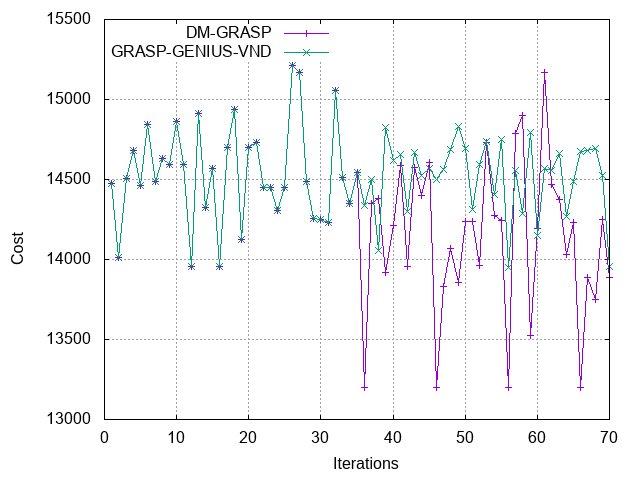
\includegraphics[width=0.8\textwidth]{construcao_grasp_dm-grasp.png}%
\caption{Construction phase}
\label{fig:cdm}
\end{figure}


\begin{figure}[!h]
	\centering

	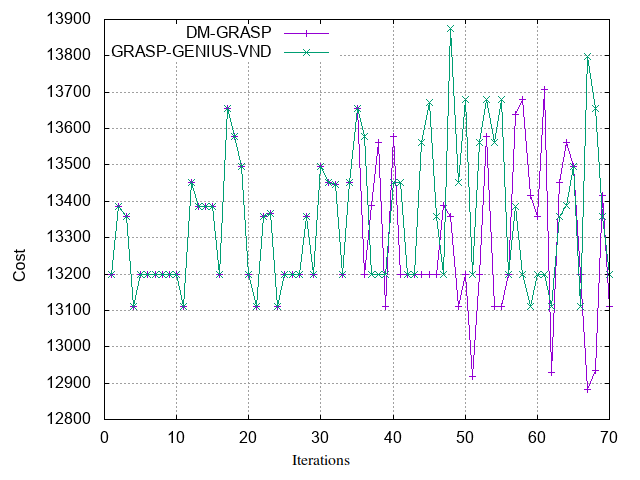
\includegraphics[width=0.8\textwidth]{buscalocal_grasp_dm-grasp.png}%
	\caption{Local search phase}
	\label{fig:bldm}
\end{figure}

\DIFdelbegin \DIFdel{The same analysis with DM-GRASP on the }\DIFdelend %DIF >  The same analysis with DM-GRASP on the impact of using mined patterns was also carried out with MDM-GRASP. From Figures \ref{fig:cmdm} and \ref{fig:blmdm}, it can be observed that after the MD process, the construction and local search phases present similar lines for the two data mining strategies, demonstrating, in this way, similar behaviours. For the instance used in the experiment, MDM-GRASP performed the data mining procedure four times, after iterations 10, 34, 48, and 62. Unlike DM-GRASP, it is possible to verify that MDM-GRASP, after the first run of mining, continues to slightly and gradually reduce the cost of solutions obtained by construction, as patterns are extracted more than once.
\DIFaddbegin 

%DIF >  It is also observed that the proposed strategies are able to better explore the search space. There are several situations where state-of-the-art heuristics perform this exploration inefficiently. For example, in Figure \ref{fig:blmdm}, it can be seen that the value obtained by the GRASP-GENIUS-RVND local search does not change from iterations 5 to 10, 13 to 15, 25 to 27 and 37 to 39 In the specific execution of this experiment, this behaviour tends to occur less when there is an application of MD.

\DIFadd{The }\DIFaddend impact of using mined patterns \DIFdelbegin \DIFdel{was also carried out }\DIFdelend with MDM-GRASP \DIFdelbegin \DIFdel{. From }\DIFdelend \DIFaddbegin \DIFadd{was also analysed, and }\DIFaddend Figures \ref{fig:cmdm} and \ref{fig:blmdm} \DIFdelbegin \DIFdel{, it can be observed that after the MD process, the }\DIFdelend \DIFaddbegin \DIFadd{show similar trends for the }\DIFaddend construction and local search phases \DIFdelbegin \DIFdel{present similar lines for the two }\DIFdelend \DIFaddbegin \DIFadd{of both }\DIFaddend data mining strategies\DIFdelbegin \DIFdel{, demonstrating, in this way, similar behaviours. For the instance used in the experiment, }\DIFdelend \DIFaddbegin \DIFadd{. }\DIFaddend MDM-GRASP performed the data mining procedure four times \DIFaddbegin \DIFadd{during the experiment}\DIFaddend , after iterations 10, 34, 48, and 62. Unlike DM-GRASP, \DIFdelbegin \DIFdel{it is possible to verify that }\DIFdelend MDM-GRASP \DIFdelbegin \DIFdel{, after the first run of mining, continues to slightly and gradually reduce }\DIFdelend \DIFaddbegin \DIFadd{gradually reduces }\DIFaddend the cost of solutions obtained by construction \DIFdelbegin \DIFdel{, }\DIFdelend as patterns are extracted more than once.

\DIFdelbegin \DIFdel{It is also observed that the proposed strategies are able to better explore }\DIFdelend \DIFaddbegin \DIFadd{The proposed strategies also demonstrate a better exploration of }\DIFaddend the search space\DIFdelbegin \DIFdel{. There are several situations where }\DIFdelend \DIFaddbegin \DIFadd{, which is often inefficient with }\DIFaddend state-of-the-art heuristics\DIFdelbegin \DIFdel{perform this exploration inefficiently. For example}\DIFdelend \DIFaddbegin \DIFadd{. For instance}\DIFaddend , in Figure \ref{fig:blmdm}, \DIFdelbegin \DIFdel{it can be seen that }\DIFdelend the value obtained by the GRASP-GENIUS-RVND local search \DIFdelbegin \DIFdel{does not change from iterations5 to 10, 13 to 15}\DIFdelend \DIFaddbegin \DIFadd{remains unchanged during several iterations}\DIFaddend , \DIFdelbegin \DIFdel{25 to 27 and 37 to 39 In the specific execution of this experiment, this behaviour tends to occur less when there is an application of MD }\DIFdelend \DIFaddbegin \DIFadd{but this behaviour is less likely to occur when MD is applied}\DIFaddend .



\begin{figure}[!h]
	\centering
	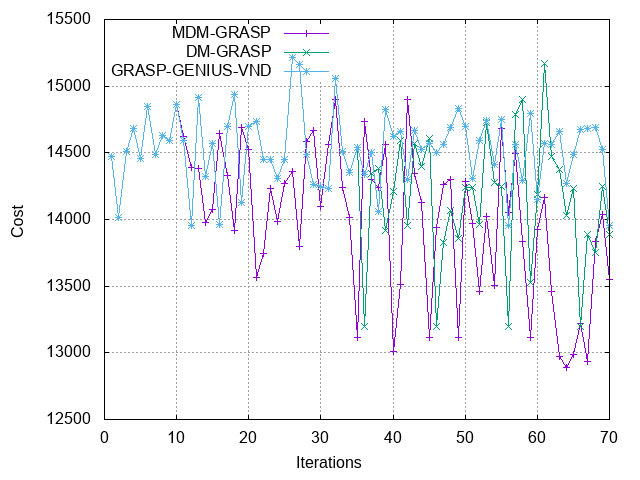
\includegraphics[width=0.7\textwidth]{construcao_mdm_dm_grasp.png}
	\caption{Construction phase}
	\label{fig:cmdm}
\end{figure}


\begin{figure}[!h]
	\centering
	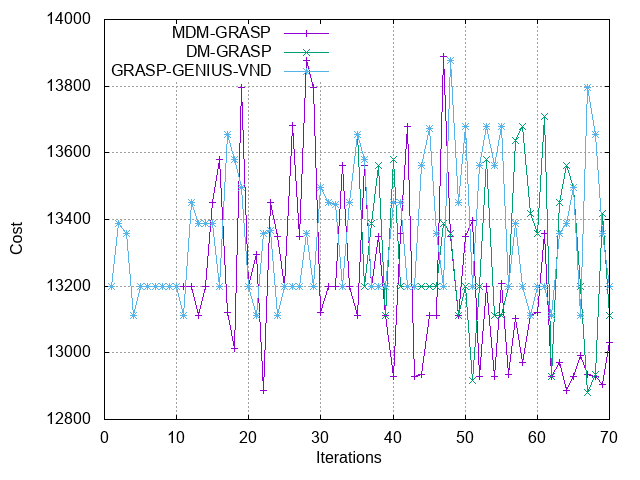
\includegraphics[width=0.7\textwidth]{buscalocal_mdm_dm_grasp.png}
	\caption{Local search phase}
	\label{fig:blmdm}
\end{figure}

\DIFdelbegin \DIFdel{In }\DIFdelend %DIF >  In Tables \ref{tab:dm-grasp} and \ref{tab:mdm-grasp}, it was verified that the main contribution of the MD application in the state-of-the-art heuristic is in the reduction of computational time spent. Figures \ref{fig:md-tempo-c} and \ref{fig:md-tempo-bl} illustrate the behaviour of the construction and local search phases, in terms of computational time used by GRASP-GENIUS-RVND, DM -GRASP and MDM-GRASP, by running 70 iterations of instance g\_kroA150\_VT30\_T30\_W90\_50. The figures show that, for all strategies, the local search phase took more time than the construction phase. Since in the DM-GRASP strategy, the data mining process is executed after iteration 35, it can be seen in Figure \ref{fig:md-tempo-c} that, from this point onwards, the computational time spent by the construction phase is reduced. Originally, the construction of a route is started by selecting three random vertices and then vertices are inserted into the route until all the constraints of the problem are satisfied. With the application of MD, this insertion of vertices takes place from a mined pattern, which usually has more than three vertices, which reduces the number of insertions necessary to satisfy all the conditions of the problem and, consequently, reduces the computational time spent.
\DIFaddbegin 

\DIFaddend Tables \ref{tab:dm-grasp} and \ref{tab:mdm-grasp} \DIFdelbegin \DIFdel{, it was verified }\DIFdelend \DIFaddbegin \DIFadd{demonstrated }\DIFaddend that the main \DIFdelbegin \DIFdel{contribution of the MD application }\DIFdelend \DIFaddbegin \DIFadd{benefit of applying MD }\DIFaddend in the state-of-the-art heuristic is \DIFdelbegin \DIFdel{in the reduction of computational timespent. }\DIFdelend \DIFaddbegin \DIFadd{the reduction in computational time. To illustrate this, }\DIFaddend Figures \ref{fig:md-tempo-c} and \ref{fig:md-tempo-bl} \DIFdelbegin \DIFdel{illustrate }\DIFdelend \DIFaddbegin \DIFadd{show }\DIFaddend the behaviour of the construction and local search phases \DIFdelbegin \DIFdel{, }\DIFdelend in terms of computational time \DIFdelbegin \DIFdel{used by }\DIFdelend \DIFaddbegin \DIFadd{for }\DIFaddend GRASP-GENIUS-RVND, \DIFdelbegin \DIFdel{DM -GRASP }\DIFdelend \DIFaddbegin \DIFadd{DM-GRASP, }\DIFaddend and MDM-GRASP, \DIFdelbegin \DIFdel{by running 70 iterations of }\DIFdelend \DIFaddbegin \DIFadd{using }\DIFaddend instance g\_kroA150\_VT30\_T30\_W90\_\DIFdelbegin \DIFdel{50. The figures show }\DIFdelend \DIFaddbegin \DIFadd{50 with 70 iterations. The figures reveal }\DIFaddend that, for all strategies, the local search phase \DIFdelbegin \DIFdel{took }\DIFdelend \DIFaddbegin \DIFadd{takes }\DIFaddend more time than the construction phase. \DIFdelbegin \DIFdel{Since in }\DIFdelend \DIFaddbegin \DIFadd{In }\DIFaddend the DM-GRASP strategy, the \DIFdelbegin \DIFdel{data mining }\DIFdelend \DIFaddbegin \DIFadd{MD }\DIFaddend process is executed after iteration 35, \DIFdelbegin \DIFdel{it can be seen in Figure \ref{fig:md-tempo-c} }\DIFdelend \DIFaddbegin \DIFadd{and Figure \ref{fig:md-tempo-c} demonstrates }\DIFaddend that, from this point \DIFdelbegin \DIFdel{onwards}\DIFdelend \DIFaddbegin \DIFadd{on}\DIFaddend , the computational time spent \DIFdelbegin \DIFdel{by }\DIFdelend \DIFaddbegin \DIFadd{on }\DIFaddend the construction phase is reduced. Originally, the construction of a route \DIFdelbegin \DIFdel{is started by selecting three random verticesand then }\DIFdelend \DIFaddbegin \DIFadd{begins by randomly selecting three }\DIFaddend vertices\DIFaddbegin \DIFadd{, after which vertices }\DIFaddend are inserted into the route until all \DIFdelbegin \DIFdel{the constraints of the problem }\DIFdelend \DIFaddbegin \DIFadd{problem constraints }\DIFaddend are satisfied. With the application of MD, \DIFdelbegin \DIFdel{this insertion of vertices takes place from a mined pattern, which usually has }\DIFdelend \DIFaddbegin \DIFadd{vertices are inserted using mined patterns, which typically contain }\DIFaddend more than three vertices, \DIFdelbegin \DIFdel{which reduces }\DIFdelend \DIFaddbegin \DIFadd{reducing }\DIFaddend the number of insertions \DIFdelbegin \DIFdel{necessary }\DIFdelend \DIFaddbegin \DIFadd{needed }\DIFaddend to satisfy all the \DIFdelbegin \DIFdel{conditions of the problem }\DIFdelend \DIFaddbegin \DIFadd{constraints }\DIFaddend and, consequently, \DIFdelbegin \DIFdel{reduces }\DIFdelend \DIFaddbegin \DIFadd{reducing }\DIFaddend the computational time spent.

\DIFdelbegin \DIFdel{The }\DIFdelend %DIF >  The GRASP-GENIUS-RVND local search is performed by the RVND heuristic. This strategy is terminated only when all types of Neighbourhoods are explored, and for each new solution improvement, RVND restarts its process from the first Neighbourhood in the list. As the solutions generated by the construction from the patterns are generally closer to an optimal location, in Figure \ref{fig:md-tempo-bl}, it can be observed that the exploration of all types of Neighbourhoods is performed more quickly, as fewer improvements are made, and RVND returns fewer times to the first Neighbourhood in the list.
\DIFaddbegin 

%DIF >  In the MDM-GRASP strategy, the data mining process is performed more than once. As can be seen in Figures \ref{fig:md-tempo-c} and \ref{fig:md-tempo-bl}, MDM-GRASP behaves similarly to DM-GRASP until the moment when the first mining is carried out. From this iteration onwards, the more MD processes are executed, the computational times of the construction and local search phases are gradually and slightly reduced.

\DIFadd{The RVND heuristic is used for the }\DIFaddend GRASP-GENIUS-RVND \DIFdelbegin \DIFdel{local search is performed by the RVND heuristic . This strategy is terminated only when }\DIFdelend \DIFaddbegin \DIFadd{local search, which explores }\DIFaddend all types of \DIFdelbegin \DIFdel{Neighbourhoods are explored, and for each new solution improvement }\DIFdelend \DIFaddbegin \DIFadd{neighbourhoods until there are no more improvements. Each time a new improvement is made}\DIFaddend , RVND restarts its process from the first \DIFdelbegin \DIFdel{Neighbourhood }\DIFdelend \DIFaddbegin \DIFadd{neighbourhood }\DIFaddend in the list. \DIFdelbegin \DIFdel{As }\DIFdelend \DIFaddbegin \DIFadd{Since }\DIFaddend the solutions generated \DIFdelbegin \DIFdel{by the construction from the patterns are generally }\DIFdelend \DIFaddbegin \DIFadd{from pattern construction are typically }\DIFaddend closer to an optimal \DIFdelbegin \DIFdel{location, }\DIFdelend \DIFaddbegin \DIFadd{solution, as seen }\DIFaddend in Figure \ref{fig:md-tempo-bl}, \DIFdelbegin \DIFdel{it can be observed that }\DIFdelend the exploration of all \DIFdelbegin \DIFdel{types of Neighbourhoods is performed more quickly, }\DIFdelend \DIFaddbegin \DIFadd{neighbourhoods is completed faster }\DIFaddend as fewer improvements are made, and RVND returns fewer times to the first \DIFdelbegin \DIFdel{Neighbourhood }\DIFdelend \DIFaddbegin \DIFadd{neighbourhood }\DIFaddend in the list.

In the MDM-GRASP strategy, the data mining process is performed \DIFdelbegin \DIFdel{more than once. As can be seen }\DIFdelend \DIFaddbegin \DIFadd{multiple times. As shown }\DIFaddend in Figures \ref{fig:md-tempo-c} and \ref{fig:md-tempo-bl}, MDM-GRASP behaves similarly to DM-GRASP until the \DIFdelbegin \DIFdel{moment when the first mining is carried out}\DIFdelend \DIFaddbegin \DIFadd{first mining process is performed}\DIFaddend . From this \DIFdelbegin \DIFdel{iteration onwards, the more MD }\DIFdelend \DIFaddbegin \DIFadd{point on, as more mining }\DIFaddend processes are executed, the computational times \DIFdelbegin \DIFdel{of }\DIFdelend \DIFaddbegin \DIFadd{for }\DIFaddend the construction and local search phases are gradually and slightly reduced.

\begin{figure}[!h]
	\centering
	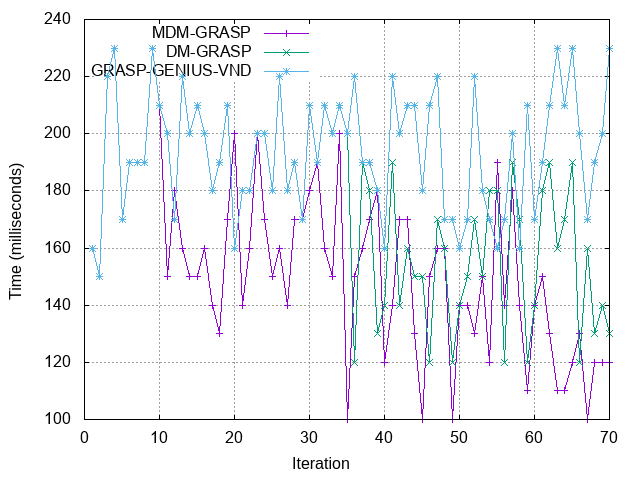
\includegraphics[width=0.7\textwidth]{md-tempo-construcao.png}
	\caption{Construction phase}
	\label{fig:md-tempo-c}
\end{figure}

\begin{figure}[!h]
	\centering
	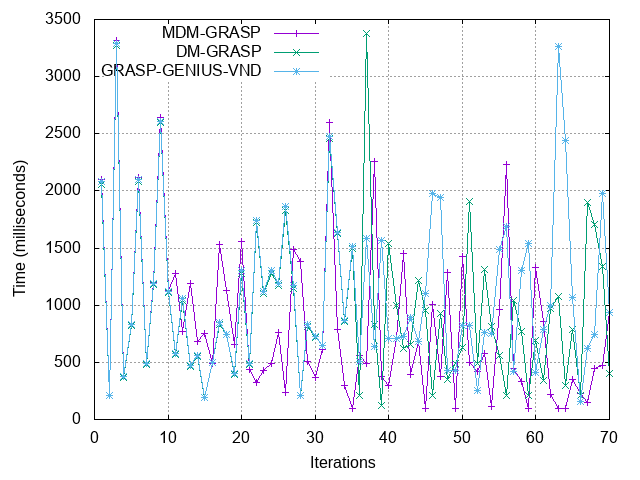
\includegraphics[width=0.7\textwidth]{md-tempo-bl.png}
	\caption{Local search phase}
	\label{fig:md-tempo-bl}
\end{figure}

\subsection{Statistical tests}

\DIFdelbegin \DIFdel{To strengthen the performance evaluation }\DIFdelend %DIF >  To strengthen the performance evaluation of the proposed methods, statistical significance tests (SST) were performed in all instances. Through the application of this test, the objective is to verify, in statistical terms, whether the results generated by the heuristics indicate a statistical difference, reinforcing the relevance of the application of MD, or not.
\DIFaddbegin 


%DIF >  Generally, this type of test is used to evaluate algorithms that have random components, and identify whether
%DIF >  the difference between their means was due to the superiority of one of these algorithms or just due to the randomness present in the methods. In this work, the non-parametric statistical test of \textit{Friedman} \cite{siegal1956nonparametric} of the R package \cite{r-package} was used, which does not require that the analysed sample follow a normal distribution.

%DIF >  To perform this test, the costs obtained for ten executions of each heuristic were considered, $p$-value equal to 0.05 and two hypotheses:

%DIF >  \begin{itemize}
%DIF >  \item Null Hypothesis ($H_0$): There is no difference between the means found by the two methods; and

%DIF >  \item Alternative hypothesis ($H_1$): There is a difference between the means found by the two methods.
%DIF >  \end{itemize}

\DIFadd{In order to enhance the assessment }\DIFaddend of the proposed methods, statistical significance tests (\DIFdelbegin \DIFdel{SST) were performed in }\DIFdelend \DIFaddbegin \DIFadd{SSTs) were conducted for }\DIFaddend all instances. \DIFdelbegin \DIFdel{Through the application }\DIFdelend \DIFaddbegin \DIFadd{The purpose }\DIFaddend of this test \DIFdelbegin \DIFdel{, the objective is to verify}\DIFdelend \DIFaddbegin \DIFadd{is to determine}\DIFaddend , in statistical terms, whether the results \DIFdelbegin \DIFdel{generated }\DIFdelend \DIFaddbegin \DIFadd{obtained }\DIFaddend by the heuristics \DIFdelbegin \DIFdel{indicate }\DIFdelend \DIFaddbegin \DIFadd{show }\DIFaddend a statistical difference, \DIFdelbegin \DIFdel{reinforcing the relevance of the application of MDand PLI}\DIFdelend \DIFaddbegin \DIFadd{thus reinforcing the significance of applying MD}\DIFaddend , or not.

\DIFdelbegin \DIFdel{Generally}\DIFdelend \DIFaddbegin \DIFadd{Typically}\DIFaddend , this type of test is used to evaluate algorithms that \DIFdelbegin \DIFdel{have random components , and identify }\DIFdelend \DIFaddbegin \DIFadd{involve random components and to determine }\DIFaddend whether the difference between their means \DIFdelbegin \DIFdel{was }\DIFdelend \DIFaddbegin \DIFadd{is }\DIFaddend due to the superiority of one of \DIFdelbegin \DIFdel{these algorithms or just due }\DIFdelend \DIFaddbegin \DIFadd{the algorithms or simply }\DIFaddend to the randomness present in the methods. In this \DIFdelbegin \DIFdel{work}\DIFdelend \DIFaddbegin \DIFadd{study}\DIFaddend , the non-parametric statistical test of \DIFdelbegin \textit{\DIFdel{Friedman}} %DIFAUXCMD
\DIFdel{\mbox{%DIFAUXCMD
\cite{siegal1956nonparametric}}\hskip0pt%DIFAUXCMD
of }\DIFdelend \DIFaddbegin \DIFadd{Friedman \mbox{%DIFAUXCMD
\cite{siegal1956nonparametric}}\hskip0pt%DIFAUXCMD
, available in }\DIFaddend the R package \cite{r-package}\DIFdelbegin \DIFdel{was used, which }\DIFdelend \DIFaddbegin \DIFadd{, was used. This test }\DIFaddend does not require \DIFdelbegin \DIFdel{that the analysed sample }\DIFdelend \DIFaddbegin \DIFadd{the analyzed sample to }\DIFaddend follow a normal distribution.

To perform \DIFdelbegin \DIFdel{this }\DIFdelend \DIFaddbegin \DIFadd{the }\DIFaddend test, the costs obtained \DIFdelbegin \DIFdel{for ten executions }\DIFdelend \DIFaddbegin \DIFadd{from ten runs }\DIFaddend of each heuristic were considered, \DIFaddbegin \DIFadd{with a }\DIFaddend $p$-value \DIFdelbegin \DIFdel{equal to }\DIFdelend \DIFaddbegin \DIFadd{of }\DIFaddend 0.05 and two hypotheses:

\begin{itemize}
\item Null \DIFdelbegin \DIFdel{Hypothesis }\DIFdelend \DIFaddbegin \DIFadd{hypothesis }\DIFaddend ($H_0$): There is no difference between the means \DIFdelbegin \DIFdel{found }\DIFdelend \DIFaddbegin \DIFadd{obtained }\DIFaddend by the two methods; and
\DIFdelbegin %DIFDELCMD < 

%DIFDELCMD < %%%
\DIFdelend \item Alternative hypothesis ($H_1$): There is a difference between the means \DIFdelbegin \DIFdel{found }\DIFdelend \DIFaddbegin \DIFadd{obtained }\DIFaddend by the two methods.
\end{itemize}


In this sense, $H_0$ will be rejected with 95\% certainty if, for each instance, the test of \textit{Friedman} \cite{siegal1956nonparametric} returns a value less than the defined $p$-value.
If $H_0$ is rejected, the alternative hypothesis $H_1$ is considered.

In Table \ref{tab:sig1}, for each pair of compared heuristics, the number of wins, losses and ties in terms of \DIFaddbegin \DIFadd{the }\DIFaddend best solution, average solution and average time spent is shown. For the solution mean, the values in parentheses indicate the number of statistically significant results. MDM-GRASP was not directly compared with the state-of-the-art heuristic, but with DM-GRASP in Table \ref{tab:mdm-grasp}. Table \ref{tab:sig1}, presents a summary of what can be deduced from Tables \ref{tab:dm-grasp} and \ref{tab:mdm-grasp}, \DIFdelbegin \DIFdel{in relation to }\DIFdelend \DIFaddbegin \DIFadd{about }\DIFaddend a comparison between MDM- GRASP and GRASP-GENIUS-RVND.

\begin{table}[!h]
\centering
\caption{Summary of results and statistical significance test between GRASP-GENIUS-RVND and MDM-GRASP.}
\label{tab:sig1}
\begin{tabular}{llll}
\hline
& Best Sol. & Average Sol. & Average T(s) \\
\hline
\begin{tabular}[c]{@{}l@{}}Win\\ MDM-GRASP\end{tabular} & 13 & 41 (10)& 105 \\ \hline
Ties & 90 & 50 & 0 \\ \hline
\begin{tabular}[c]{@{}l@{}}Win\\ GRASP-GENIUS-RVND\end{tabular} & 4 & 16 (0) & 2\\
\hline
\end{tabular}
\end{table}

In terms of the best solution, MDM-GRASP was superior in 13, tied in 90 and lost in 4 instances. Regarding the average solution, the mining heuristic won in 41 cases, ten of which were statistically significant, tied in 50 and lost in 16 instances. For this statistical test, it was observed that the significant results obtained are concentrated in the larger instances, including gr202\_R39\_T122\_W41\_25, gr229\_R45\_T46\_W138\_25, lin318\_R108\_T105\_W105 \_50, rd400\_R80\_T240\_W80\_25, among others. As already noted in previous sections, the application of data mining reduces the computational time of the heuristics. With MDM-GRASP it was no different, being faster than the state-of-the-art heuristic in 105 of the 107 instances tested, and with an average CPU-time reduction of 23.55\% per instance.

\subsection{TTTPlots}

A final comparison was made between the proposed methods and the state-of-the-art, using \textit{Time-to-target plots} (\texttt{TTTplots}) \cite{aiex2007ttt}. These types of plots are used to analyse the behaviour of algorithms with random components and show the cumulative probability of an algorithm to find a solution better than or equal to a predefined target solution value, in a certain running time.

The TTTplots illustrated in Figure \ref{fig:tttplots1} were generated from 100 executions of the GRASP-GENIUS-RVND and MDM-GRASP methods using the instance g\_kroA150\_VT30\_T30\_W90\_50, and  seeds ranging from 1 to 100. For the behaviour analysis, a difficult target value was chosen, the value of the best solution reported in this instance by GRASP-GENIUS-RVND (12918).

\begin{figure}[!h]
\centering
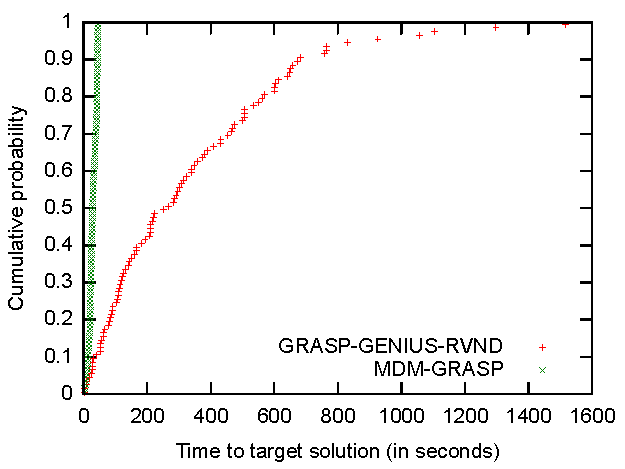
\includegraphics[width=0.7\textwidth]{tttplot.pdf}
\caption{TTTplots for instance g\_kroA150\_VT30\_T30\_W90\_50, target: 12962.}
\label{fig:tttplots1}%
\end{figure}

From Figure \ref{fig:tttplots1}, a large difference can be seen between the curves of the compared heuristics. After 561 seconds of execution, GRASP-GENIUS-RVND reaches the target with a probability of 79\%, while with that same chance, MDM-GRASP only needs 41.71 seconds to reach the target.

\section{Conclusions}

\label{sec:conclusions}

In \DIFdelbegin \DIFdel{this work, we have }\DIFdelend \DIFaddbegin \DIFadd{conclusion, this study }\DIFaddend proposed two hybrid heuristics, DM-GRASP and MDM-GRASP, \DIFdelbegin \DIFdel{using DM }\DIFdelend \DIFaddbegin \DIFadd{which utilize data mining }\DIFaddend techniques over a state-of-the-art heuristic\DIFdelbegin \DIFdel{(}\DIFdelend \DIFaddbegin \DIFadd{, }\DIFaddend GRASP-GENIUS-RVND\DIFdelbegin \DIFdel{). These heuristics perform data mining along the iterative process of the GRASP-GENIUS-RVND and extract patterns detected in high- quality solutions, which are used to generate further initial solutions. 
}%DIFDELCMD < 

%DIFDELCMD < %%%
\DIFdel{As the source-code was provided by the authors, all GRASP-GENIUS-RVND experiments mentioned in \mbox{%DIFAUXCMD
\citet{daSilva} }\hskip0pt%DIFAUXCMD
were completely re-executed in order to offer a fair and strict evaluation of the computational results. In addition, to assist the evaluation of the heuristics,  examples of the influence of mining patterns on early solutions, analyses of time convergence (TTTplots), and }\DIFdelend \DIFaddbegin \DIFadd{. The heuristics were evaluated using various methods, including the re-execution of all experiments and the use of }\DIFaddend statistical significance tests\DIFdelbegin \DIFdel{were performed. }%DIFDELCMD < 

%DIFDELCMD < %%%
\DIFdel{The reported results demonstrated }\DIFdelend \DIFaddbegin \DIFadd{. The results showed }\DIFaddend that both DM strategies \DIFdelbegin \DIFdel{perform better than }\DIFdelend \DIFaddbegin \DIFadd{outperformed }\DIFaddend the state-of-the-art heuristic \DIFdelbegin \DIFdel{, }\DIFdelend in terms of solution quality and CPU time\DIFdelbegin \DIFdel{simultaneously.
Both DM-GRASP and MDM-GRASP heuristics managed to apply a significant reduction in }\DIFdelend \DIFaddbegin \DIFadd{.
}

\DIFadd{Furthermore, the heuristics were able to significantly reduce the }\DIFaddend execution time, \DIFdelbegin \DIFdel{confirming the various reports in the literature on the application of such }\DIFdelend \DIFaddbegin \DIFadd{which confirms the effectiveness of using data mining }\DIFaddend techniques. MDM-GRASP \DIFdelbegin \DIFdel{, for example, which was the heuristic with the best performance }\DIFdelend \DIFaddbegin \DIFadd{was found to be the best-performing heuristic }\DIFaddend among the three compared, \DIFdelbegin \DIFdel{was able to reduce the GRASP-GENIUS-RVND time by }\DIFdelend \DIFaddbegin \DIFadd{achieving an }\DIFaddend 88.1\% \DIFdelbegin \DIFdel{for the instancepr226\_R44\_T46\_W136\_75.
}\DIFdelend \DIFaddbegin \DIFadd{reduction in execution time for a specific instance.
}\DIFaddend 

\DIFdelbegin \DIFdel{As a further investigation, we intend to combine the }\DIFdelend \DIFaddbegin \DIFadd{Future work will focus on combining }\DIFaddend MDM-GRASP with integer programming techniques \DIFdelbegin \DIFdel{. Since it was observed that mined patterns can help in the construction of initial solutions, we see the possibility of applying them to }\DIFdelend \DIFaddbegin \DIFadd{to explore the possibility of using mined patterns to assist in }\DIFaddend the exact resolution of \DIFdelbegin \DIFdel{an IP model through branch-and-bound, on fixing variables, providing a ``warm start'', or guiding the }\DIFdelend \DIFaddbegin \DIFadd{integer programming models through warm starts or guiding }\DIFaddend variable selection for branching\DIFaddbegin \DIFadd{. Overall, this study has demonstrated the potential of using data mining techniques to enhance the performance of existing heuristics}\DIFaddend .







%\bibliographystyle{model1-num-names}
\bibliographystyle{apalike}

% Loading bibliography database
\bibliography{cas-refs}


\end{document}

